\chapter{AHTR Plank Optimization Results}
\glsresetall
\label{chap:ahtr-plank-opt-results}
In this chapter, I report the \gls{AHTR} plank's \gls{ROLLO} optimization results. 
I vary the following \gls{AHTR} plank input parameters:
\begin{itemize}
    \item \gls{TRISO} packing fraction distribution ($\rho_{TRISO}(\vec{r})$),
    \item total fuel packing fraction ($PF_{total}$), and 
    \item coolant channel shape
\end{itemize} 
Section \ref{sec:input-parameter-modeling} detailed how I vary these 
\gls{AHTR} one-third assembly's input parameters. 
I optimize the \gls{AHTR} plank for the following objectives:
\begin{itemize}
    \item minimize total fuel packing fraction ($PF_{total}$), 
    \item minimize maximum plank temperature ($T_{max}$), and
    \item minimize fuel-normalized power peaking factor ($PPF_{fuel}$)
\end{itemize} 
Table \ref{tab:objectives-2} outlines these objectives and their motivation.
\begin{table}[htbp]
    \centering
    \onehalfspacing
    \caption{\acrfull{ROLLO} \acrfull{AHTR} optimization problem objectives with 
    their quantification descriptions and motivation.}
	\label{tab:objectives-2}
    \footnotesize
    \begin{tabular}{p{4.5cm}|p{5cm}p{5cm}}
    \hline 
    \textbf{Objective}& \textbf{Quantification}& \textbf{Motivation} \\
    \hline
    \textbf{Minimize fuel amount} & Minimize total fuel packing \newline fraction 
    & Cost savings, Non-proliferation \\ 
    \hline
    \textbf{Maximize heat transfer} & Minimize maximum temperature 
    & Minimize thermal stress in the fuel \\
    \hline
    \textbf{Minimize power peaking} & Minimize power peaking factor normalized by fuel distribution 
    & Efficient fuel utilization, longer core life, safety\\
    \hline
    \end{tabular}
\end{table}
Chapter \ref{chap:method} detailed the methodology for \gls{AHTR} plank modeling 
and \gls{ROLLO} optimization. 

The subsequent sections outline the \gls{AHTR} plank optimization simulations 
(Section \ref{sec:plank-overview}), describe the single-objective (Section 
\ref{sec:plank-one-obj}), two-objective (Section \ref{sec:plank-two-obj}), and 
three-objective (Section \ref{sec:plank-three-obj}) \gls{ROLLO} optimization 
simulation results, and report each simulation's computational cost 
(Section \ref{sec:plank-compute-cost}).
The \texttt{plank-optimization} directory in the \\ \texttt{arfc/2022-chee-dissertation} 
Github repository contains the data and analysis associated with this 
chapter's results \cite{chee_dissertation_2021}. 
% TODO: add reference to reproducibility appendix. 

\section{ROLLO AHTR Plank Optimization Simulations Overview}
\label{sec:plank-overview}
In this chapter, I conducted single objective, single input parameter 
\gls{ROLLO} optimizations to understand the individual impacts of each objective on 
each input parameter for the \gls{AHTR} plank model. 
Their results are then used to inform the multi-objective optimization simulations setup. 
Table \ref{tab:slab-obj-breakdown} summarizes the details of each \gls{ROLLO} 
optimization simulation conducted in this chapter.
\begin{table}[htbp!]
    \centering
    \onehalfspacing
    \caption{\gls{ROLLO} simulations for optimizing \gls{AHTR} plank. 
    There are six single objective optimization simulations (p-1a to p-1f) that are 
    used to understand the individual impacts of each objective on each input parameter. 
    Their results are then used to inform the multi-objective optimization simulations 
    (p-2a, p-2b, p-2c, p-3a, p-3b) setup.
    $PF_{total}$: Total fuel packing fraction; 
    $T_{max}$: Maximum plank temperature;
    $PPF_{fuel}$: Fuel-normalized power peaking factor; 
    $\rho_{TRISO}(\vec{r})$: \gls{TRISO} particle distribution.}
	\label{tab:slab-obj-breakdown}
    \footnotesize
    \begin{tabular}{p{1.5cm}|l|llll}
    \hline 
    \textbf{Objs [\#]} & \textbf{Sim} & \textbf{Objectives} & \textbf{Constraints} &\textbf{Varying Parameters} & \textbf{Simulation Software} \\
    \hline
    \multirow{7}{2cm}{1} & p-1a & \tabitem min($PF_{total}$) & \tabitem $k_{eff}$ $\geq$ 1.35 &\tabitem $\rho_{TRISO}(\vec{r})$ & OpenMC \\
    & & & & \tabitem $PF_{total}$ & \\
    \cline{2-6}
    & p-1b & \tabitem min($T_{max}$) & \tabitem $k_{eff}$ $\geq$ 1.00 &\tabitem $\rho_{TRISO}(\vec{r})$ & OpenMC, Moltres\\
    \cline{2-6}
    & p-1c & \tabitem min($PPF_{fuel}$) & \tabitem $k_{eff}$ $\geq$ 1.00 &\tabitem $\rho_{TRISO}(\vec{r})$ & OpenMC\\
    \cline{2-6}
    & p-1d & \tabitem min($PF_{total}$) & \tabitem $k_{eff}$ $\geq$ 1.35 &\tabitem Coolant channel shape & OpenMC \\
    & & & & \tabitem $PF_{total}$ & \\
    \cline{2-6}
    & p-1e & \tabitem min($T_{max}$) & \tabitem $k_{eff}$ $\geq$ 1.35 &\tabitem Coolant channel shape & OpenMC, Moltres\\
    \cline{2-6}
    & p-1f & \tabitem min($PPF_{fuel}$) & \tabitem $k_{eff}$ $\geq$ 1.35 &\tabitem Coolant channel shape & OpenMC\\
    \hline
    \multirow{6}{2cm}{2}& p-2a & \tabitem min($PF_{total}$) & \tabitem $k_{eff}$ $\geq$ 1.35 & \tabitem $\rho_{TRISO}(\vec{r})$ & OpenMC, Moltres\\
    & &\tabitem min($T_{max}$) & & \tabitem $PF_{total}$ & \\
    \cline{2-6}
    & p-2b & \tabitem min($PF_{total}$) & \tabitem $k_{eff}$ $\geq$ 1.35 & \tabitem $\rho_{TRISO}(\vec{r})$ & OpenMC\\
    & & \tabitem min($PPF_{fuel}$) & & \tabitem $PF_{total}$ & \\
    \cline{2-6}
    & p-2c & \tabitem min($T_{max}$) & \tabitem $k_{eff}$ $\geq$ 1.00 & \tabitem $\rho_{TRISO}(\vec{r})$ & OpenMC, Moltres\\
    & & \tabitem min($PPF_{fuel}$) & & & \\
    \hline
    \multirow{6}{2cm}{3}& p-3a &\tabitem min($PF_{total}$) & \tabitem $k_{eff}$ $\geq$ 1.35 & \tabitem $\rho_{TRISO}(\vec{r})$ & OpenMC, Moltres\\
    && \tabitem min($PPF_{fuel}$) & & \tabitem $PF_{total}$ & \\
    && \tabitem min($T_{max}$) & & & \\
    \cline{2-6}
    & p-3b &\tabitem min($PF_{total}$) & \tabitem $k_{eff}$ $\geq$ 1.35 & \tabitem $\rho_{TRISO}(\vec{r})$ & OpenMC, Moltres\\
    && \tabitem min($PPF_{fuel}$) & & \tabitem $PF_{total}$ & \\
    && \tabitem min($T_{max}$) & & \tabitem Coolant channel shape& \\
    \hline
    \end{tabular}
\end{table}

$k_{eff}$ strongly correlates with total fuel packing fraction ($PF_{total}$). 
The \gls{AHTR} plank with the same $PF_{total}$ as the \gls{FHR} benchmark's 
assembly model had a $k_{eff}$ of 1.35. 
For optimization simulations that vary $PF_{total}$, I constrained $k_{eff} \geq 1.35$ 
to find optimal input parameters that achieve similar performance to the original 
benchmark \gls{TRISO} distribution. 
For the optimization simulations that do not vary $PF_{total}$, I use 
$PF_{total} = 0.0979$, which corresponds to the \gls{FHR} benchmark's $PF_{total}$, 
and constrained $k_{eff} \geq 1.00$. 
Thus, the $k_{eff}$ constraint values used are $1.35$ and $1.00$ for optimization 
simulations that do and do not vary total packing fraction, respectively. 

Simulations are run on the BlueWaters supercomputer \cite{ncsa_about_2017} and Theta 
supercomputer at the Argonne Leadership Computing Facility under the Director's 
Discretionary Allocation Program \cite{noauthor_argonne_2022}. 
Section \ref{sec:plank-compute-cost} details the computational 
cost of each optimization simulation.  

\section{AHTR Plank: Single-Objective Optimization Results}
\label{sec:plank-one-obj}
This section reports the \gls{AHTR} plank's \gls{ROLLO} single-objective 
optimization results. 
Table \ref{tab:slab-obj-breakdown} summarizes the parameters for the single-objective 
simulations that are presented in this section: p-1a, p-1b, p-1c, p-1d, p-1e, and p-1f. 
In the following subsections, I describe the single-objective simulation results 
grouped by the minimized objective (Sections \ref{sec:plank-1-obj-pf}, 
\ref{sec:plank-1-obj-temp}, and \ref{sec:plank-1-obj-ppf}), and provide discussion 
about the single-objective simulations results (Section 
\ref{sec:plank-discussion-single}).

If a single-objective optimization problem's objective converges earlier than the 
five generations I intended to run (determined in Section 
\ref{sec:multi-obj-hyperparameters}), I stop the simulation at that generation to 
save computational resources as the solution will not change.
However, if the problem's objective does not converge by generation 5, I run the 
problem for a few more generations until satisfactory convergence is reached.
Section \ref{sec:rollo-convergence} described how reactor designers can use 
\gls{ROLLO} to determine problem convergence. 

\subsection{Objective: Minimize Total Packing Fraction ($PF_{total}$)}
\label{sec:plank-1-obj-pf}
This section describes the single-objective p-1a and p-1d optimization simulation
results. 
Both simulations minimize the total fuel packing fraction ($PF_{total}$) objective. 
The minimize $PF_{total}$ objective is important because a reactor that uses less fuel
with similar performance enables cost savings. 
Simulation p-1a varies the total fuel packing fraction ($PF_{total}$) and \gls{TRISO} 
packing fraction distribution ($\rho_{TRISO}(\vec{r})$), while simulation p-1d varies 
the total fuel packing fraction ($PF_{total}$) and coolant channel shape. 

\subsubsection{Simulation p-1a: Variation of $\rho_{TRISO}(\vec{r})$ and $PF_{total}$}
Table \ref{tab:simulationp1a} summarizes the optimization problem parameters for 
simulation p-1a. 
\begin{table}[htbp!]
    \centering
    \onehalfspacing
    \caption{Simulation p-1a optimization problem parameters.}
	\label{tab:simulationp1a}
    \footnotesize
    \begin{tabular}{l|p{4cm}}
    \hline 
    \multicolumn{2}{c}{\textbf{Single Objective: Simulation p-1a}} \\
    \hline 
    \textbf{Objectives} & Minimize $PF_{total}$ \\
    \hline 
    \textbf{Input parameter variations} & $0.02 \leq PF_{total} \leq 0.04$ \\
    & $\rho_{TRISO}(\vec{r})$: $0<a<2$ \\
    & $\rho_{TRISO}(\vec{r})$: $0<b<\frac{\pi}{2}$ \\
    & $\rho_{TRISO}(\vec{r})$: $0<c<2\pi$ \\
    \hline
    \textbf{Constraints} & $k_{eff} \geq 1.35$\\ 
    \hline 
    \textbf{Genetic algorithm parameters} & Population size: 64 \\
    & Generations: 10 \\
    \hline
    \end{tabular}
\end{table}
Figure \ref{fig:slab-obj-1-pf-evol} shows the $PF_{total}$ evolution,  
Figure \ref{fig:slab-obj-1-pf-final} shows the five TRISO packing fraction 
distributions ($\rho_{TRISO}(\vec{r})$) in the final generation with the 
most-minimized $PF_{total}$, and Figure \ref{fig:slab-obj-1-pf-most-minimized} 
illustrates the \gls{AHTR} plank model with the most-minimized $PF_{total}$.
\begin{figure}[htbp!]
    \centering
    \begin{subfigure}{0.9\textwidth}
        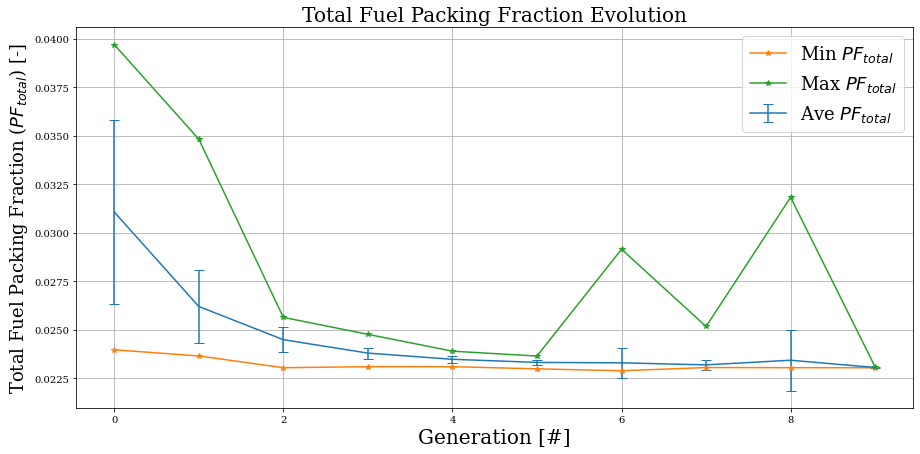
\includegraphics[width=\linewidth]{slab-obj-1-pf-evol.png}
        \caption{Minimum, average, and maximum $PF_{total}$ evolution of the 
        population in each generation.}
        \label{fig:slab-obj-1-pf-evol} 
    \end{subfigure}
    \begin{subfigure}{0.9\textwidth}
        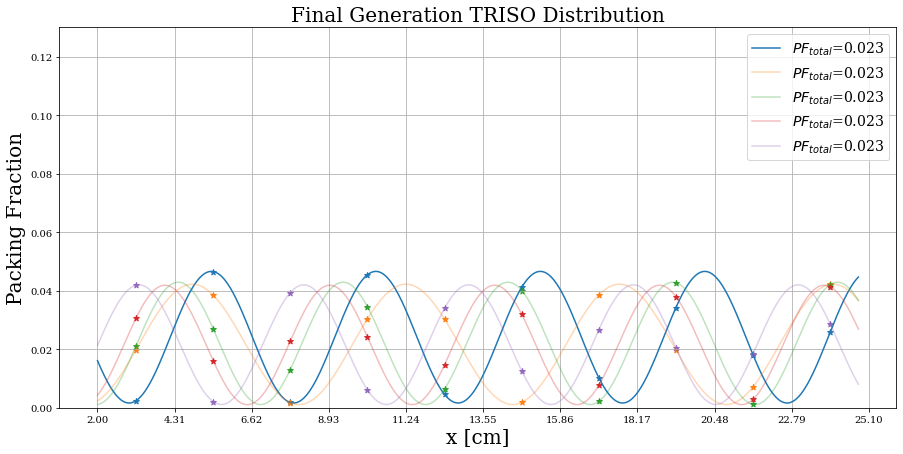
\includegraphics[width=\linewidth]{slab-obj-1-pf-final.png}
        \caption{TRISO packing fraction distribution for the five reactor models with the 
        smallest $PF_{total}$ in the final generation.}
        \label{fig:slab-obj-1-pf-final} 
    \end{subfigure}
    \begin{subfigure}{0.9\textwidth}
        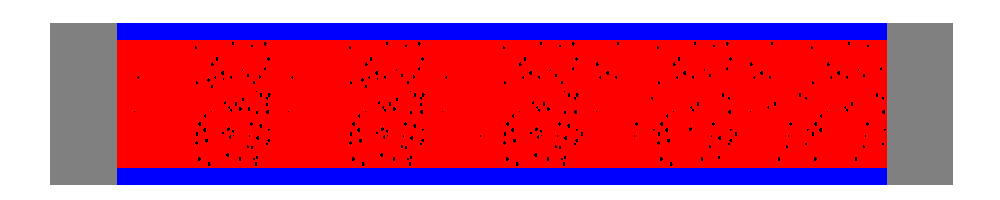
\includegraphics[width=\linewidth]{slab-obj-1-pf-most-minimized.png}
        \caption{\gls{AHTR} plank model with the most-minimized $PF_{total}$ 
        (corresponds to the blue solid distribution in Figure 
        \ref{fig:slab-obj-1-pf-final}).}
        \label{fig:slab-obj-1-pf-most-minimized} 
    \end{subfigure}
    \caption{Simulation p-1a -- ROLLO single-objective optimization to minimize the 
    total fuel packing fraction ($PF_{total}$). 
    Input parameters varied: total fuel packing fraction 
    ($PF_{total}$), \gls{TRISO} packing fraction distribution ($\rho_{TRISO}(\vec{r})$).}
    \label{fig:slab-obj-1-pf}
\end{figure}
Figure \ref{fig:slab-obj-1-pf-evol} shows that the minimum and average $PF_{total}$ 
converged quickly. 
The final generation's average $PF_{total}$ values for all reactor models 
converged to approximately 0.023. 
In Figure \ref{fig:slab-obj-1-pf-final}, the \gls{TRISO} packing fraction
distributions are not the same but follow a similar oscillating 
TRISO distribution pattern. 
Because it is more productive to compare all of the single objective results to one 
another, Section \ref{sec:plank-discussion-single} discusses the driving factors for
the minimize $PF_{total}$ objective and explains simulation p-1a's most-minimized 
$PF_{total}$ oscillating TRISO distribution. 

\subsubsection{Simulation p-1d: Variation of $PF_{total}$ and Coolant channel shape}
Table \ref{tab:simulationp1d} summarizes the optimization problem parameters for 
simulation p-1d.  
\begin{table}[htbp!]
    \centering
    \onehalfspacing
    \caption{Simulation p-1d optimization problem parameters.}
	\label{tab:simulationp1d}
    \footnotesize
    \begin{tabular}{l|p{6.5cm}}
    \hline 
    \multicolumn{2}{c}{\textbf{Single Objective: Simulation p-1d}} \\
    \hline 
    \textbf{Objectives} & Minimize $PF_{total}$\\
    \hline 
    \textbf{Input parameter variations} & $0.02 \leq PF_{total} \leq 0.04$ \\
    & Coolant channel shape: $0.05<r_{top}<0.35$ \\
    & Coolant channel shape: $0.05<r_{bot}<0.35$ \\
    \hline
    \textbf{Constraints} & $k_{eff} \geq 1.35$\\ 
    \hline 
    \textbf{Genetic algorithm parameters} & Population size: 64 \\
    & Generations: 3 \\
    \hline
    \end{tabular}
\end{table}
Figure \ref{fig:slab-obj-1-pf-evol-coolant} shows the $PF_{total}$ evolution converges 
over three generations.  
Figure \ref{fig:slab-obj-1-pf-final-coolant} shows plots of $r_{top}$ and $r_{bot}$ 
against $PF_{total}$.  
\begin{figure}[htbp!]
    \centering
    \begin{subfigure}{\textwidth}
        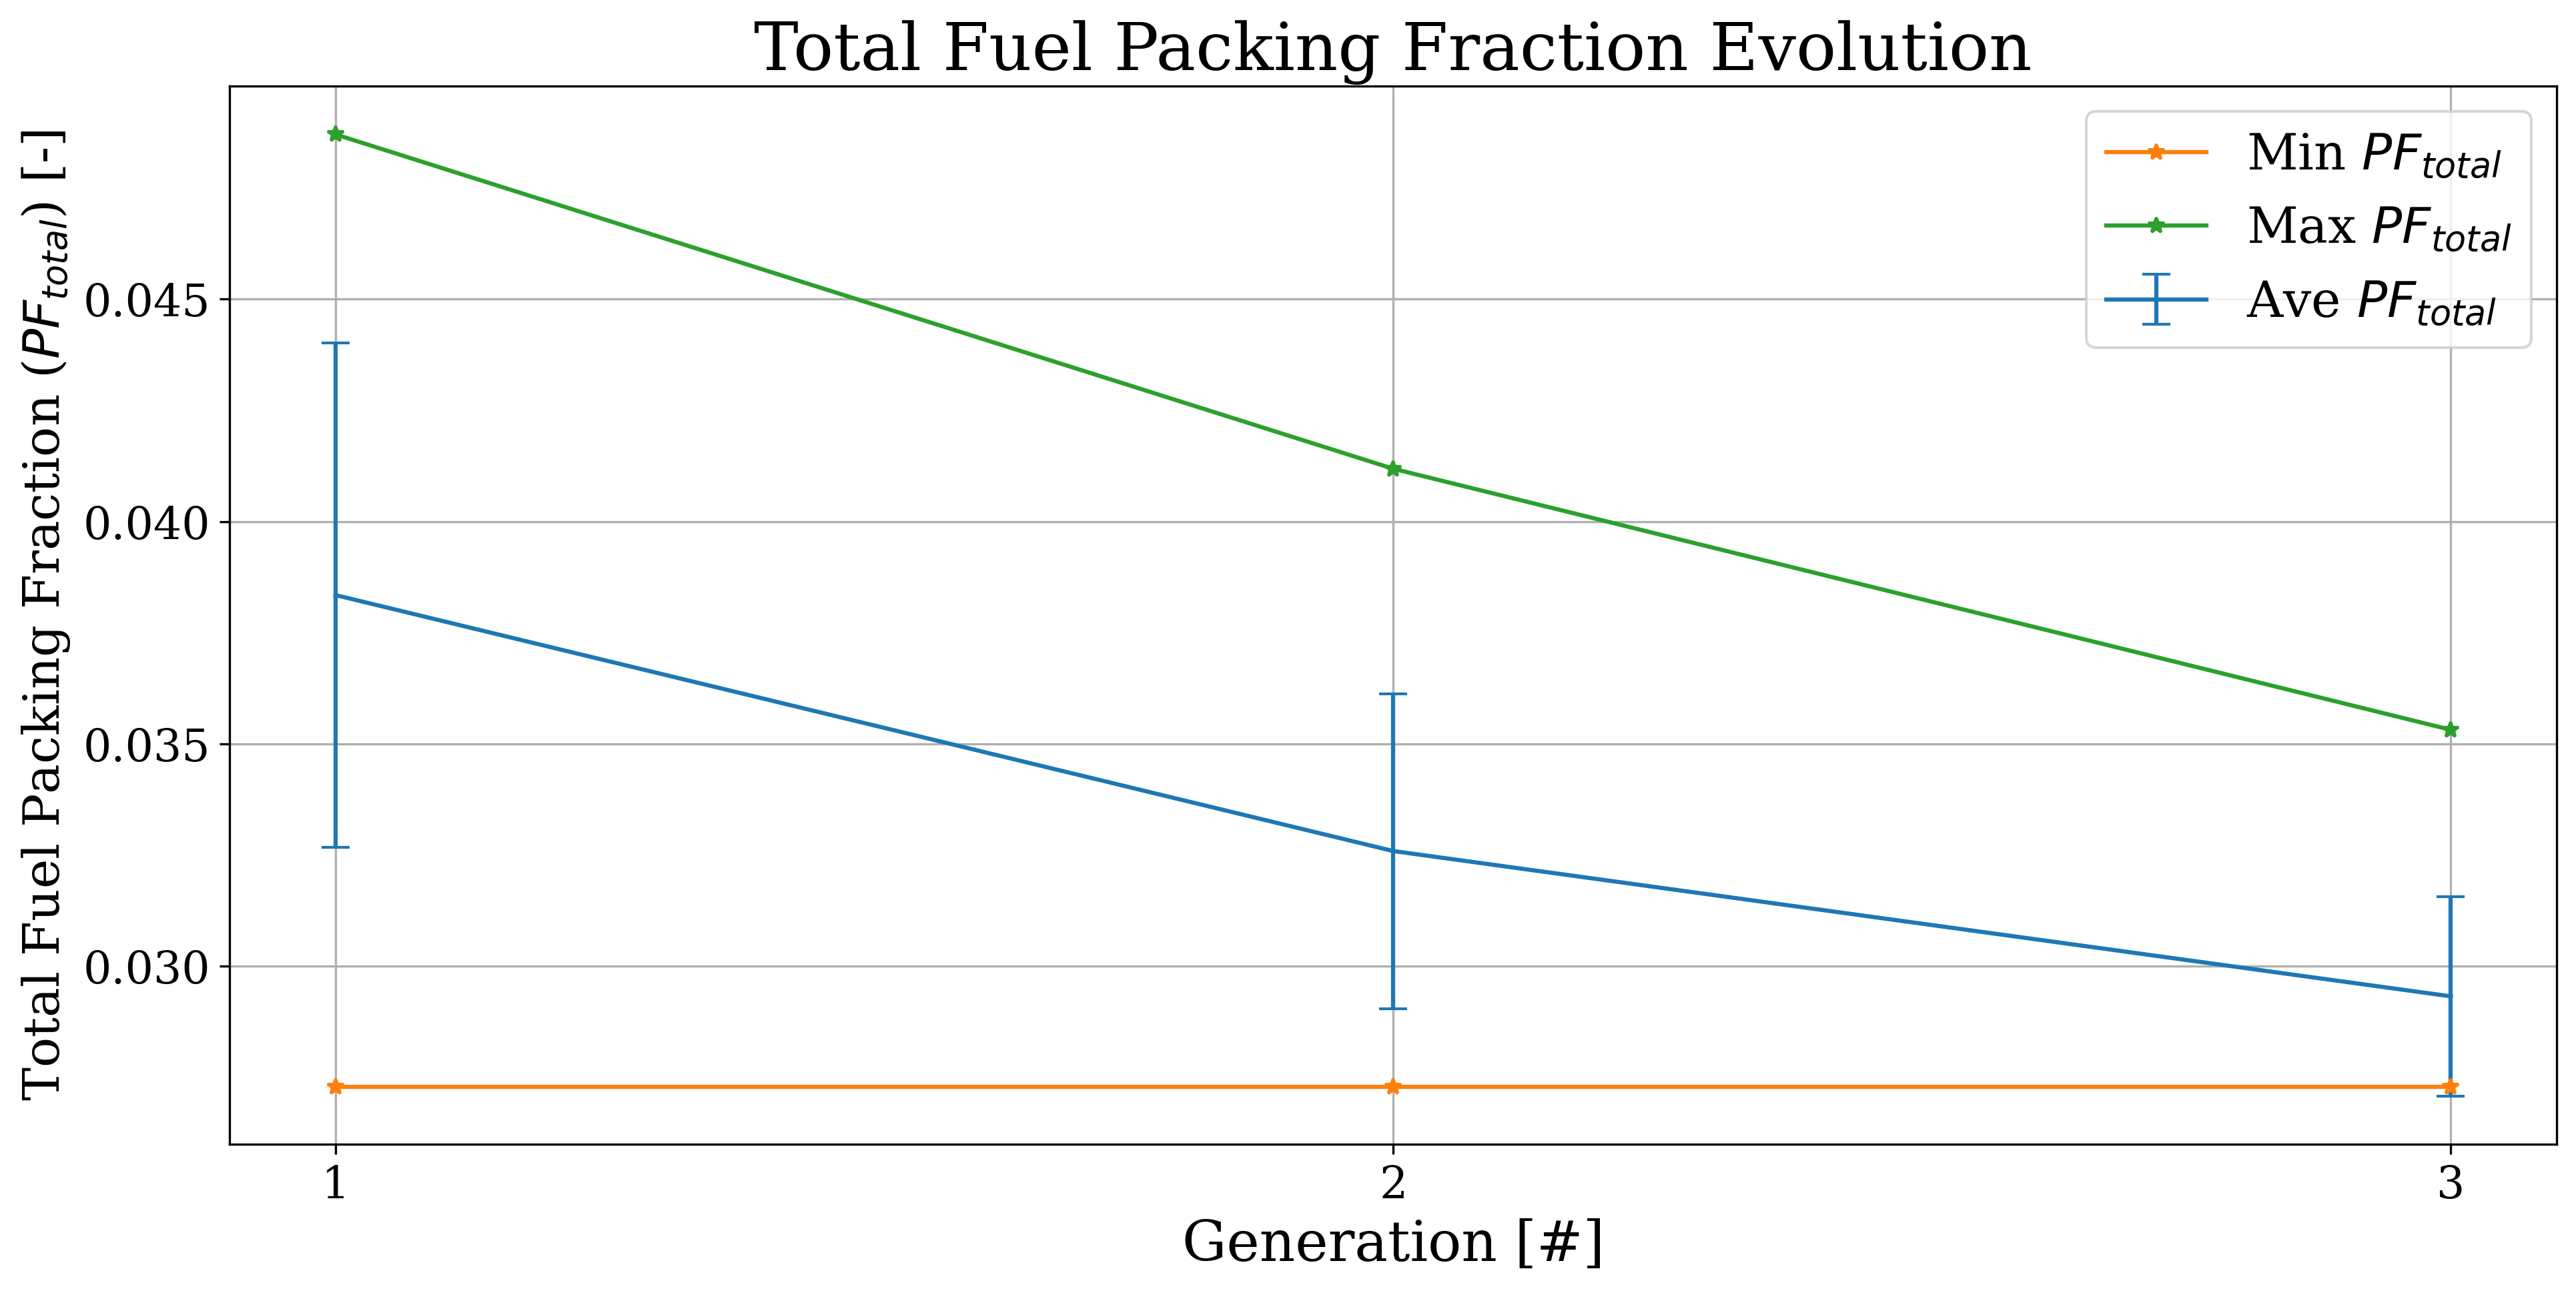
\includegraphics[width=\linewidth]{slab-obj-1-pf-evol-coolant.png}
        \caption{Minimum, average, and maximum total $PF_{total}$ evolution of the 
        population in each generation.}
        \label{fig:slab-obj-1-pf-evol-coolant} 
    \end{subfigure}
    \begin{subfigure}{\textwidth}
        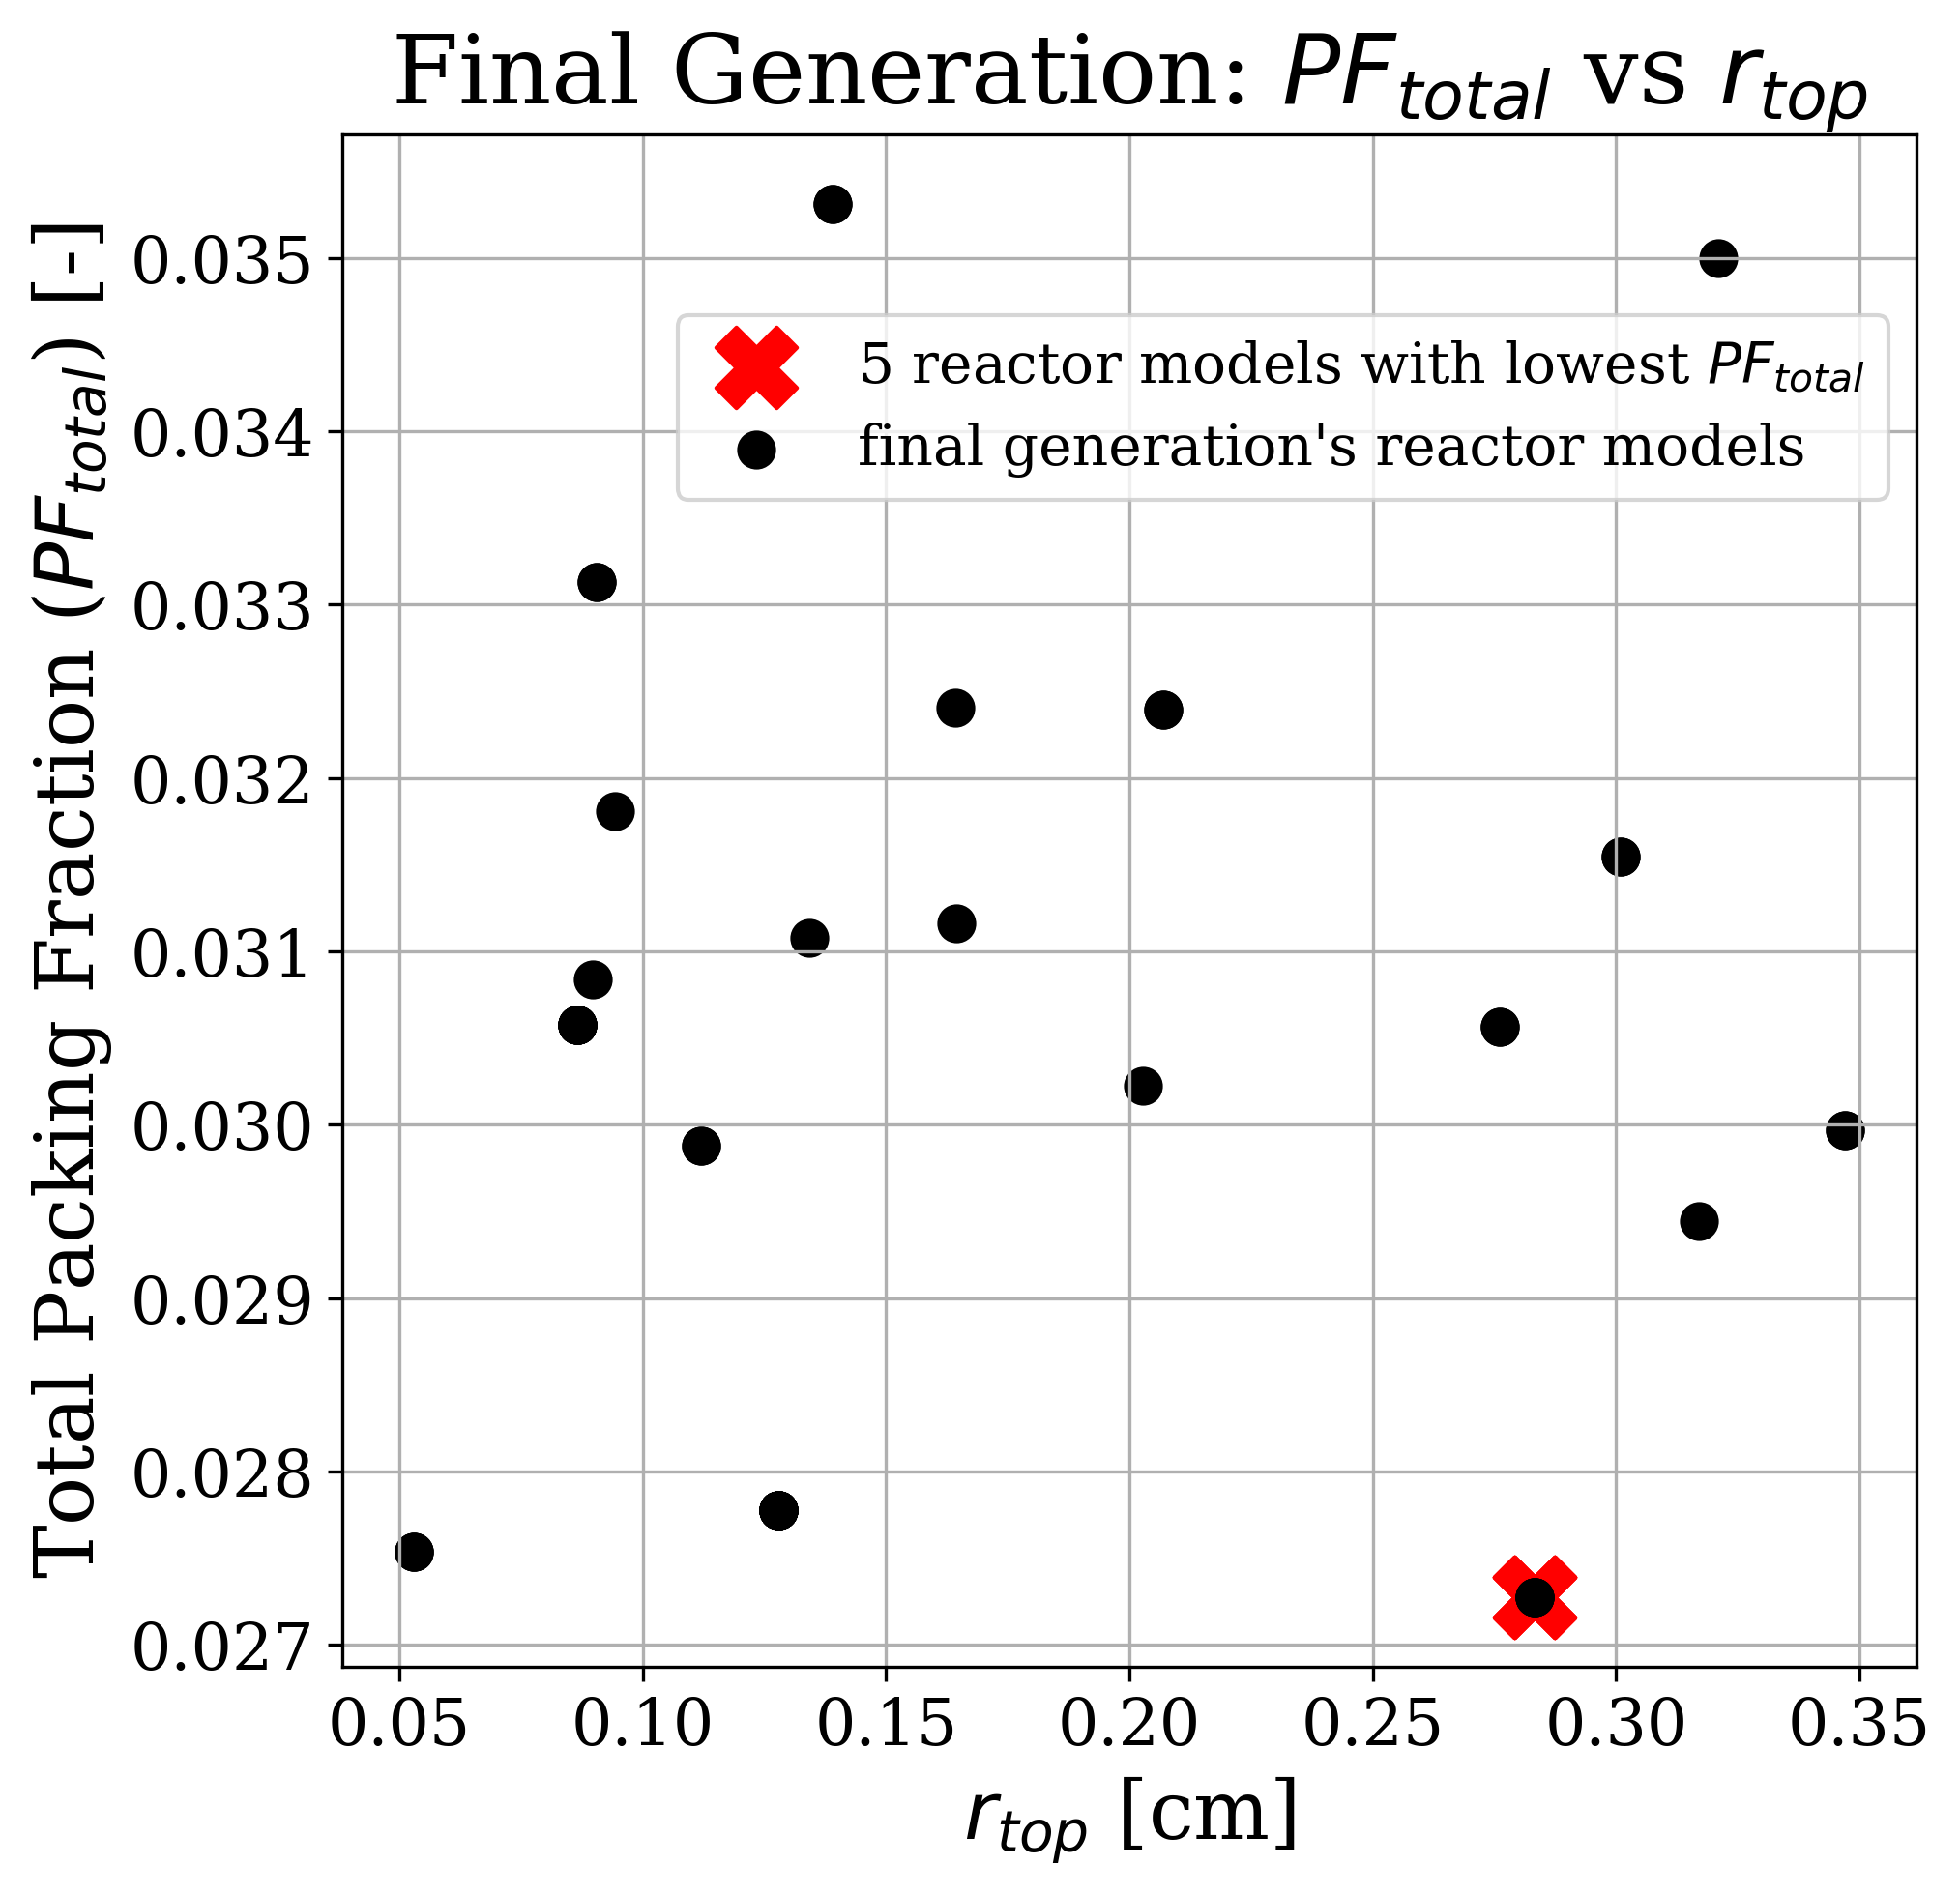
\includegraphics[width=0.49\linewidth]{slab-obj-1-pf-final-coolant-rtop.png}
        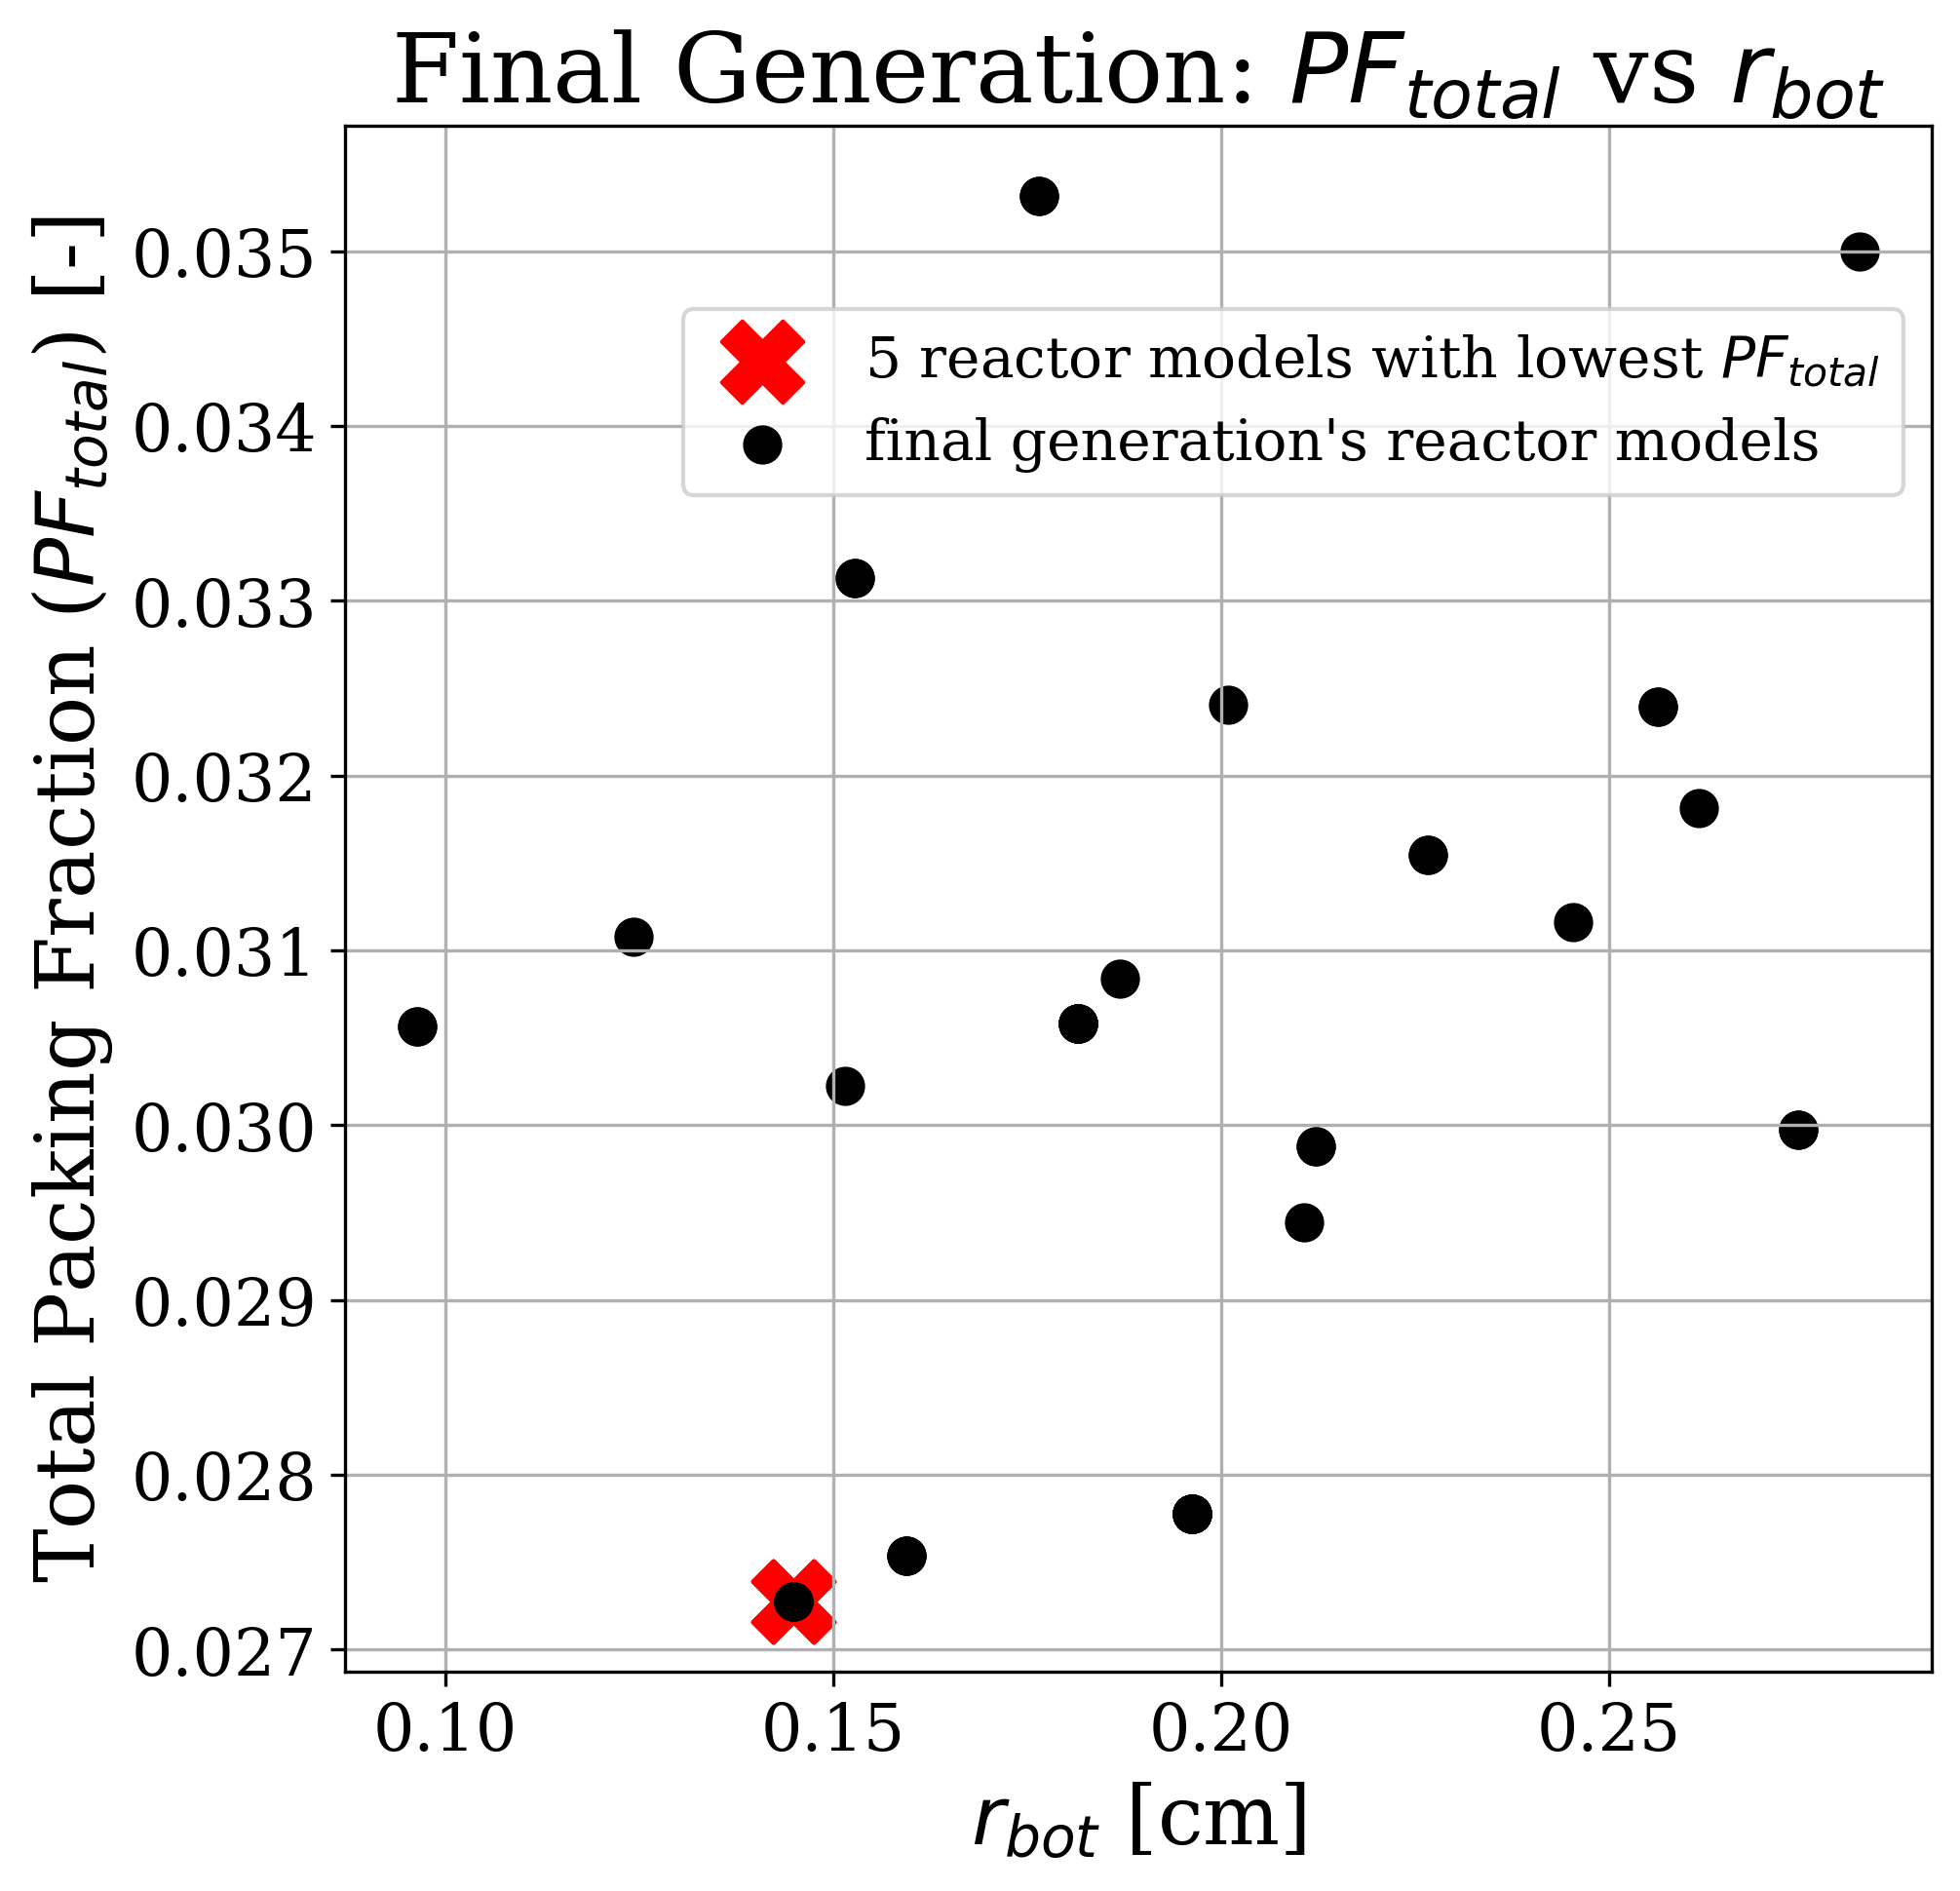
\includegraphics[width=0.49\linewidth]{slab-obj-1-pf-final-coolant-rbot.png}
        \caption{Plots of $r_{top}$ and $r_{bot}$ against $PF_{total}$. 
        Red crosses indicate the five reactor models with the lowest $PF_{total}$.
        The five reactor models with the lowest $PF_{total}$ are the same, thus 
        their crosses overlap.}
        \label{fig:slab-obj-1-pf-final-coolant} 
    \end{subfigure}
    \caption{Simulation p-1d -- ROLLO single-objective optimization to minimize 
    the total fuel packing fraction ($PF_{total}$). 
    Input parameters varied: total fuel packing fraction 
    ($PF_{total}$), and coolant channel shape ($r_{top}, r_{bot}$).}
    \label{fig:slab-obj-1-pf-coolant}
\end{figure}
Figure \ref{fig:slab-obj-1-pf-final-coolant} demonstrates that there is no correlation 
between $PF_{total}$, and $r_{top}$ and $r_{bot}$.

\subsection{Objective: Minimize Maximum Plank Temperature ($T_{max}$)}
\label{sec:plank-1-obj-temp}
This section describes the single-objective p-1b and p-1e optimization simulation
results. 
Both simulations minimize the maximum plank temperature ($T_{max}$) objective. 
The minimize $T_{max}$ objective is important because a reactor that has a lower 
peak tempeature minimizes thermal stresses in the fuel. 
Simulation p-1b varies the \gls{TRISO} packing fraction distribution 
($\rho_{TRISO}(\vec{r})$), while simulation p-1e varies the coolant channel shape. 

\subsubsection{Simulation p-1b: Variation of $\rho_{TRISO}(\vec{r})$}
Table \ref{tab:simulationp1b} summarizes the optimization problem parameters for 
simulation p-1b.  
\begin{table}[htbp!]
    \centering
    \onehalfspacing
    \caption{Simulation p-1b optimization problem parameters.}
	\label{tab:simulationp1b}
    \footnotesize
    \begin{tabular}{l|p{4cm}}
    \hline 
    \multicolumn{2}{c}{\textbf{Single Objective: Simulation p-1b}} \\
    \hline 
    \textbf{Objectives} & Minimize $T_{max}$ \\
    \hline 
    \textbf{Input parameter variations}     
    & $\rho_{TRISO}(\vec{r})$: $0<a<2$ \\
    & $\rho_{TRISO}(\vec{r})$: $0<b<\frac{\pi}{2}$ \\
    & $\rho_{TRISO}(\vec{r})$: $0<c<2\pi$ \\
    \hline
    \textbf{Constraints} & $k_{eff} \geq 1.0$\\ 
    & $PF_{total}$ = 0.0979\\
    \hline 
    \textbf{Genetic algorithm parameters} & Population size: 64 \\
    & Generations: 10 \\
    \hline
    \end{tabular}
\end{table}
Figure \ref{fig:slab-obj-1-temp-evol} shows the plank's $T_{max}$ evolution. 
Figure \ref{fig:slab-obj-1-temp-final} shows the five \gls{TRISO} packing fraction
distributions ($\rho_{TRISO}(\vec{r})$) with the most-minimized $T_{max}$ from the 
final generation. 
Figure \ref{fig:slab-obj-1-temp-most-minimized} illustrates the \gls{AHTR} plank model 
with the most-minimized $T_{max}$. 
\begin{figure}[htbp!]
    \centering
    \begin{subfigure}{0.9\textwidth}
        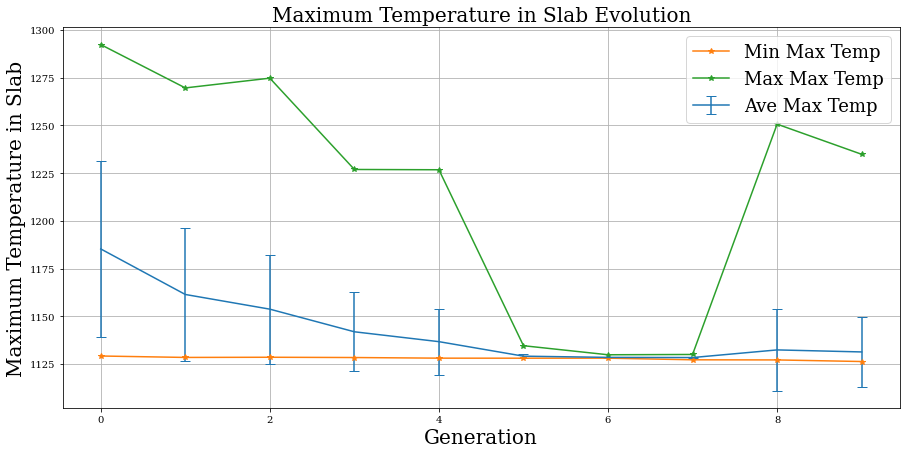
\includegraphics[width=\linewidth]{slab-obj-1-temp-evol.png}
        \caption{Minimum, average, and maximum $T_{max}$ evolution of the 
        population in each generation.}
        \label{fig:slab-obj-1-temp-evol} 
    \end{subfigure}
    \begin{subfigure}{0.9\textwidth}
        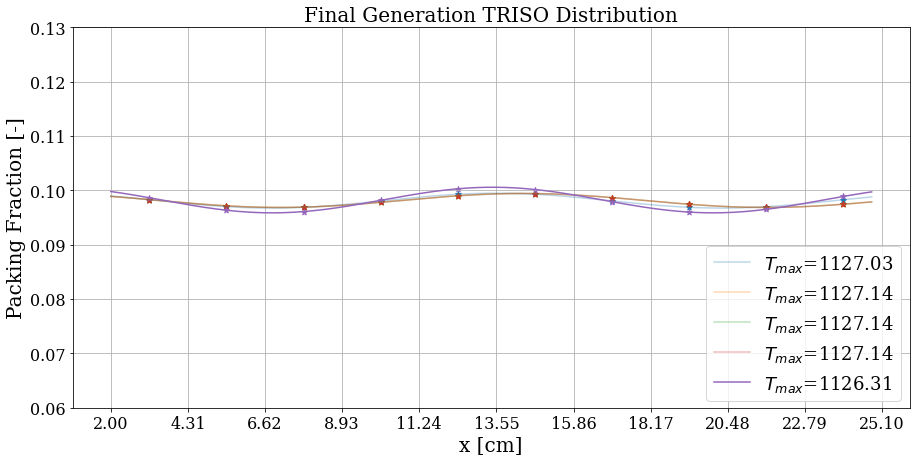
\includegraphics[width=\linewidth]{slab-obj-1-temp-final.png}
        \caption{TRISO distribution for the five reactor models with the 
        lowest AHTR plank $T_{max}$ at the final generation.}
        \label{fig:slab-obj-1-temp-final} 
    \end{subfigure}
    \begin{subfigure}{0.9\textwidth}
        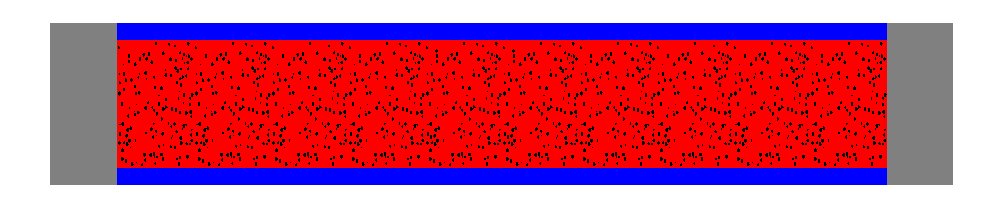
\includegraphics[width=\linewidth]{slab-obj-1-temp-most-minimized.png}
        \caption{\gls{AHTR} plank model with the most-minimized $T_{max}$
        (corresponds to the purple densely dashed distribution in Figure 
        \ref{fig:slab-obj-1-temp-final}).}
        \label{fig:slab-obj-1-temp-most-minimized} 
    \end{subfigure}
    \caption{Simulation p-1b -- ROLLO single-objective optimization to minimize 
    the maximum plank temperature ($T_{max}$). Input parameter varied: TRISO 
    packing fraction distribution ($\rho_{TRISO}(\vec{r})$). $PF_{total}$ = 0.0979.}
    \label{fig:slab-obj-1-temp}
\end{figure}
Figure \ref{fig:slab-obj-1-temp-evol} shows that the minimum and average plank's 
$T_{max}$ converged to approximately 1125 K. 
In Figure \ref{fig:slab-obj-1-temp-final}, a mostly flat TRISO
distribution minimizes $T_{max}$ in the plank; the TRISO distribution 
has two small dips at the one-third and two-third points in the plank 
(6.62cm and 20.48cm). 
Because it is more productive to compare all of the single objective results to one 
another, Section \ref{sec:plank-discussion-single} discusses and explains simulation 
p-1b's most-minimized $T_{max}$ mostly flat TRISO distribution with a packing fraction 
standard deviation of $0.0015$. 

\subsubsection{Simulation p-1e: Variation of Coolant Channel Shape}
Table \ref{tab:simulationp1e} summarizes the optimization problem parameters for 
simulation p-1e.  
\begin{table}[htbp!]
    \centering
    \onehalfspacing
    \caption{Simulation p-1e optimization problem parameters.}
	\label{tab:simulationp1e}
    \footnotesize
    \begin{tabular}{l|p{6.5cm}}
    \hline 
    \multicolumn{2}{c}{\textbf{Single Objective: Simulation p-1e}} \\
    \hline 
    \textbf{Objectives} & Minimize $T_{max}$ \\
    \hline 
    \textbf{Input parameter variations} 
    & Coolant channel shape: $0.05<r_{top}<0.35$ \\
    & Coolant channel shape: $0.05<r_{bot}<0.35$ \\
    \hline
    \textbf{Constraints} & $k_{eff} \geq 1.35$\\ 
    & $PF_{total}$ = 0.0979\\
    \hline 
    \textbf{Genetic algorithm parameters} & Population size: 64 \\
    & Generations: 4 \\
    \hline
    \end{tabular}
\end{table}
Figure \ref{fig:slab-obj-1-temp-evol-coolant} shows the plank's $T_{max}$ evolution.
Figure \ref{fig:slab-obj-1-temp-final-coolant} shows the plots of $r_{top}$ and 
$r_{bot}$ against $T_{max}$.
Figure \ref{fig:slab-obj-1-temp-most-minimized-coolant} illustrates the \gls{AHTR} 
plank model with the most-minimized $T_{max}$. 
\begin{figure}[htbp!]
    \centering
    \begin{subfigure}{\textwidth}
        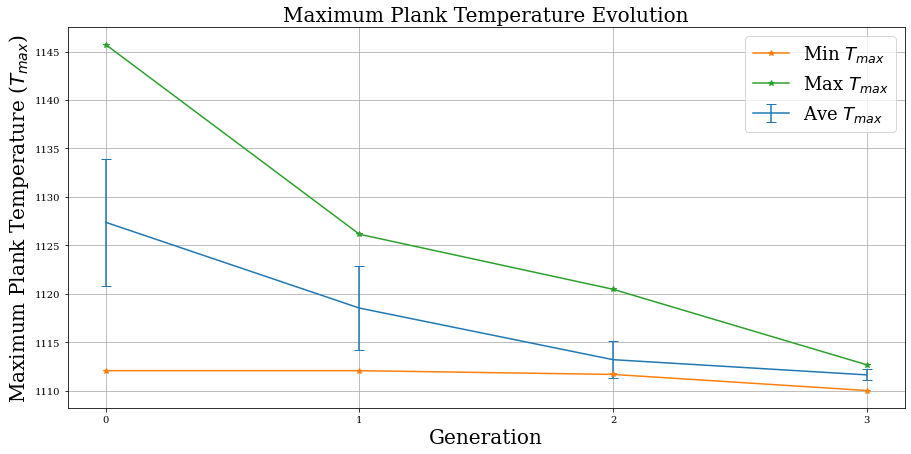
\includegraphics[width=\linewidth]{slab-obj-1-temp-evol-coolant.png}
        \caption{Minimum, average, and maximum $T_{max}$ evolution of the 
        population in each generation.}
        \label{fig:slab-obj-1-temp-evol-coolant} 
    \end{subfigure}
    \begin{subfigure}{\textwidth}
        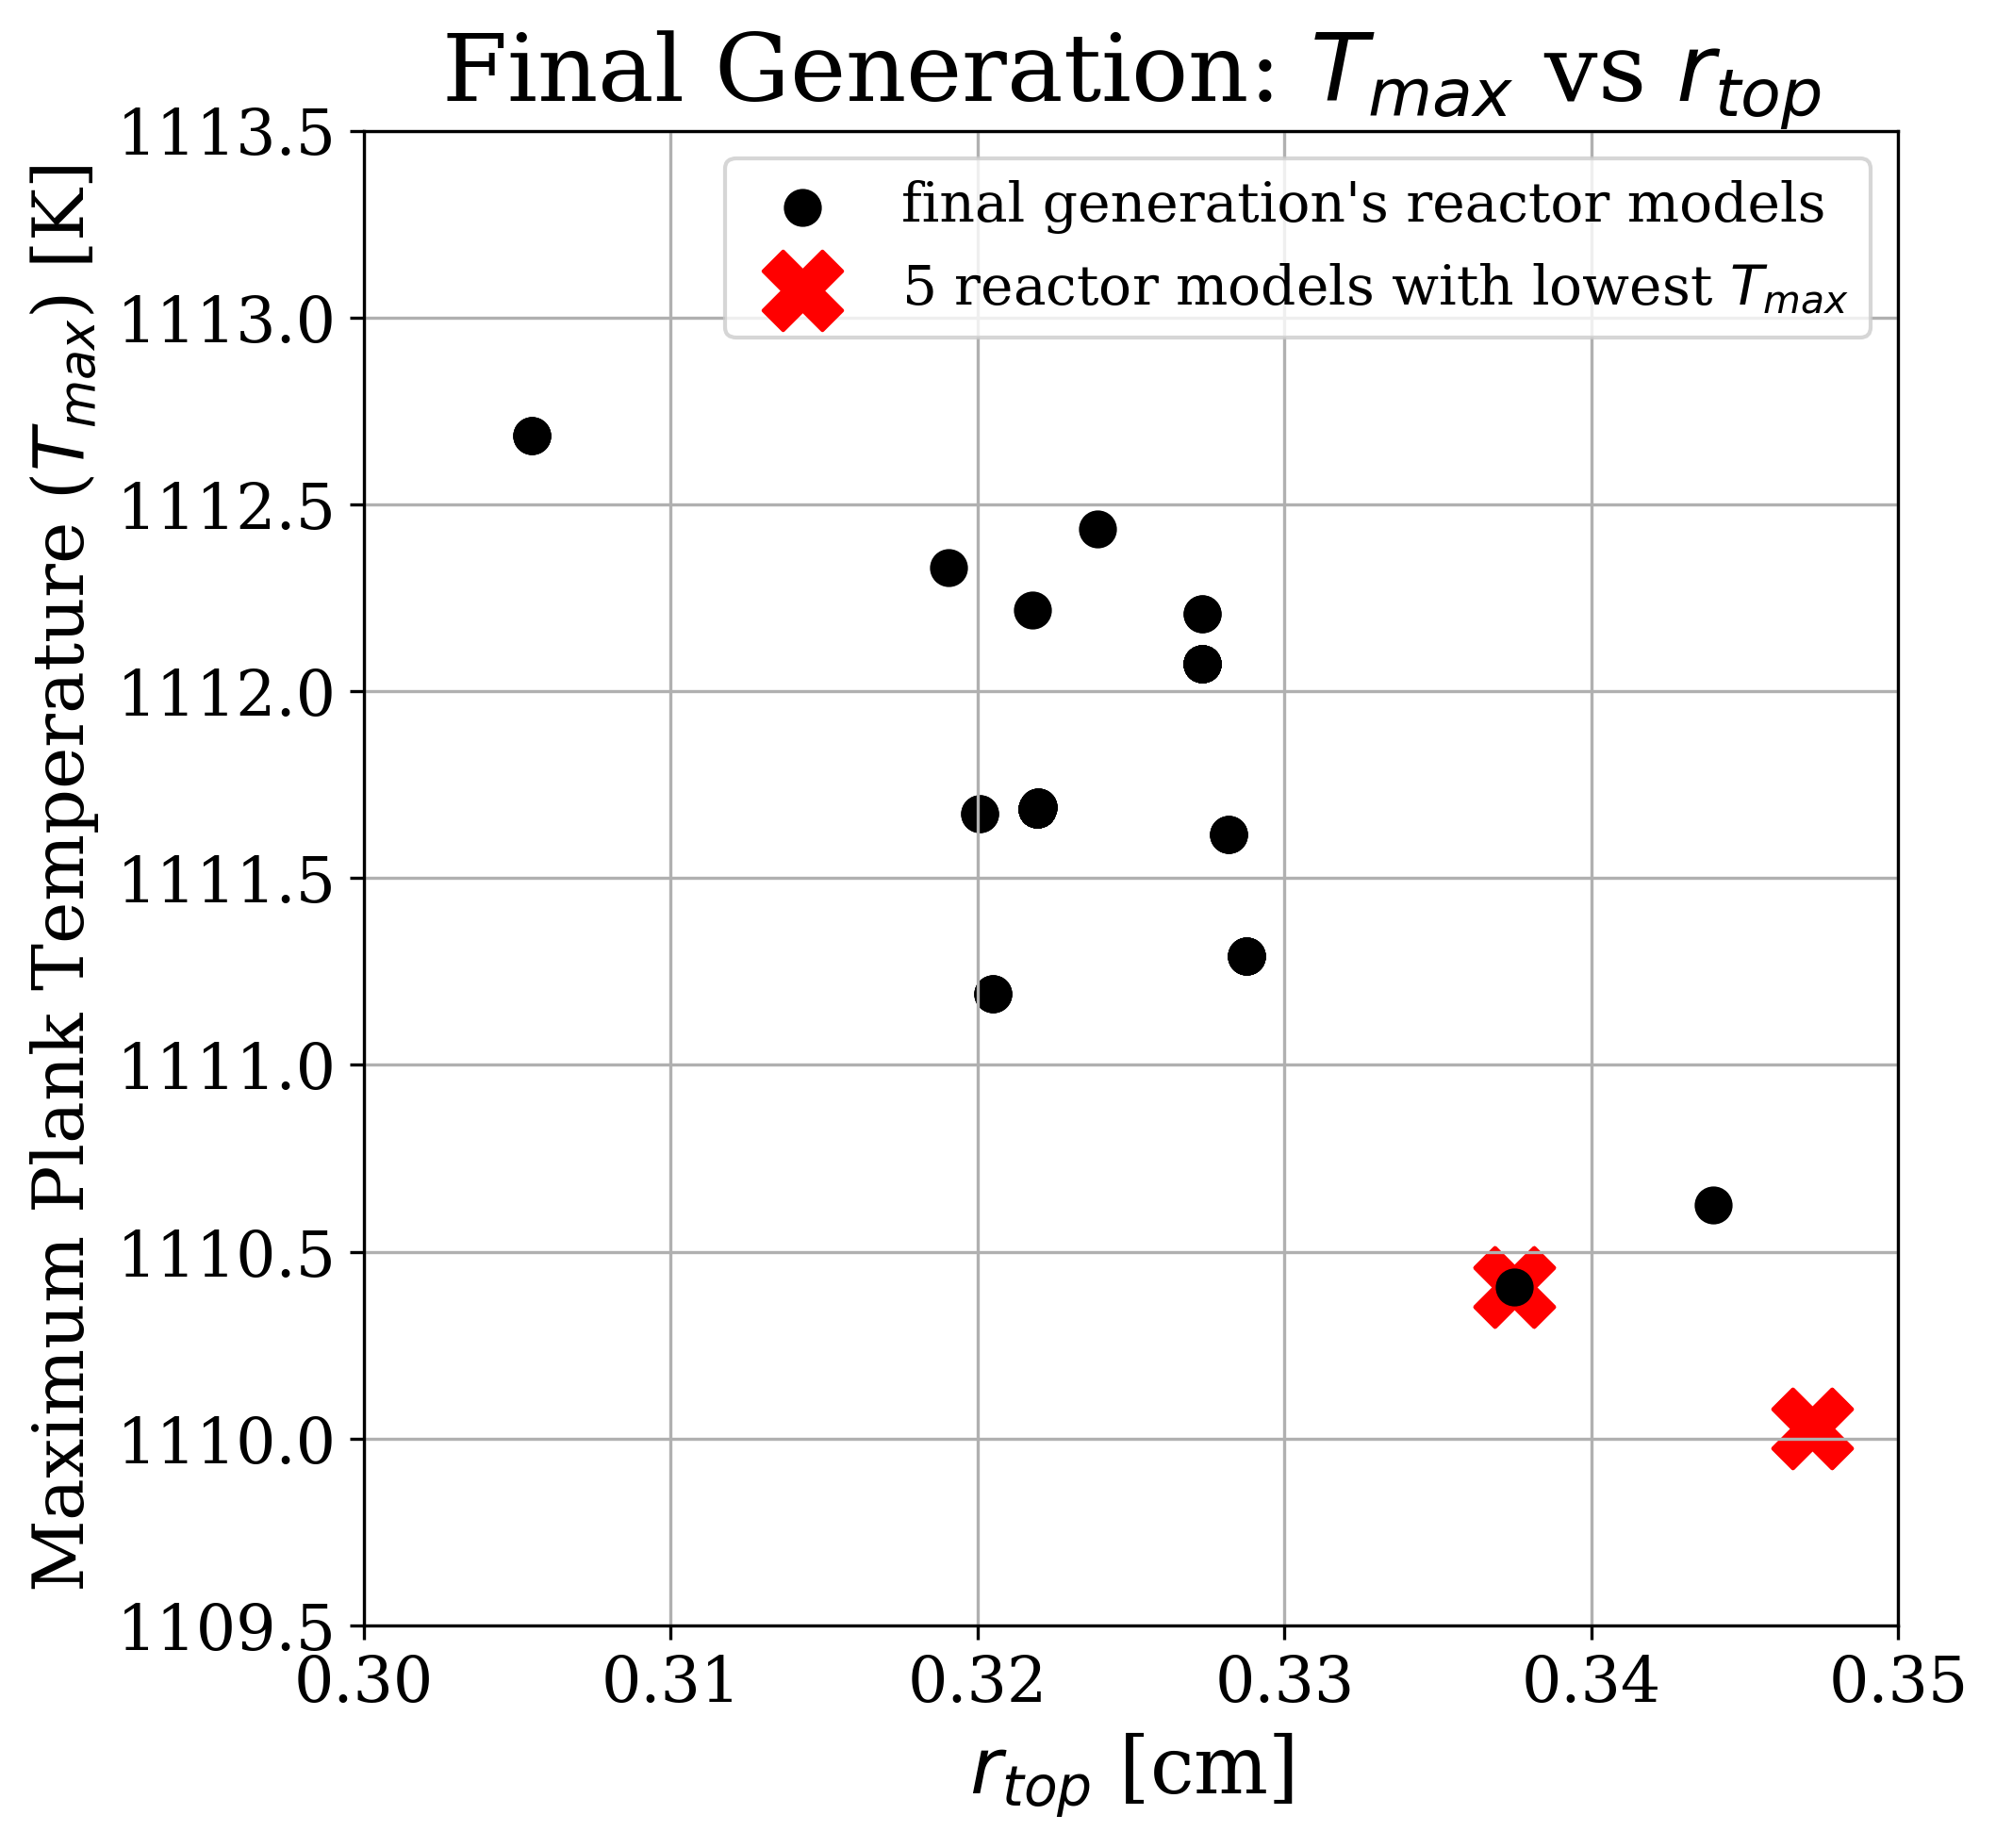
\includegraphics[width=0.49\linewidth]{slab-obj-1-temp-final-coolant-rtop.png}
        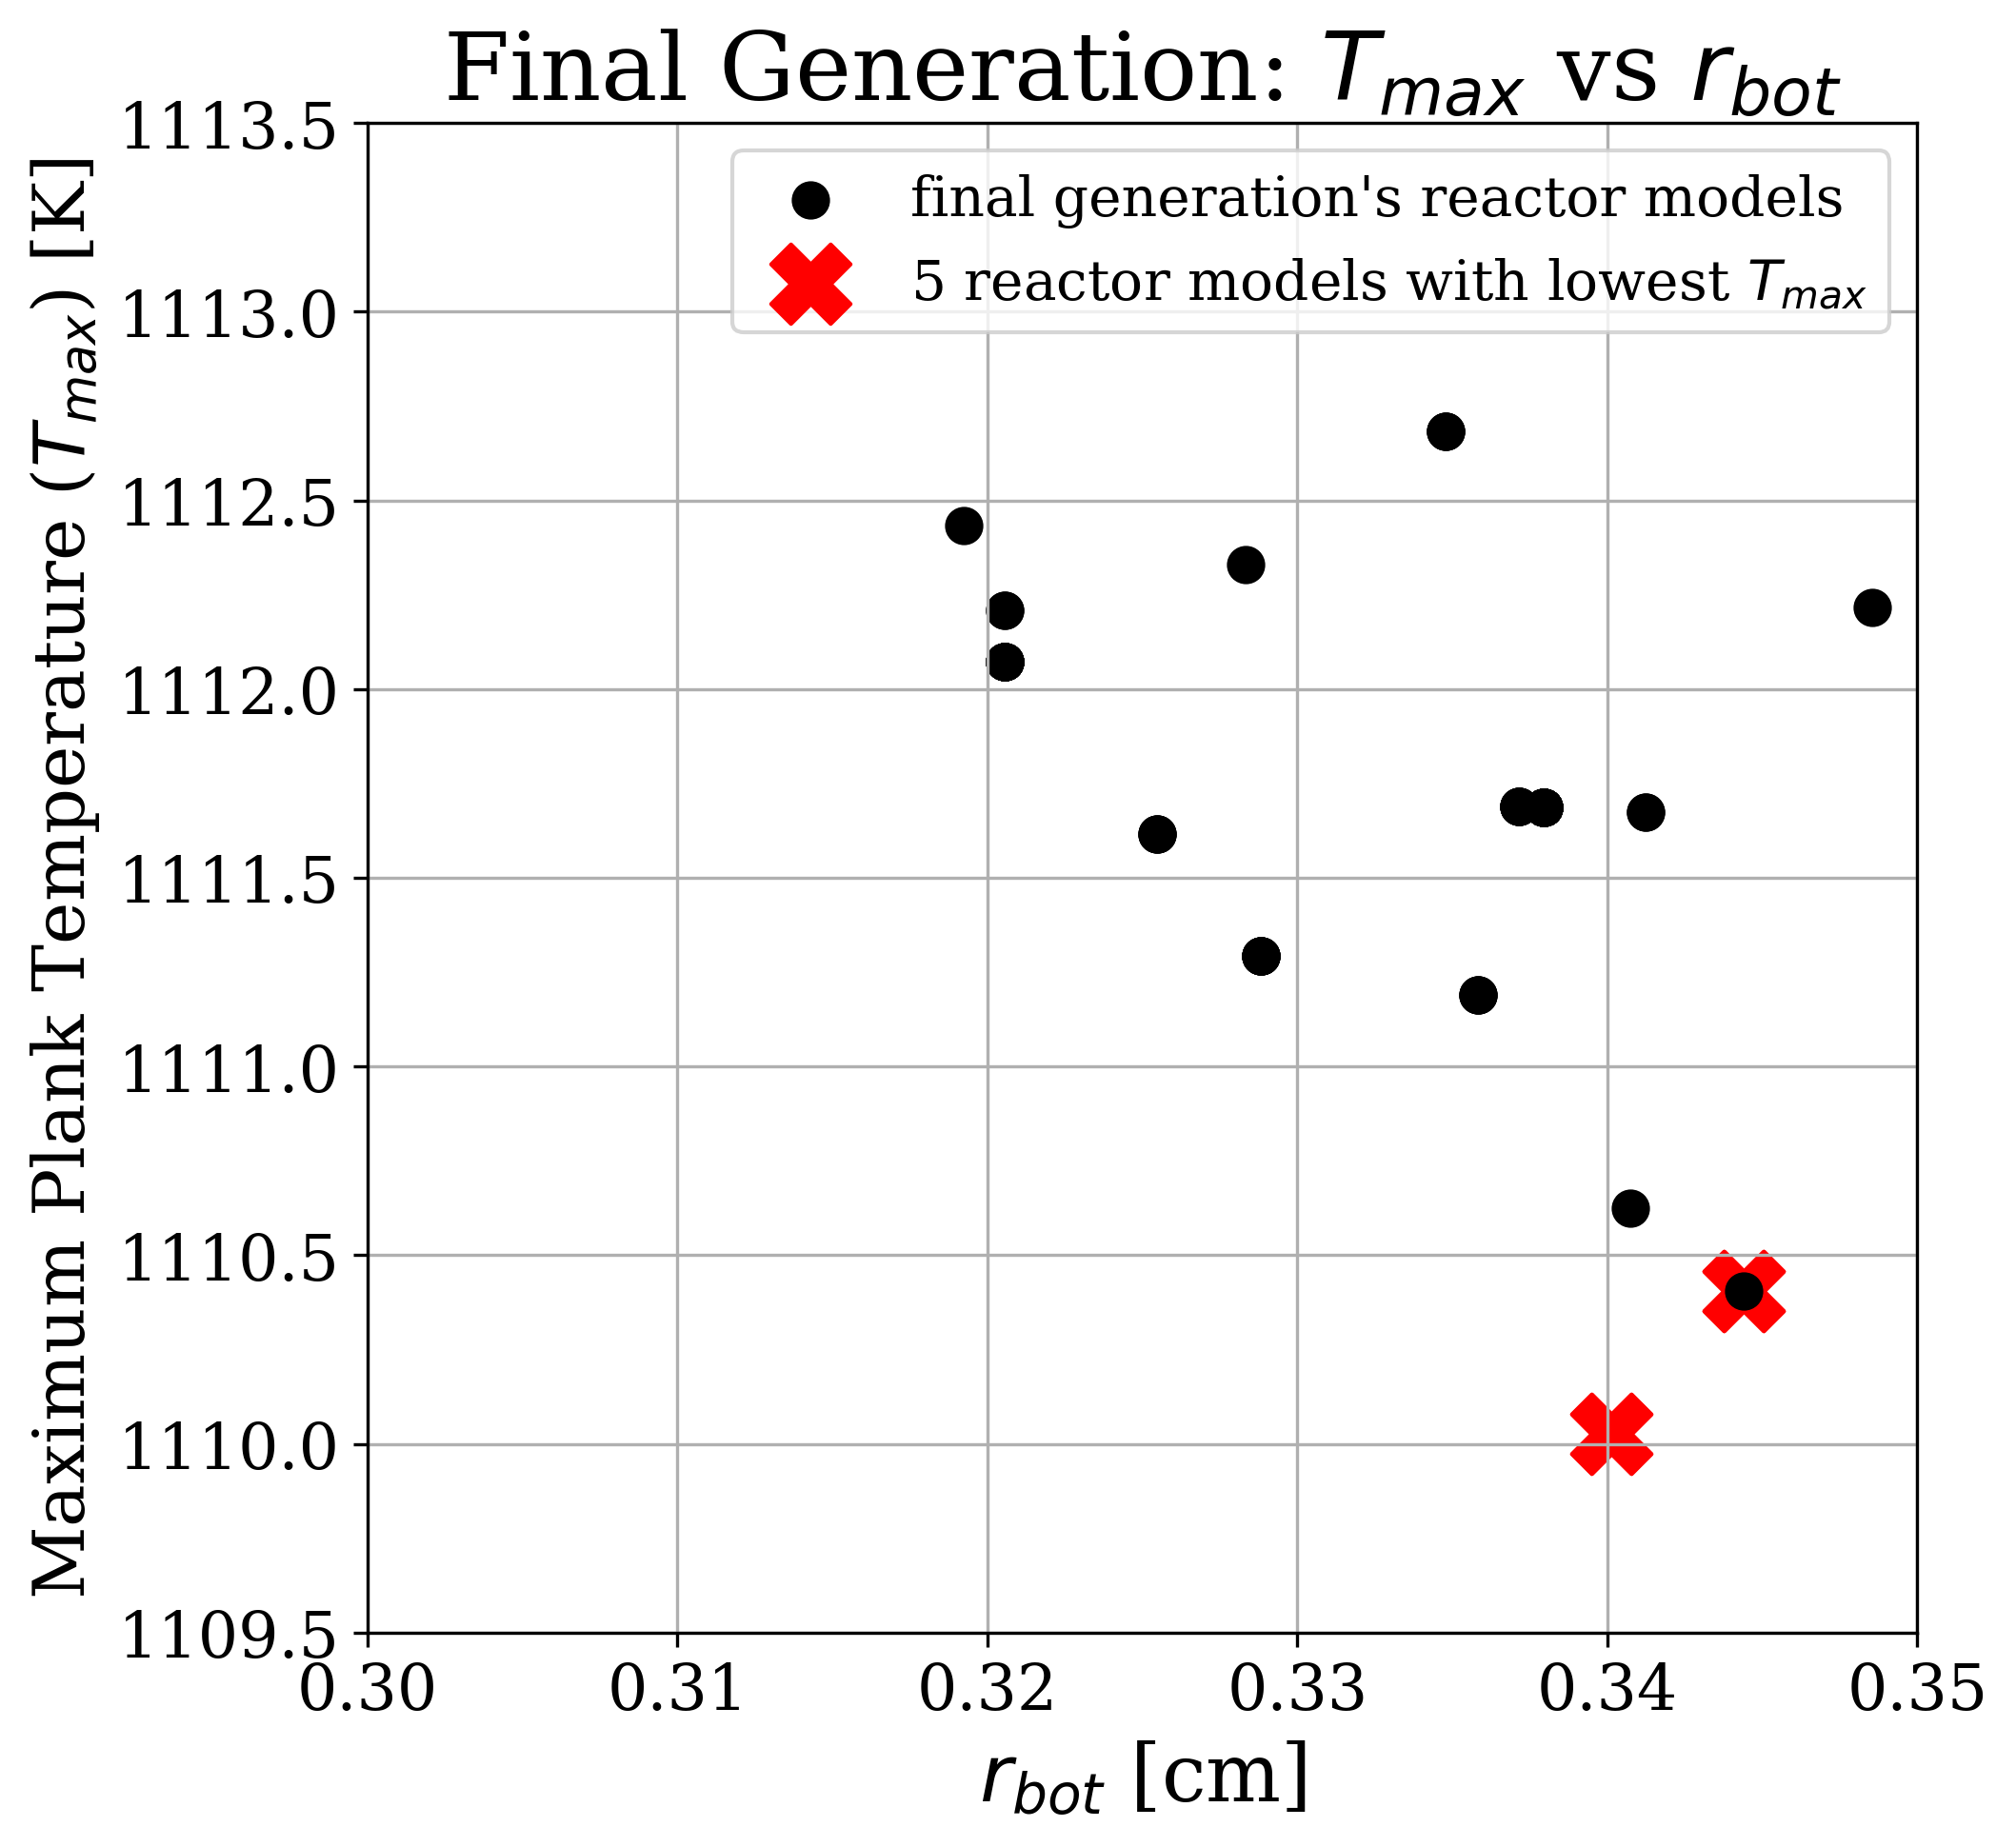
\includegraphics[width=0.49\linewidth]{slab-obj-1-temp-final-coolant-rbot.png}
        \caption{Plots of $r_{top}$ and $r_{bot}$ against $T_{max}$. 
        Red crosses indicate the five reactor models with the 
        lowest $T_{max}$.
        Some of the five reactor models with the lowest $T_{max}$ are the same, thus 
        their crosses overlap.}
        \label{fig:slab-obj-1-temp-final-coolant} 
    \end{subfigure}
    \begin{subfigure}{\textwidth}
        
\includegraphics[width=\linewidth]{slab-obj-1-temp-most-minimized-coolant.png}
        \caption{\gls{AHTR} plank model with the most-minimized $T_{max}$. 
        $r_{top} = 0.337$ and $r_{bot} = 0.344$.}
        \label{fig:slab-obj-1-temp-most-minimized-coolant} 
    \end{subfigure}
    \caption{Simulation p-1e -- ROLLO single-objective optimization to minimize 
    the maximum plank temperature ($T_{max}$). 
    Input parameters varied: $r_{top}, r_{bot}$. $PF_{total}$ = 0.0979 and constant 
    TRISO distribution.}
    \label{fig:slab-obj-1-temp-coolant}
\end{figure}
Figure \ref{fig:slab-obj-1-temp-final-coolant} demonstrates a negative 
linear correlation between the plank's $T_{max}$, and $r_{top}$ and $r_{bot}$.
Section \ref{sec:plank-discussion-single} discusses and explains the relationship 
between $T_{max}$ and coolant channel shape. 

\subsection{Objective: Minimize Fuel-Normalized Power Peaking Factor ($PPF_{fuel}$)}
\label{sec:plank-1-obj-ppf}
This section describes the single-objective p-1c and p-1f optimization simulation
results. 
Both simulations minimize fuel-normalized power peaking factor ($PPF_{fuel}$). 
The minimize $PPF_{fuel}$ objective is important because a reactor that has a lower 
fuel-normalized power peaking factor will have more even and efficient fuel utilization. 
Simulation p-1c varies the \gls{TRISO} packing fraction distribution 
($\rho_{TRISO}(\vec{r})$), while simulation p-1f varies the coolant channel shape. 

\subsubsection{Simulation p-1c: Variation of $\rho_{TRISO}(\vec{r})$}
Table \ref{tab:simulationp1c} shows simulation p-1c's optimization problem parameters. 
\begin{table}[htbp!]
    \centering
    \onehalfspacing
    \caption{Simulation p-1c optimization problem parameters.}
	\label{tab:simulationp1c}
    \footnotesize
    \begin{tabular}{l|p{4cm}}
    \hline 
    \multicolumn{2}{c}{\textbf{Single Objective: Simulation p-1c}} \\
    \hline 
    \textbf{Objectives} & Minimize $PPF_{fuel}$ \\
    \hline 
    \textbf{Input parameter variations}
    & $\rho_{TRISO}(\vec{r})$: $0<a<2$ \\
    & $\rho_{TRISO}(\vec{r})$: $0<b<\frac{\pi}{2}$ \\
    & $\rho_{TRISO}(\vec{r})$: $0<c<2\pi$ \\
    \hline
    \textbf{Constraints} & $k_{eff} \geq 1.0$\\ 
    & $PF_{total}$ = 0.0979\\
    \hline 
    \textbf{Genetic algorithm parameters} & Population size: 60 \\
    & Generations: 10 \\
    \hline
    \end{tabular}
\end{table}
Figure \ref{fig:slab-obj-1-ppf-evol} shows the plank's $PPF_{fuel}$ evolution 
converges over ten generations.  
Figure \ref{fig:slab-obj-1-ppf-final} shows the five overlapped \gls{TRISO} 
packing fraction distributions ($\rho_{TRISO}(\vec{r})$) in the final generation 
with the most-minimized $PPF_{fuel}$. 
Figure \ref{fig:slab-obj-1-ppf-most-minimized} illustrates the \gls{AHTR} plank model 
with the most-minimized $PPF_{fuel}$. 
\begin{figure}[htbp!]
    \centering
    \begin{subfigure}{0.9\textwidth}
        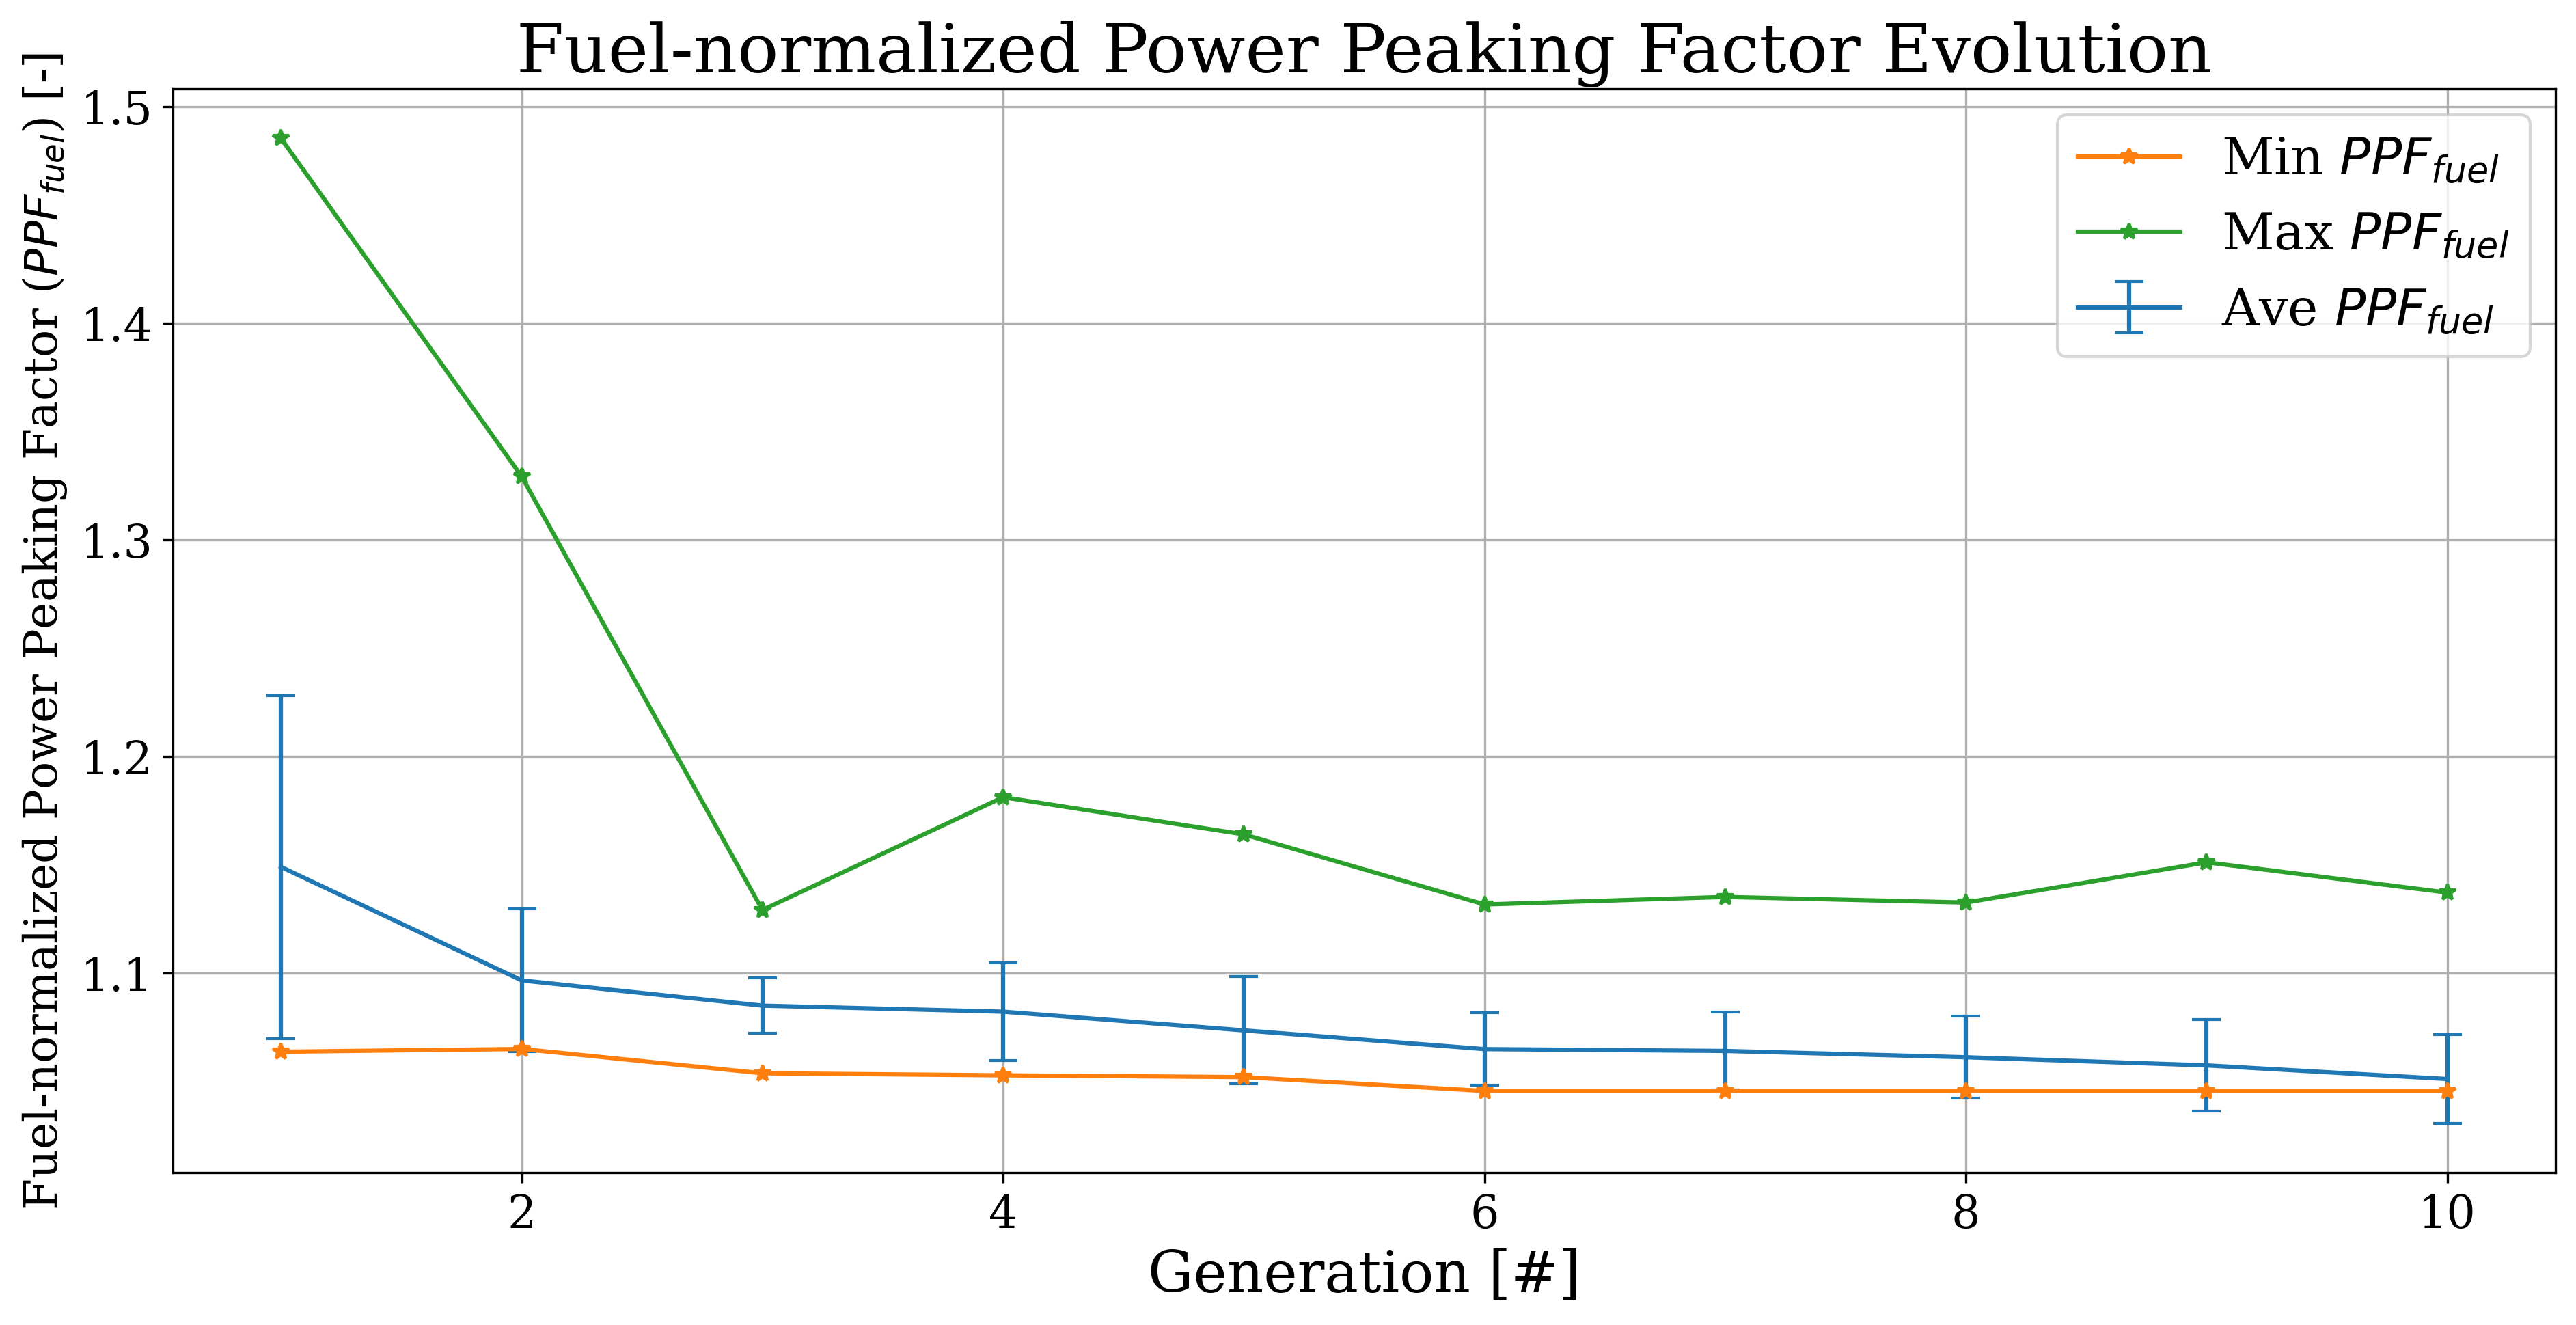
\includegraphics[width=\linewidth]{slab-obj-1-ppf-evol.png}
        \caption{Minimum, average, and maximum $PPF_{fuel}$ evolution of the 
        population in each generation.}
        \label{fig:slab-obj-1-ppf-evol} 
    \end{subfigure}
    \begin{subfigure}{0.9\textwidth}
        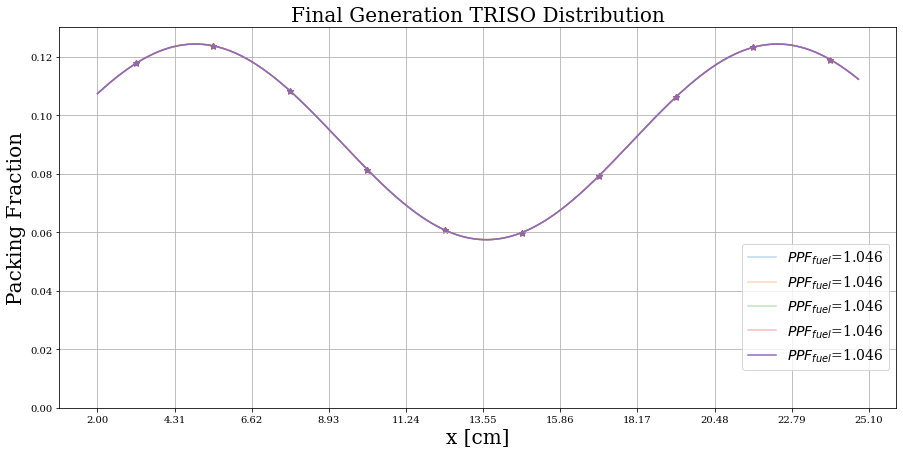
\includegraphics[width=\linewidth]{slab-obj-1-ppf-final.png}
        \caption{TRISO distribution for the five reactor models with the 
        lowest $PPF_{fuel}$ in the AHTR plank at the final generation.}
        \label{fig:slab-obj-1-ppf-final} 
    \end{subfigure}
    \begin{subfigure}{0.9\textwidth}
        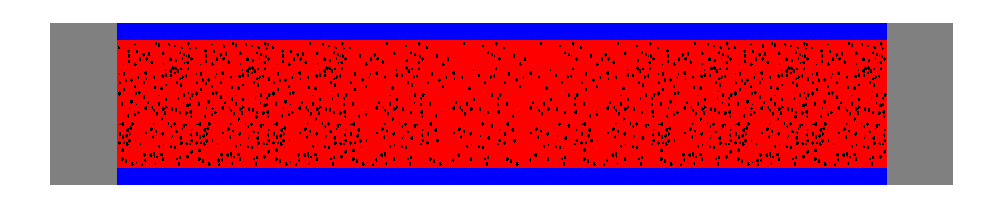
\includegraphics[width=\linewidth]{slab-obj-1-ppf-most-minimized.png}
        \caption{\gls{AHTR} plank model with the most-minimized $PPF_{fuel}$
        (corresponds to the purple densely dashed distribution in Figure 
        \ref{fig:slab-obj-1-ppf-final}).
        The five reactor models with the lowest $PPF_{fuel}$ are the same, thus 
        their lines overlap.}
        \label{fig:slab-obj-1-ppf-most-minimized} 
    \end{subfigure}
    \caption{Simulation p-1c -- ROLLO single-objective optimization to minimize 
    AHTR plank's fuel-normalized power peaking factor ($PPF_{fuel}$). 
    Input parameters varied: TRISO distribution ($\rho_{TRISO}(\vec{r})$).
    $PF_{total}$ = 0.0979.}
    \label{fig:slab-obj-1-ppf}
\end{figure}
In Figure \ref{fig:slab-obj-1-ppf-final}, the plank model with the most-minimized 
$PPF_{fuel}$ has a TRISO distribution that peaks near the edges of the fuel region and 
has a minimum point at the plank's center.
Section \ref{sec:plank-discussion-single} discusses the driving factors for the minimize 
$PPF_{fuel}$ objective and explains simulation p-1c's most-minimized $PPF_{fuel}$ 
TRISO distribution. 

\subsubsection{Simulation p-1f: Variation of Coolant Channel Shape}
Table \ref{tab:simulationp1f} shows simulation p-1f's optimization problem parameters. 
\begin{table}[htbp!]
    \centering
    \onehalfspacing
    \caption{Simulation p-1f optimization problem parameters.}
	\label{tab:simulationp1f}
    \footnotesize
    \begin{tabular}{l|p{6.5cm}}
    \hline 
    \multicolumn{2}{c}{\textbf{Single Objective: Simulation p-1f}} \\
    \hline 
    \textbf{Objectives} & Minimize $PPF_{fuel}$ \\
    \hline 
    \textbf{Input parameter variations} 
    & Coolant channel shape: $0.05<r_{top}<0.35$ \\
    & Coolant channel shape: $0.05<r_{bot}<0.35$ \\
    \hline
    \textbf{Constraints} & $k_{eff} \geq 1.35$\\ 
    & $PF_{total}$ = 0.0979\\
    \hline 
    \textbf{Genetic algorithm parameters} & Population size: 64 \\
    & Generations: 5 \\
    \hline
    \end{tabular}
\end{table}
Figure \ref{fig:slab-obj-1-ppf-evol-coolant} shows the plank's $PPF_{fuel}$ evolution, 
and Figure \ref{fig:slab-obj-1-ppf-final-coolant} shows the plots $r_{top}$ and 
$r_{bot}$ against $PPF_{fuel}$. 
\begin{figure}[htbp!]
    \centering
    \begin{subfigure}{\textwidth}
        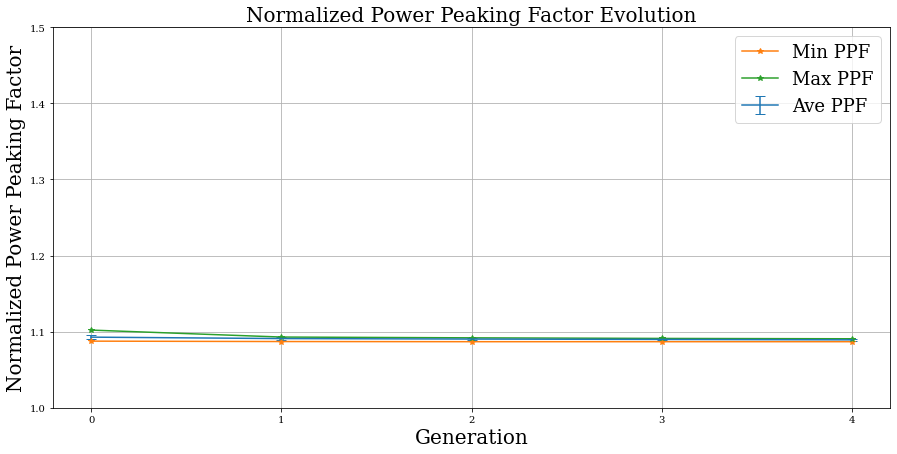
\includegraphics[width=\linewidth]{slab-obj-1-ppf-evol-coolant.png}
        \caption{Minimum, average, and maximum $PPF_{fuel}$ evolution of the 
        population in each generation.}
        \label{fig:slab-obj-1-ppf-evol-coolant} 
    \end{subfigure}
    \begin{subfigure}{\textwidth}
        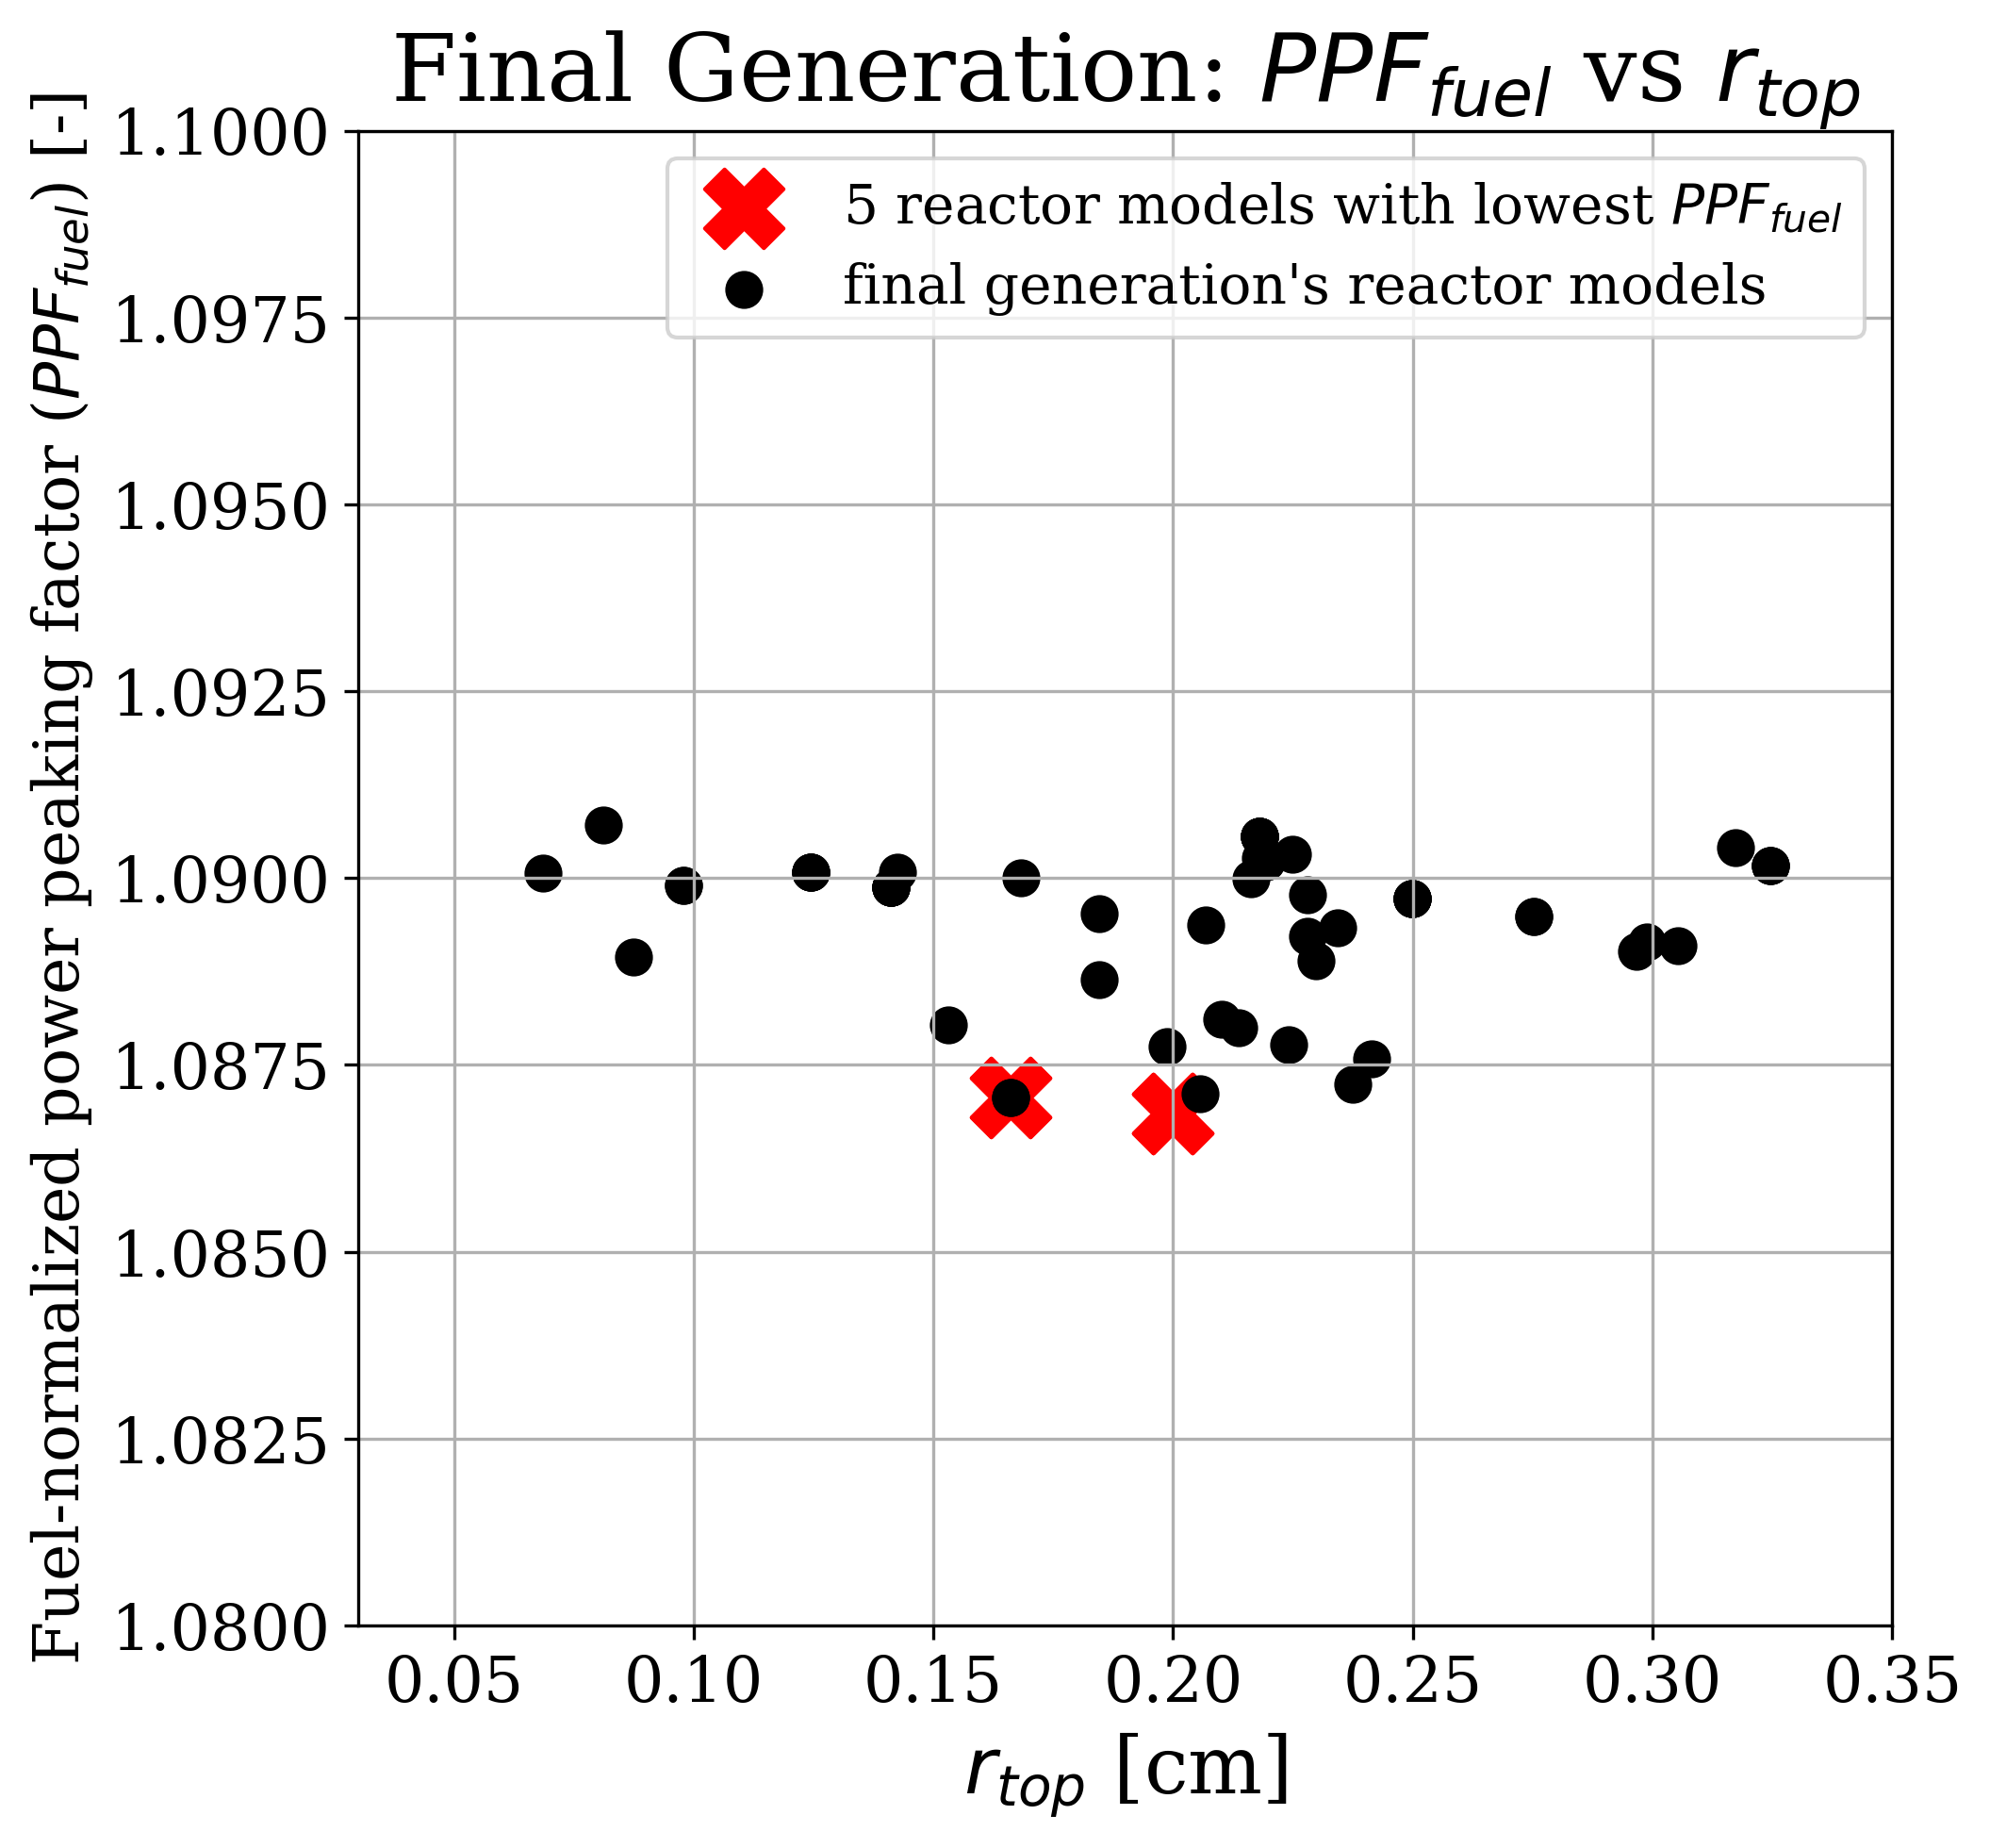
\includegraphics[width=0.49\linewidth]{slab-obj-1-ppf-final-coolant-rtop.png}
        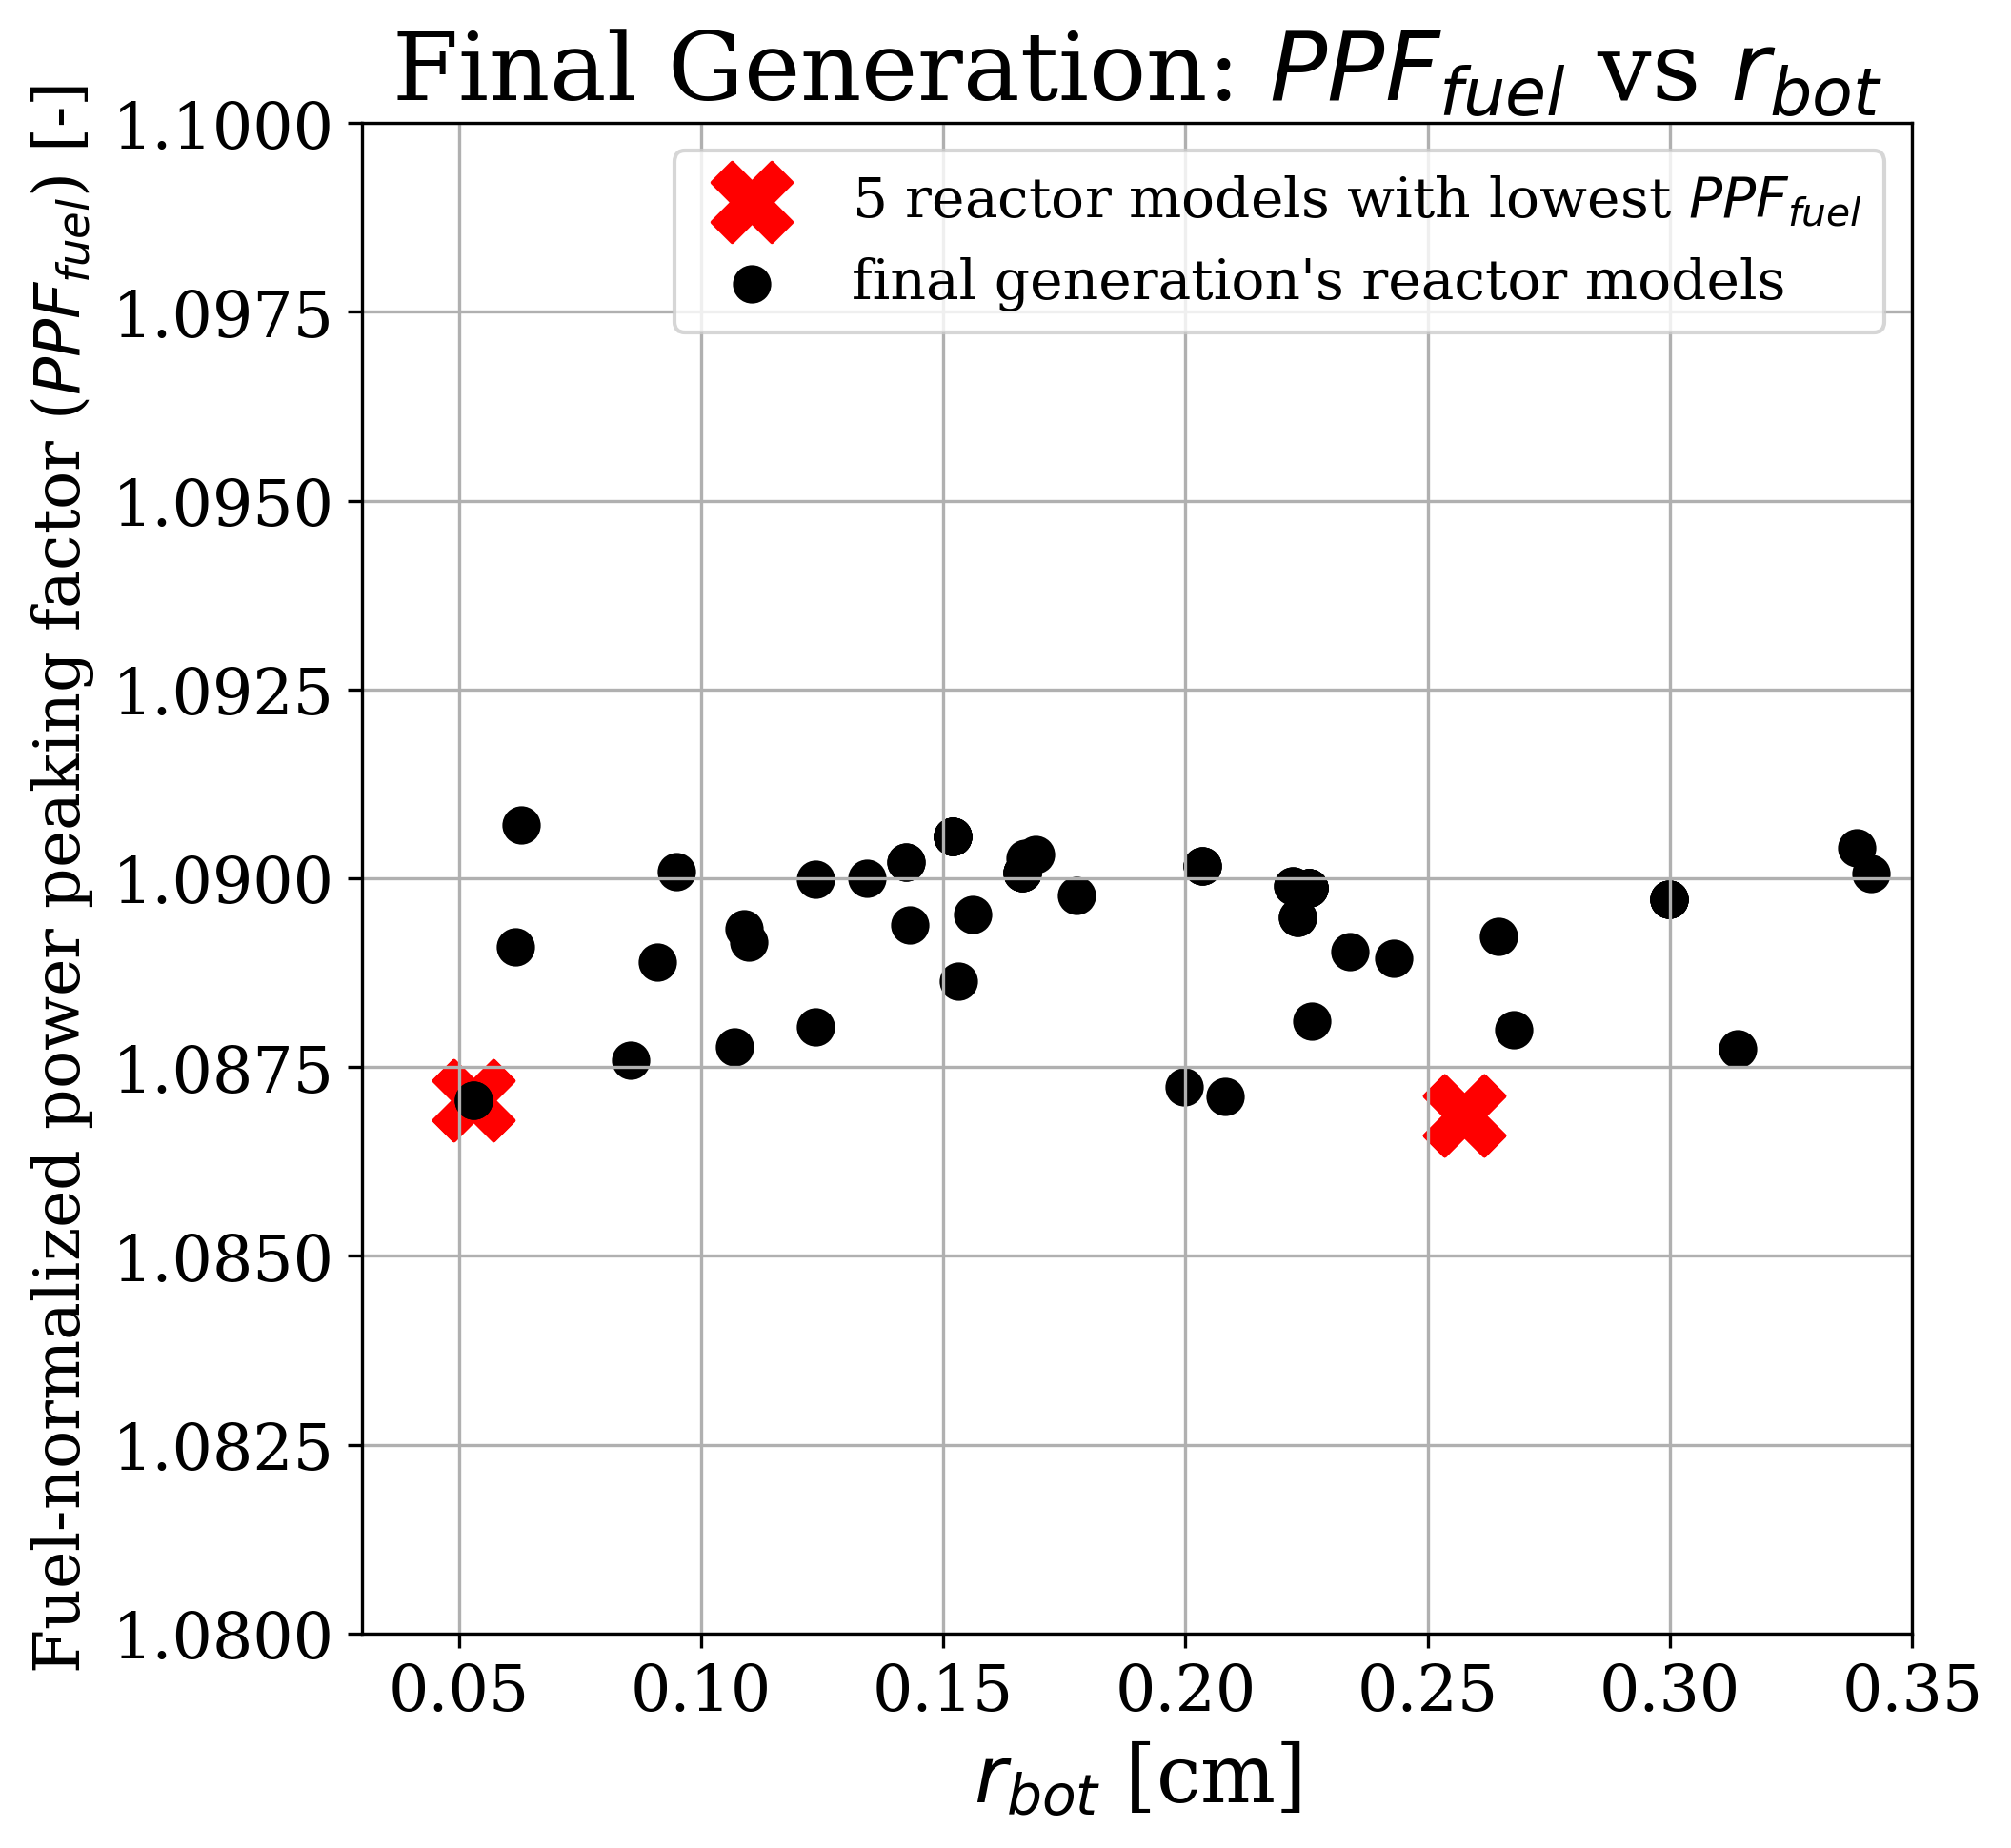
\includegraphics[width=0.49\linewidth]{slab-obj-1-ppf-final-coolant-rbot.png}
        \caption{Plot of $r_{top}$ and $r_{bot}$ against $PPF_{fuel}$. 
        Red crosses indicate the five reactor models with the lowest $PPF_{fuel}$.}
        \label{fig:slab-obj-1-ppf-final-coolant} 
    \end{subfigure}
    \caption{Simulation p-1f -- ROLLO single-objective optimization to minimize 
    fuel-normalized power peaking factor ($PPF_{fuel}$) in the slab. 
    Input parameters varied: coolant channel shape ($r_{top}, r_{bot}$). 
    $PF_{total}$ = 0.0979.}
    \label{fig:slab-obj-1-ppf-coolant}
\end{figure}
Figure \ref{fig:slab-obj-1-ppf-final-coolant} demonstrates that there is no correlation 
between $PPF_{fuel}$, and $r_{top}$ and $r_{bot}$. 

\subsection{AHTR Plank: Single-Objective Optimization Discussion}
\label{sec:plank-discussion-single}
In this section, I conduct an in-depth examination to understand and compare the 
driving factors for each individual objective. 

\subsubsection{Discussion: Minimize $PF_{total}$ Objective}
\paragraph{Simulation p-1a}
In Section \ref{sec:plank-1-obj-pf}'s simulation p-1a, I conducted a single-objective 
optimization simulation to minimize the total fuel packing fraction ($PF_{total}$) by 
varying the $PF_{total}$ and the TRISO distribution. 
In simulation p-1a, \gls{ROLLO} found that an \gls{AHTR} plank model with a
$PF_{total}$ = 0.023 and oscillating TRISO distribution most-minimized 
$PF_{total}$ while meeting the $k_{eff} \geq 1.35$ constraint 
(Figure \ref{fig:slab-obj-1-pf}). 

I ran a simulation for a constant TRISO distribution of $PF_{total}$ = 0.023 and 
compared its fission reaction rate with the oscillating TRISO distribution 
to understand why the oscillating TRISO distribution enabled a lower $PF_{total}$. 
Figure \ref{fig:triso-0.023} shows the TRISO distributions for the two compared 
simulations: Figure \ref{fig:slab-obj-1-pf}'s most-minimized $PF_{total}$ 
and the constant $PF_{total}$ = 0.023. 
\begin{figure}[htbp!]
    \centering
    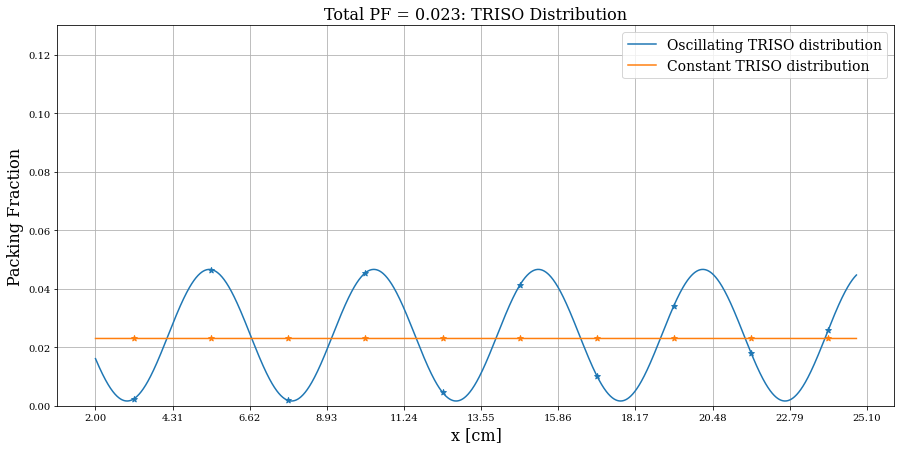
\includegraphics[width=0.9\linewidth]{triso-0.023.png} 
    \caption{Simulation p-1a's most-minimized $PF_{total}$ TRISO distribution 
    (oscillating TRISO distribution) from Figure \ref{fig:slab-obj-1-pf} and the 
    constant $PF_{total}$ = 0.023 TRISO distribution.}
    \label{fig:triso-0.023}
\end{figure}

Table \ref{tab:0.023-plank-fission-rate} compares the total fission reaction rate 
(OpenMC's \texttt{fission} tally) between the most-minimized $PF_{total}$ TRISO 
distribution and a constant $PF_{total}$ = 0.023 TRISO distribution (both shown in 
Figure \ref{fig:triso-0.023}).
\begin{table}[htbp!]
    \centering
    \onehalfspacing
    \caption{Total fission reaction rate comparison between the most-minimized 
    $PF_{total}$ TRISO distribution and a constant $PF_{total}$ = 0.023 TRISO 
    distribution. Both distributions shown in Figure \ref{fig:triso-0.023}.
    \% Fission difference is the deviation between most-minimized and flat TRISO 
    distributions' fission reaction rates.}
	\label{tab:0.023-plank-fission-rate}
    \footnotesize
    \begin{tabular}{p{1.5cm}p{3.7cm}p{3.7cm}p{2.7cm}}
    \hline
    \textbf{Energy Group} & 
    \textbf{Most-minimized $PF_{total}$ Fission \newline [reactions/src]} & 
    \textbf{Flat $PF_{total}$ Fission [reactions/src]} & 
    \textbf{$\%$ Fission Diff}\\
    \hline 
    1     & 0.001260 & 0.001234 & \Plus2.07 \\
    2     & 0.006653 & 0.006658 & \Minus0.07 \\
    3     & 0.006566 & 0.006580 & \Minus0.21 \\
    4     & 0.556897 & 0.555889 & \Plus0.18 \\
    Total & 0.542907 & 0.541924 & \Plus0.18\\
    \hline
    \end{tabular}
\end{table}
The most-minimized $PF_{total}$ TRISO distribution has $0.18\%$ higher total fission 
reaction rate than the constant $PF_{total}$ = 0.023 TRISO distribution, explaining 
why the oscillating TRISO distribution enabled a lower packing fraction 
for the same $k_{eff}$ compared to the constant TRISO distribution. 

\paragraph{Simulation p-1d}
In Section \ref{sec:plank-1-obj-pf}'s simulation p-1d, I conducted a single-objective 
optimization simulation to minimize the total fuel packing fraction ($PF_{total}$) by 
varying the $PF_{total}$ and the coolant channel shape. 
In simulation p-1a, \gls{ROLLO} found that there is no correlation 
between the $PF_{total}$ and the coolant channel shape (demonstrated in Figure 
\ref{fig:slab-obj-1-pf-final-coolant}). 

\paragraph{Summary}
The minimize $PF_{total}$ objective is driven by maximizing the total fission 
reaction rates. 
The minimize $PF_{total}$ objective has correlations with the  
$PF_{total}$ and TRISO packing fraction distribution input parameters. 
The objective has no correlation with the coolant channel shape input parameter. 

\subsubsection{Discussion: Minimize $T_{max}$ Objective}
\paragraph{Simulation p-1b}
In Section \ref{sec:plank-1-obj-temp}'s simulation p-1b, I conducted a single-objective 
optimization simulation to minimize the maximum plank temperature ($T_{max}$) by varying 
the TRISO distribution. 
In simulation p-1b, \gls{ROLLO} found that an \gls{AHTR} plank model with a mostly 
flat TRISO distribution most-minimized $T_{max}$ 
(Figure \ref{fig:slab-obj-1-temp-final}).

I found that a fully flat \gls{TRISO} distribution results in a $1.83 K$ higher $T_{max}$.
Figure \ref{fig:slab-obj-1-temp-distr} compares the Moltres-generated centerline 
temperature distribution for the plank with mostly flat (Figure 
\ref{fig:slab-obj-1-temp-final}) and flat TRISO distributions for the same 
$PF_{total}$ = 0.0979. 
\begin{figure}[htbp!]
    \centering
    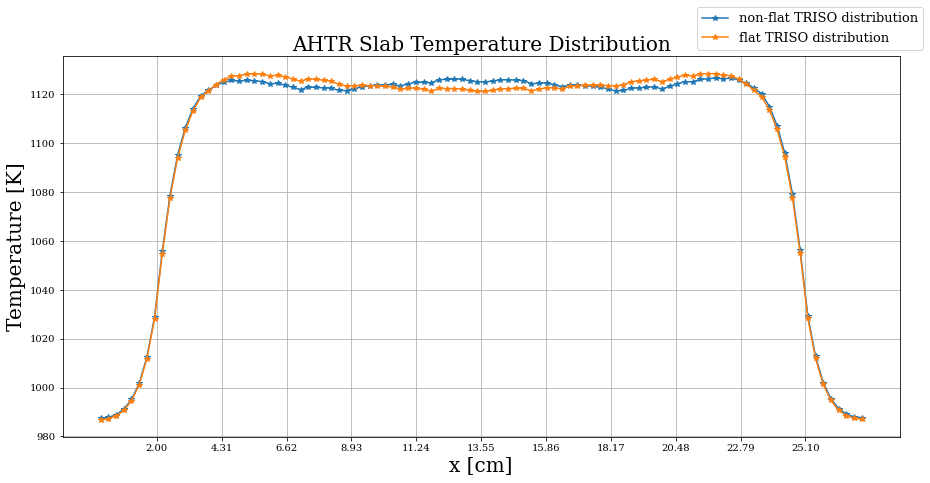
\includegraphics[width=\linewidth]{slab-obj-1-temp-distr.png}
    \caption{Comparison of Moltres-generated AHTR plank temperature distribution for 
    non-flat and flat TRISO distribution. 
    Both models have $PF_{total}$ = 0.0979.}
    \label{fig:slab-obj-1-temp-distr}
\end{figure}
The \gls{AHTR} plank with a flat \gls{TRISO} distribution has higher plank temperatures 
on the left and right sides near the moderator. 
To combat this temperature peak, ROLLO found a \gls{TRISO} distribution that 
has a slight dip near the moderator regions, resulting in a lower $T_{max}$.
However, the peak temperature discrepancy between the mostly flat and fully flat 
TRISO distributions is very small. 
Thus, the minimize $T_{max}$ objective mainly flattens the TRISO distribution.

\paragraph{Simulation p-1e}
In Section \ref{sec:plank-1-obj-temp}'s simulation p-1e, I conducted a single-objective 
optimization simulation to minimize the maximum plank temperature ($T_{max}$) by varying 
the coolant channel shape. 
In simulation p-1e, \gls{ROLLO} found that there is a negative linear correlation 
between the plank's $T_{max}$, and $r_{bot}$ and $r_{top}$, shown in 
Figure \ref{fig:slab-obj-1-temp-final-coolant}. 
Comparison of simulation p-1b and p-1e's results in 
Figures \ref{fig:slab-obj-1-temp-evol} and \ref{fig:slab-obj-1-temp-evol-coolant} show 
that the average $T_{max}$ due to \gls{TRISO} variation decreased by 60K over 
10 generations, while average $T_{max}$ due to the coolant channel shape variation 
only decreased by 15K over 10 generations. 
This demonstrates that during the genetic algorithm optimization process, 
variations in the coolant channel shape only minimize $T_{max}$ by 15K, while
variations in the TRISO distribution minimizes $T_{max}$ by 60K. 
The TRISO distribution variations have a higher impact on the $T_{max}$ value compared 
to coolant channel variation, highlighting to reactor designers that for minimizing 
the $T_{max}$ objective, they should pay more attention to the fuel density 
distribution in the \gls{AHTR} design compared to coolant channel shape.  

\paragraph{Summary}
The minimize $T_{max}$ objective flattens the TRISO distribution and maximizes the 
coolant channel shape's $r_{bot}$ and $r_{top}$ to achieve the objective. 
The minimize $T_{max}$ objective has correlations with all the input parameters: 
$PF_{total}$, TRISO packing fraction distribution, and coolant channel shape. 
The results from simulation p-1b and p-1e suggest that the minimize $T_{max}$ objective 
is more influenced by the TRISO distribution than the coolant channel shape. 

\subsubsection{Discussion: Minimize $PPF_{fuel}$ Objective}
I conduct an equation analysis to determine the \gls{AHTR} plank properties 
that influence the $PPF_{fuel}$ objective. 
I then demonstrate the derived relationship in simulation p-1c results.

\paragraph{Equation Analysis}
Equation \ref{eq:reaction-rate-fission} shows the relationship between fission reaction 
rate, flux, and material properties: 
\begin{align}
\label{eq:reaction-rate-fission}
    RR_f &= \Phi \times \sigma_f \times N \\
\intertext{where}
    RR_f &= \mbox{fission reaction rate } [reactions \cdot cm^{-3} \cdot s^{-1}] \nonumber \\
    \Phi &= \mbox{neutron flux } [neutrons \cdot cm^{-2} \cdot s^{-1}] \nonumber \\
    \sigma_f &= \mbox{microscopic cross section } [cm^2] \nonumber \\
    N &= \mbox{atomic number density } [atoms \cdot cm^{-3}] \nonumber 
\end{align}

Since microscopic cross section is constant for the same fuel material, I rearrange 
Equation \ref{eq:reaction-rate-fission} into Equation \ref{eq:reaction-rate-fission-prop}: 
\begin{align}
    \label{eq:reaction-rate-fission-prop}
    \Phi \propto \frac{RR_f}{N}
\end{align}
In Section \ref{sec:ahtr_slab_output}, I defined the fuel-normalized power peaking 
factor ($PPF_{fuel}$) as: 
\begin{align}
    PPF_{fuel} &= \frac{max(\frac{fqr_j}{PF_j})}{ave(\frac{fqr_j}{PF_j})}
\intertext{where}
PPF_{fuel} &= \mbox{fuel-normalized power peaking factor} \nonumber \\
j &= \mbox{discretized fuel area j} \nonumber \\
fqr_j &= \mbox{fission-q-recoverable at position j (OpenMC tally)} \nonumber \\
PF_j &= \mbox{fuel packing fraction at position j} \nonumber
\end{align}
The fission reaction rate ($RR_f$) is proportional to fission energy production rate 
($fqr$). 
The atomic number density (N) is proportional to the fuel packing fraction ($PF$). 
Thus, I can rearrange Equation \ref{eq:reaction-rate-fission-prop} into 
Equation \ref{eq:flux-prop-fqr}:
\begin{align}
    \label{eq:flux-prop-fqr}
    \Phi_j \propto \frac{fqr_j}{PF_j}
\end{align}
Finally, I can further rearrange Equation \ref{eq:flux-prop-fqr} into 
Equation \ref{eq:flux-prop-ppf}:
\begin{align}
    \label{eq:flux-prop-ppf}
    \frac{max(\Phi_j)}{ave(\Phi_j)} &\propto \frac{max(\frac{fqr_j}{PF_j})}{ave(\frac{fqr_j}{PF_j})} \nonumber \\
    \frac{max(\Phi_j)}{ave(\Phi_j)} &\propto PPF_{fuel}
\end{align}

Therefore, from Equation \ref{eq:flux-prop-ppf}, a flatter flux (smaller 
$\frac{max(\Phi_j)}{ave(\Phi_j)}$ value) will result in a smaller $PPF_{fuel}$. 
Specifically, flatter energy group 4 thermal flux results in a smaller $PPF_{fuel}$
(see Table \ref{tab:fission-flux}). 
Table \ref{tab:fission-flux} shows the percentage contributions of fission reactions from 
each energy group from the constant $PF_{total}$ = 0.0979 TRISO distribution 
shown in Figure \ref{fig:triso-0.0979}. 
\begin{table}[htbp!]
    \centering
    \onehalfspacing
    \caption{Percentage of fission reactions from each energy group for \gls{AHTR} plank model.}
	\label{tab:fission-flux}
    \footnotesize
    \begin{tabular}{llc}
    \hline 
    \textbf{Energy Group} & \textbf{Energy Bounds [MeV]} & \textbf{\% of Total Fission \newline Reactions} \\
    \hline
    1 & $9.1188\times 10^{-3} < E < 2.0000\times 10^1$ & 0.85 \\ 
    2 & $2.9023\times 10^{-5} < E < 9.1188\times 10^{-3}$ & 4.85 \\
    3 & $1.8554\times 10^{-6} < E < 2.9023\times 10^{-5}$ & 4.14 \\
    4 & $1.0000\times 10^{-12} < E < 1.8554\times 10^{-6}$ & 90.14 \\
    \hline
    \end{tabular}
\end{table}
Most fission reactions are occurring in energy group 4. 

In the following section, I demonstrate Equation \ref{eq:flux-prop-ppf}'s relationship 
in simulation p-1c results. 

\paragraph{Simulation p-1c}
In Section \ref{sec:plank-1-obj-ppf}'s simulation p-1c, I conducted a single-objective 
optimization simulation to minimize the fuel-normalized power peaking factor ($PPF_{fuel}$) 
by varying TRISO distribution. 
In simulation p-1c, \gls{ROLLO} found that for $PF_{total}$ = 0.0979, an \gls{AHTR} 
plank model with the TRISO distribution that peaks near the edges of the fuel region of 
the plank and a minimum point in plank's center with a variation of $\sim0.07$, 
most-minimized $PPF_{fuel}$ (Figure \ref{fig:slab-obj-1-ppf}). 

I ran a simulation for constant $PF_{total}$ = 0.0979 and compared its 
flux to simulation p-1c's most-minimized $PPF_{fuel}$ TRISO distribution to understand 
why the latter enabled a lower $PPF_{fuel}$. 
Figure \ref{fig:triso-0.0979} shows the TRISO distributions and the $PPF_{fuel}$ 
values for the two compared simulations: simulation p-1c's (Figure 
\ref{fig:slab-obj-1-ppf}) most-minimized $PPF_{fuel}$ TRISO distribution and 
the constant $PF_{total}$ = 0.0979 TRISO distribution. 
\begin{figure}[htbp!]
    \centering
    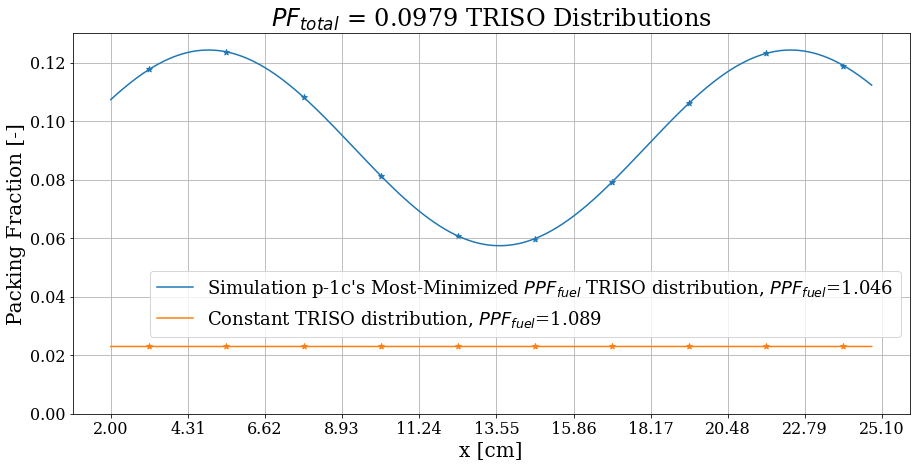
\includegraphics[width=0.9\linewidth]{triso-0.0979.png} 
    \caption{Simulation p-1c's most-minimized $PPF_{fuel}$ TRISO distribution 
    from Figure \ref{fig:slab-obj-1-ppf} and the constant $PF_{total}$ = 0.0979 
    TRISO distribution.}
    \label{fig:triso-0.0979}
\end{figure}

Figure \ref{fig:flux-comparison-0.0979-plank} compares the flux distributions between 
the most-minimized $PPF_{fuel}$ TRISO distribution and the constant $PF_{total}$ = 0.0979 
TRISO distribution (both shown in Figure \ref{fig:triso-0.0979}).
\begin{figure}[htbp!]
    \centering
    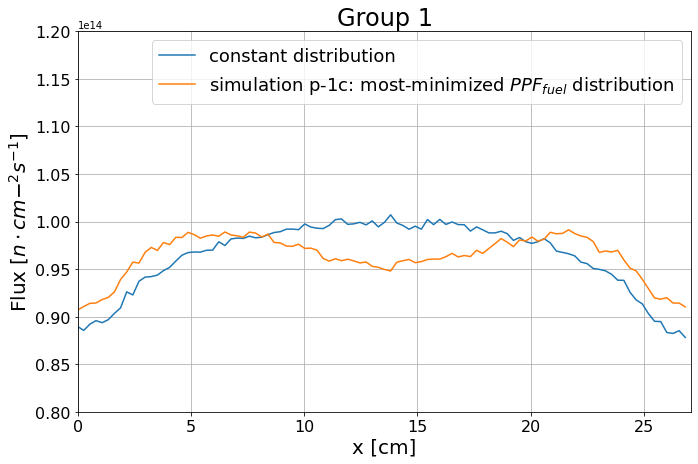
\includegraphics[width=0.48\linewidth]{flux-comparison-0.0979-plank_grp1.png} 
    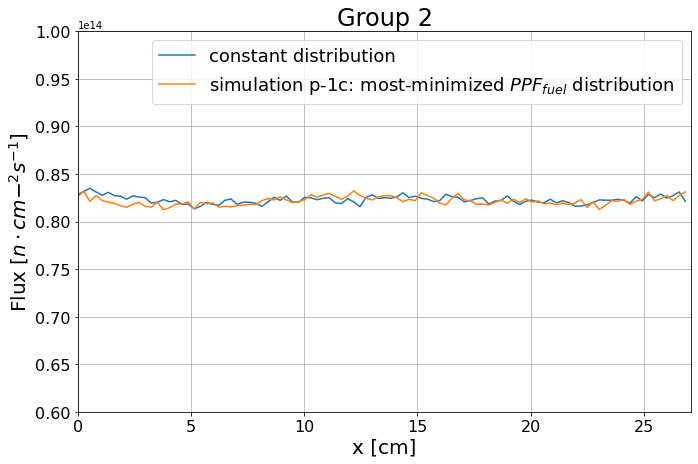
\includegraphics[width=0.48\linewidth]{flux-comparison-0.0979-plank_grp2.png} 
    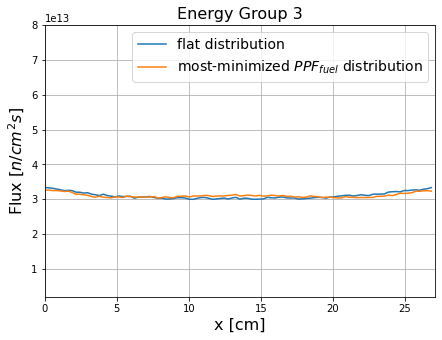
\includegraphics[width=0.48\linewidth]{flux-comparison-0.0979-plank_grp3.png} 
    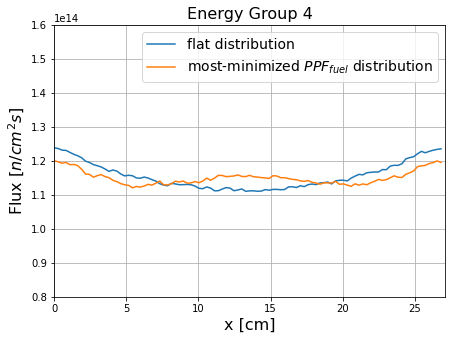
\includegraphics[width=0.48\linewidth]{flux-comparison-0.0979-plank_grp4.png} 
    \caption{Flux comparison between Figure \ref{fig:slab-obj-1-ppf-final}'s TRISO 
    distribution that most-minimized $PPF_{fuel}$ and a constant $PF_{total}$ = 0.0979 
    TRISO distribution. 
    \gls{AHTR} plank's centerline neutron flux distribution in 4 groups at 948K. 
    The centerline is the white line in Figure \ref{fig:ahtr-plank-verification}.
    Energy Group 1: E $> 9.1188 \times 10^{-3}$ MeV;
    Energy Group 2: $2.9023 \times 10^{-5} < E < 9.1188 \times 10^{-3}$ MeV;
    Energy Group 3:  $1.8556 \times 10^{-5} < E < 2.9023 \times 10^{-5}$ MeV;
    Energy Group 4:  $1.0 \times 10^{-12} < E < 1.8554 \times 10^{-6}$ MeV.}
    \label{fig:flux-comparison-0.0979-plank}
\end{figure}

In Figure \ref{fig:flux-comparison-0.0979-plank}, the constant TRISO distribution's 
Group 4 flux dips in the center of the plank due to spatial self-shielding effects. 
In the constant TRISO distribution's Group 1 flux, there is a peak in fast neutrons
born in the plank's center, the fast neutrons are moderated in the graphite matrix 
and graphite structure (Figure \ref{fig:straightened_plank}). 
The self-shielding neutrons are more likely absorbed at the fuel regions at the 
plank's sides, near the pure graphite structure moderating regions. 
The outer sides of the plank absorb these neutrons and geometrically shield the 
plank's center from neutron flux, leading to a relatively lower group 4 thermal 
flux in the plank's center for the constant TRISO distribution. 

Table \ref{tab:flux-comparison-0.0979-plank} quantifies the flux comparison 
from Figure \ref{fig:flux-comparison-0.0979-plank} between simulation p-1c's 
most-minimized $PPF_{fuel}$ TRISO distribution and the constant 
$PF_{total}$ = 0.0979 TRISO distribution (both shown in Figure \ref{fig:triso-0.0979}).
\begin{table}[htbp!]
    \centering
    \onehalfspacing
    \caption{Flux value comparison between Figure \ref{fig:slab-obj-1-ppf-final}'s TRISO 
    distribution that most-minimized $PPF_{fuel}$ and a constant $PF_{total}$ = 0.0979 
    TRISO distribution. 
    Energy Group 1: E $> 9.1188 \times 10^{-3}$ MeV;
    Energy Group 2: $2.9023 \times 10^{-5} < E < 9.1188 \times 10^{-3}$ MeV;
    Energy Group 3:  $1.8556 \times 10^{-5} < E < 2.9023 \times 10^{-5}$ MeV;
    Energy Group 4:  $1.0 \times 10^{-12} < E < 1.8554 \times 10^{-6}$ MeV.}
	\label{tab:flux-comparison-0.0979-plank}
    \footnotesize
    \begin{tabular}{lp{4.2cm}p{3.3cm}p{4cm}}
    \hline
    \textbf{Energy Group} &
    \textbf{$max(\phi)/min(\phi)$ \newline Most-minimized $PPF_{fuel}$ \newline TRISO Distribution} & 
    \textbf{$max(\phi)/min(\phi)$ \newline Constant TRISO \newline Distribution} & 
    \textbf{$\%$ Diff}\\
    \hline 
    1 & 1.093 & 1.147 & \Minus4.68 \\
    2 & 1.024 & 1.027 & \Minus0.22\\
    3 & 1.077 & 1.114 & \Minus3.32 \\
    4 & 1.071 & 1.115 & \Minus3.96 \\
    \hline
    \end{tabular}
\end{table}

In energy group 4, the most-minimized $PPF_{fuel}$ flux distribution is $3.96\%$ flatter 
than the constant $PF_{total}$ = 0.0979 flux distribution, resulting in a lower 
$PPF_{fuel}$ (as shown by Equation \ref{eq:flux-prop-ppf}). 
% TODO: major takeaway 

\paragraph{Simulation p-1f}
In Section \ref{sec:plank-1-obj-ppf}'s simulation p-1f, I conducted a single-objective 
optimization simulation to minimize the fuel-normalized power peaking factor ($PPF_{fuel}$) 
by varying the coolant channel shape.
Comparison of simulation p-1c and p-1f's results in Figures 
\ref{fig:slab-obj-1-ppf-evol-coolant} and \ref{fig:slab-obj-1-ppf-evol}
show that the coolant channel shape variation barely has an impact on $PPF_{fuel}$ as 
\gls{TRISO} distribution variation: the average $PPF_{fuel}$ due to \gls{TRISO} 
variation decreased by 0.1 over 10 generations, while average $PPF_{fuel}$ due to 
coolant channel shape variation only decreased negligibly over 10 generations. 
Figure \ref{fig:slab-obj-1-ppf-final-coolant} reiterates that there is no correlation 
between total radius and $PPF_{fuel}$. 

\paragraph{Summary}
The minimize $PPF_{fuel}$ objective is driven by flattening thermal (Group 4) flux 
distribution. 
The minimize $PPF_{fuel}$ objective has correlations with the following input parameters: 
$PF_{total}$ and TRISO packing fraction distribution. 
The objective has no correlation with the coolant channel shape input parameter.

\subsection{AHTR Plank: Single-Objective Optimization Major Takeaways}


\section{AHTR Plank: Two-Objective Optimization Results}
\label{sec:plank-two-obj}
This section reports the \gls{AHTR} plank's \gls{ROLLO} two-objective 
optimization results. 
The previous section's single-objective optimization results inform the multi-objective 
optimization simulations in this section and Section \ref{sec:plank-three-obj}.
Since the variations in coolant channel shape only impact one objective, 
the minimize plank's maximum temperature ($T_{max}$), I do not conduct two-objective 
optimization for coolant channel shape variations.  
Table \ref{tab:slab-obj-breakdown} summarized the two-objective simulations in this 
section: p-2a, p-2b, and p-2c.

As previously described in Section \ref{sec:opt}, multi-objective optimization returns 
multiple optimal solutions that meet each objective to varying degrees; this set of 
solutions is the Pareto front \cite{deb_multi-objective_2001}. 
For each solution in the Pareto front, none of the objective functions can be 
improved without degrading another objective.
An ideal optimization method for a multi-objective problem, like reactor design 
optimization, should find widely spread solutions in the obtained Pareto front 
\cite{deb_multi-objective_2001}. 
Thus, I report the optimal reactor models on the Pareto front for the multi-objective 
optimization problems in this section and Section \ref{sec:plank-three-obj}. 

To ensure that the multi-objective optimization problems are converged, I report the 
hypervolume values for each generation. 
As previously described in Section \ref{sec:binhandkorn}, the hypervolume indicator 
quantifies the Pareto front's goodness (bigger = better).
I use a different reference point for each optimization problem. 
If a multi-objective optimization problem's hypervolume converges earlier than the 
five generations I intended to run (determined in Section 
\ref{sec:multi-obj-hyperparameters}), I stop the simulation at that generation. 
However, if the multi-objective optimization problem's hypervolume does not converge by 
generation 5, I run the problem for a few more generations till satisfactory convergence.

\subsection{p-2a: Minimize $PF_{total}$ and $T_{max}$}
\label{sec:p-2a}
This section reports results from the two-objective optimization simulation p-2a; the 
objectives minimized are total fuel packing fraction ($PF_{total}$) and maximum plank
temperature ($T_{max}$).  
Table \ref{tab:simulationp2a} shows simulation p-2a's optimization problem parameters.
\begin{table}[htbp!]
    \centering
    \onehalfspacing
    \caption{Simulation p-2a optimization problem parameters.}
	\label{tab:simulationp2a}
    \footnotesize
    \begin{tabular}{l|p{4cm}}
    \hline 
    \multicolumn{2}{c}{\textbf{Two Objectives: Simulation p-2a}} \\
    \hline 
    \textbf{Objectives} & Minimize $PF_{total}$ \\
    & Minimize $T_{max}$ \\
    \hline 
    \textbf{Input parameter variations} & $0.02 \leq PF_{total} \leq 0.04$ \\
    & $\rho_{TRISO}(\vec{r})$: $0<a<2$ \\
    & $\rho_{TRISO}(\vec{r})$: $0<b<\frac{\pi}{2}$ \\
    & $\rho_{TRISO}(\vec{r})$: $0<c<2\pi$ \\
    \hline
    \textbf{Constraints} & $k_{eff} \geq 1.35$\\ 
    \hline 
    \textbf{Genetic algorithm parameters} & Population size: 128 \\
    & Generations: 2 \\
    \hline
    \end{tabular}
\end{table}

Table \ref{tab:p2a-hypervolume} shows each generation's hypervolume values, 
confirming that simulation p-2a converges by generation 2. 
\begin{table}[htbp!]
    \centering
    \onehalfspacing
    \caption{Simulation p-2a hypervolume values at each generation.}
	\label{tab:p2a-hypervolume}
    \footnotesize
    \begin{tabular}{ll}
    \hline 
    \multicolumn{2}{c}{\textbf{Two Objectives: Simulation p-2a}} \\
    \multicolumn{2}{c}{Reference point: (0.1, 1350)} \\
    \hline 
    \textbf{Generation} & \textbf{Hypervolume [-]} \\
    \hline
    1 & 17.659 \\
    2 & 17.659 \\
    \hline
    \end{tabular}
\end{table}

Figure \ref{fig:slab-obj-2-pftemp-pareto} shows a plot of the final generation's 
$PF_{total}$ against $T_{max}$; crosses mark the reactor models that 
fall on the Pareto front.
Figure \ref{fig:slab-obj-2-pftemp-pareto-distr} shows the six TRISO distributions in 
the final generation that fall on the Pareto front.
Figures \ref{fig:slab-obj-2-pftemp-min-pf} and \ref{fig:slab-obj-2-pftemp-min-temp} 
illustrate the \gls{AHTR} plank models with the most-minimized $PF_{total}$ and 
$T_{max}$, respectively.  
\begin{figure}[htbp!]
    \centering
    \begin{subfigure}{\textwidth}
        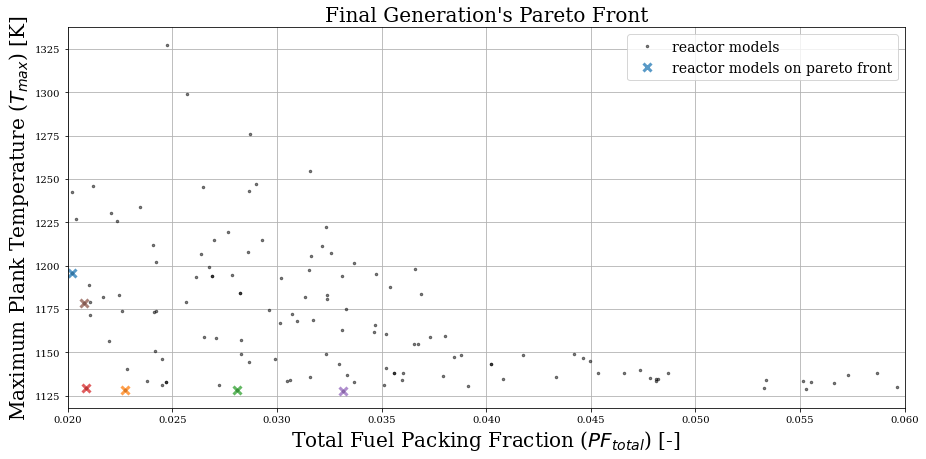
\includegraphics[width=\linewidth]{slab-obj-2-pftemp-pareto.png}
        \caption{Plot of final generation's reactor models' $PF_{total}$ against 
        $T_{max}$. Crosses indicate the reactor models on the Pareto front and the 
        colors correspond to TRISO distributions in Figure 
        \ref{fig:slab-obj-2-pftemp-pareto-distr} .}
        \label{fig:slab-obj-2-pftemp-pareto} 
    \end{subfigure}
    \begin{subfigure}{\textwidth}
        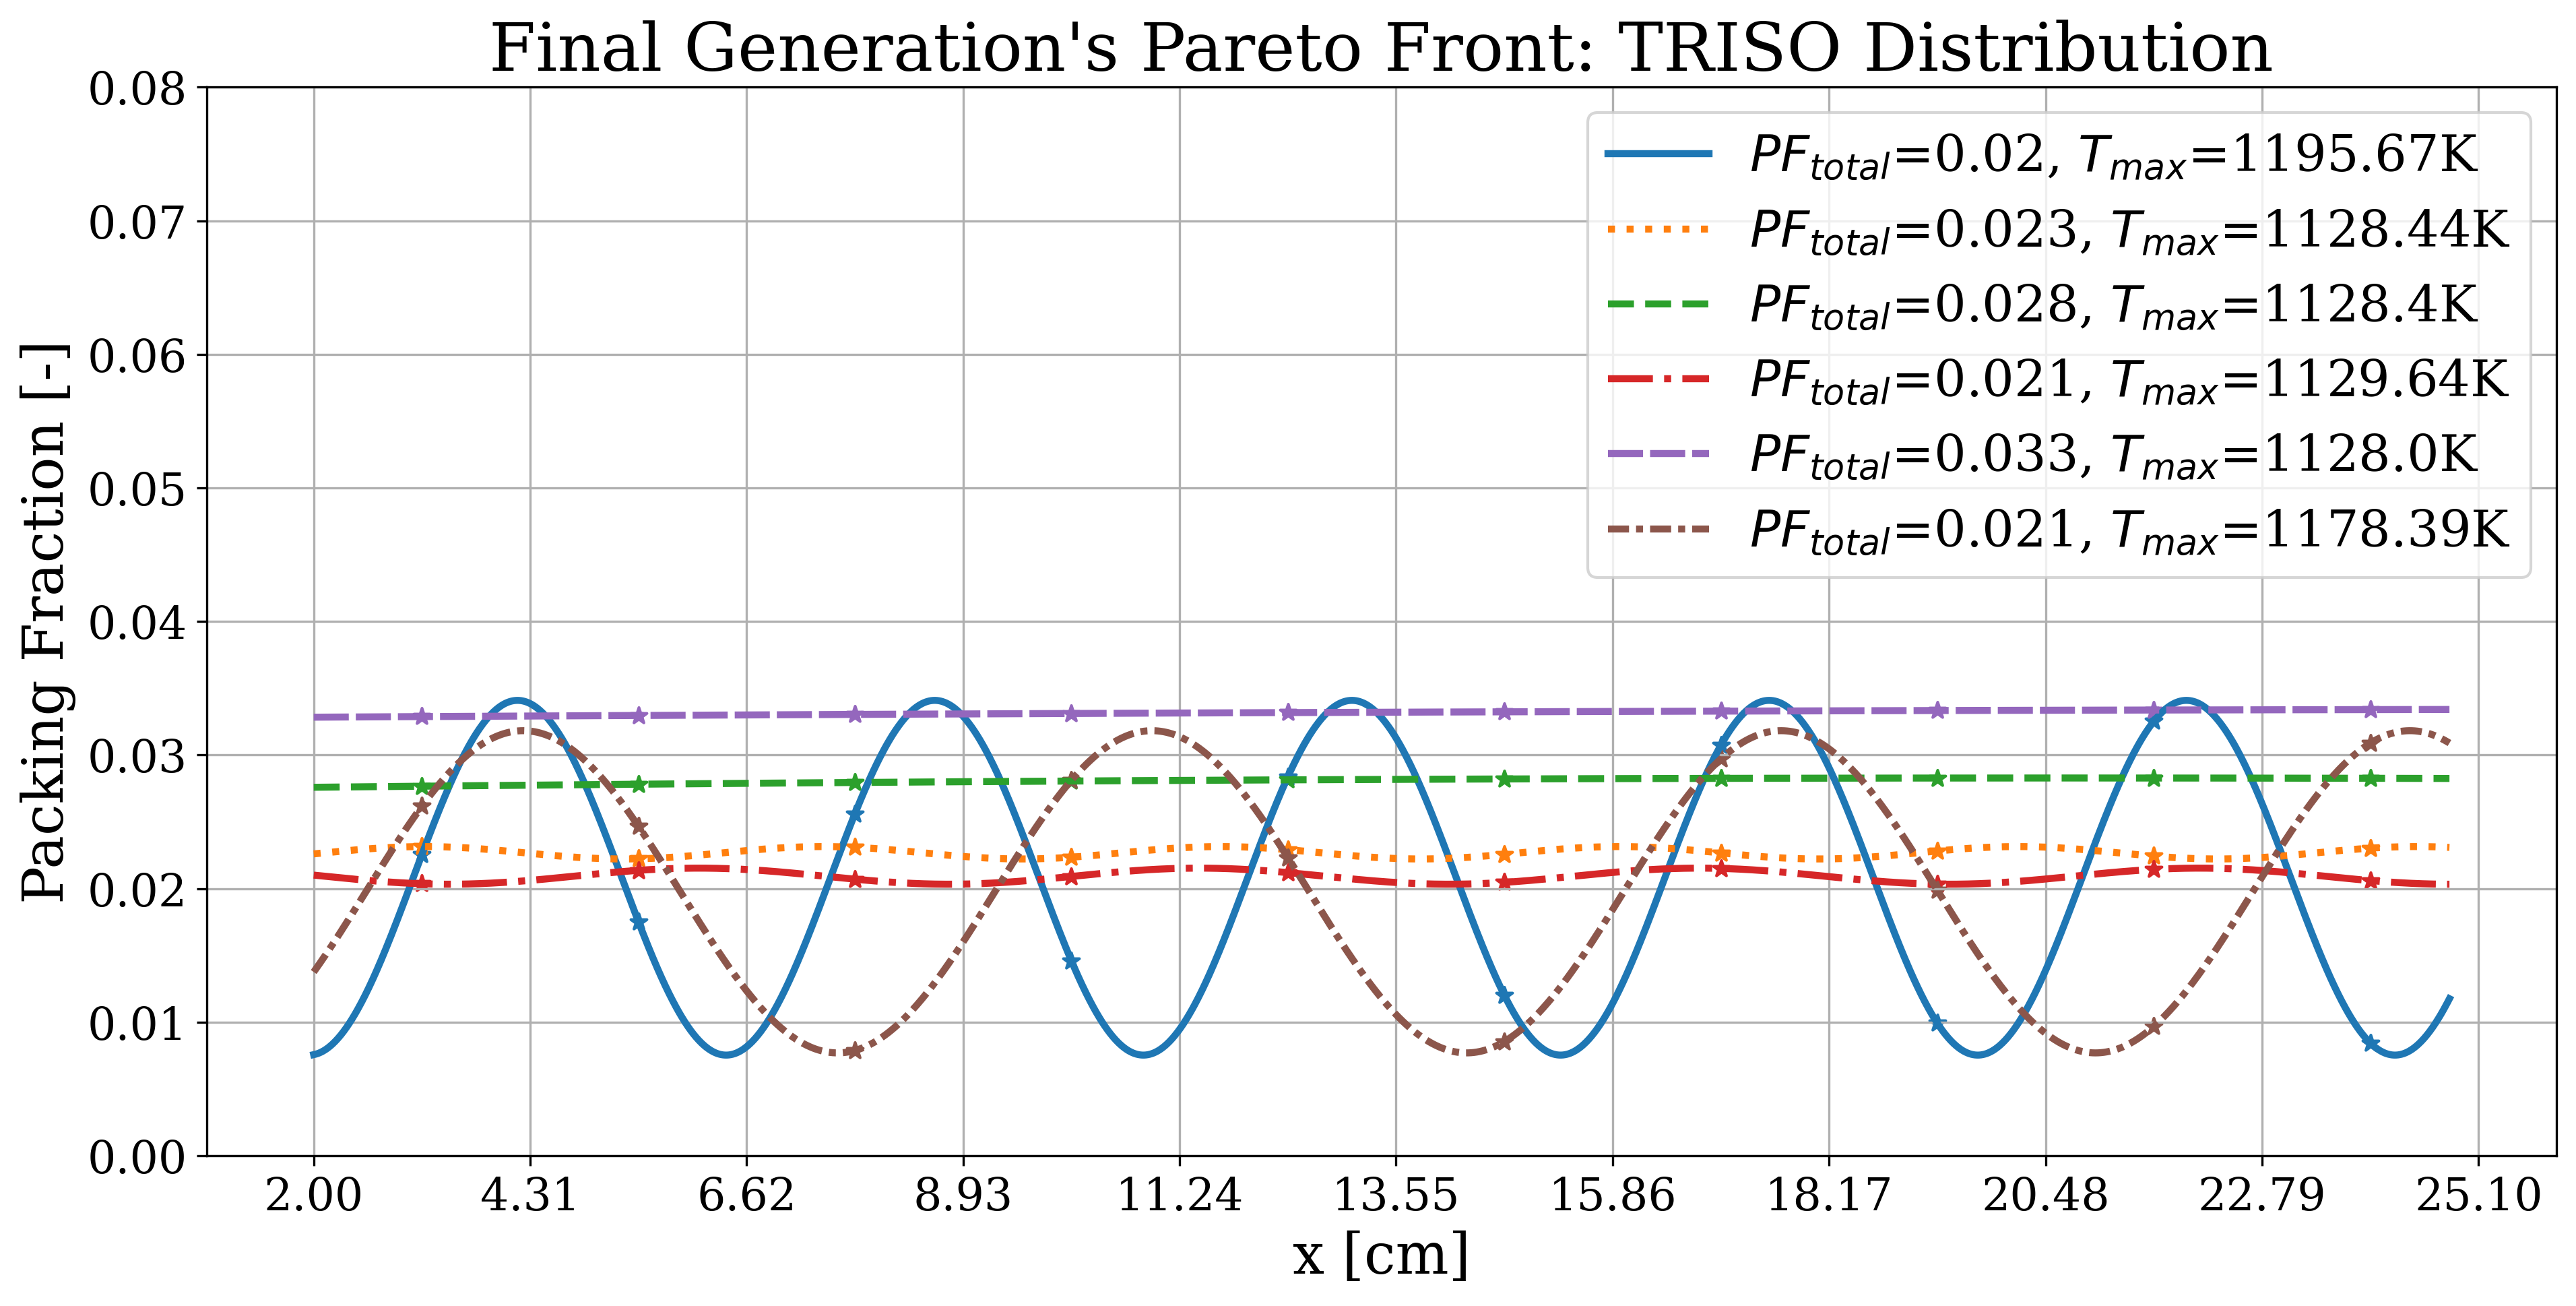
\includegraphics[width=\linewidth]{slab-obj-2-pftemp-pareto-distr.png}
        \caption{TRISO packing fraction distribution for the six reactor models on the 
        Pareto front.}
        \label{fig:slab-obj-2-pftemp-pareto-distr} 
    \end{subfigure}
    \caption{Simulation p-2a -- ROLLO two-objective optimization to minimize the total 
    fuel packing fraction ($PF_{total}$) and maximum plank temperature ($T_{max}$). 
    Input parameters varied: total fuel packing fraction ($PF_{total}$), 
    \gls{TRISO} distribution ($\rho_{TRISO}(\vec{r})$).}
    \label{fig:slab-obj-2-pftemp}
\end{figure}
\begin{figure}[htbp!]
    \ContinuedFloat
    \begin{subfigure}{\textwidth}
        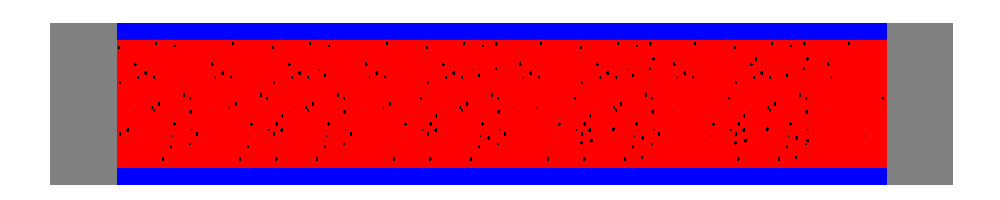
\includegraphics[width=\linewidth]{slab-obj-2-pftemp-min-pf.png}
        \caption{\gls{AHTR} plank model with the most-minimized $PF_{total}$
        (corresponds to the blue solid distribution in Figure 
        \ref{fig:slab-obj-2-pftemp-pareto-distr}). $PF_{total} = 0.02$, 
        $T_{max} = 1195.67K$.}
        \label{fig:slab-obj-2-pftemp-min-pf} 
    \end{subfigure}
    \begin{subfigure}{\textwidth}
        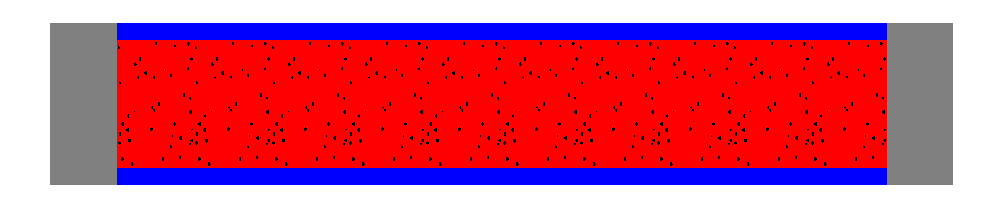
\includegraphics[width=\linewidth]{slab-obj-2-pftemp-min-temp.png}
        \caption{\gls{AHTR} plank model with the most-minimized $T_{max}$
        (corresponds to the purple densely dashed distribution in Figure 
        \ref{fig:slab-obj-2-pftemp-pareto-distr}). $PF_{total} = 0.033$, 
        $T_{max} = 1128.0K$.}
        \label{fig:slab-obj-2-pftemp-min-temp} 
    \end{subfigure}
    \caption{(contd.) Simulation p-2a -- ROLLO two-objective optimization to minimize 
    the total packing fraction ($PF_{total}$) and maximum plank temperature ($T_{max}$). 
    Input parameters varied: total fuel packing fraction ($PF_{total}$), 
    \gls{TRISO} packing fraction distribution ($\rho_{TRISO}(\vec{r})$).}
\end{figure}

In Figure \ref{fig:slab-obj-2-pftemp-pareto}, \gls{ROLLO} finds six widely spread 
reactor model solutions on simulation p-2a's Pareto front. 
These \gls{TRISO} distributions on the Pareto front that minimize both $PF_{total}$ and 
$T_{max}$ vary between the two extreme cases: 
most-minimized $PF_{total}$ and most-minimized $T_{max}$. 
In Figure \ref{fig:slab-obj-2-pftemp-pareto-distr}, the plank model with the
most-minimized $PF_{total}$ and the highest $T_{max}$ (the blue solid distribution) 
has an oscillating TRISO distribution (also illustrated in Figure 
\ref{fig:slab-obj-2-pftemp-min-pf}).
In Figure \ref{fig:slab-obj-2-pftemp-pareto-distr}, the plank model with the 
most-minimized $T_{max}$ and highest $PF_{total}$ (the purple densely dashed distribution)
has an almost constant TRISO distribution of $PF_{total}=0.032$ across the plank (also 
illustrated in Figure \ref{fig:slab-obj-2-pftemp-min-temp}). 
Section \ref{sec:plank-discussion-multi} discusses and explains simulation p-2a's results.

\subsection{p-2b: Minimize $PF_{total}$ and $PPF_{fuel}$}
\label{sec:p-2b}
This section reports results from the two-objective optimization simulation p-2b; the 
objectives minimized are total fuel packing fraction ($PF_{total}$) and fuel-normalized 
power peaking factor ($PPF_{fuel}$).  
Table \ref{tab:simulationp2b} shows simulation p-2b's optimization problem parameters. 
\begin{table}[htbp!]
    \centering
    \onehalfspacing
    \caption{Simulation p-2b optimization problem parameters.}
	\label{tab:simulationp2b}
    \footnotesize
    \begin{tabular}{l|p{4cm}}
    \hline 
    \multicolumn{2}{c}{\textbf{Two Objectives: Simulation p-2b}} \\
    \hline 
    \textbf{Objectives} & Minimize $PF_{total}$ \\
    & Minimize $PPF_{fuel}$ \\
    \hline 
    \textbf{Input parameter variations} & $0.02 \leq PF_{total} \leq 0.04$ \\
    & $\rho_{TRISO}(\vec{r})$: $0<a<2$ \\
    & $\rho_{TRISO}(\vec{r})$: $0<b<\frac{\pi}{2}$ \\
    & $\rho_{TRISO}(\vec{r})$: $0<c<2\pi$ \\
    \hline
    \textbf{Constraints} & $k_{eff} \geq 1.35$\\ 
    \hline 
    \textbf{Genetic algorithm parameters} & Population size: 128 \\
    & Generations: 3 \\
    \hline
    \end{tabular}
\end{table}

Table \ref{tab:p2b-hypervolume} shows each generation's hypervolume value, 
confirming that simulation p-2b converges by generation 3. 
\begin{table}[htbp!]
    \centering
    \onehalfspacing
    \caption{Simulation p-2b hypervolume values at each generation.}
	\label{tab:p2b-hypervolume}
    \footnotesize
    \begin{tabular}{ll}
    \hline 
    \multicolumn{2}{c}{\textbf{Two Objectives: Simulation p-2b}} \\
    \multicolumn{2}{c}{Reference point: (0.1, 1.5)} \\
    \hline 
    \textbf{Generation} & \textbf{Hypervolume [-]} \\
    \hline
    1 & 0.03607 \\
    2 & 0.03619 \\
    3 & 0.03625 \\
    \hline
    \end{tabular}
\end{table}

Figure \ref{fig:slab-obj-2-pfppf-pareto} shows a plot of the final generation's 
$PF_{total}$ against $PPF_{fuel}$; crosses mark the reactor models that fall on 
the Pareto front.
Figure \ref{fig:slab-obj-2-pfppf-pareto-distr} shows the four TRISO packing fraction 
distributions in the final generation that fall on the Pareto front. 
Figures \ref{fig:slab-obj-2-pfppf-min-pf} and \ref{fig:slab-obj-2-pfppf-min-ppf} 
illustrate the \gls{AHTR} plank models with the most-minimized $PF_{total}$ and 
$PPF_{fuel}$, respectively. 
\begin{figure}[htbp!]
    \centering
    \begin{subfigure}{\textwidth}
        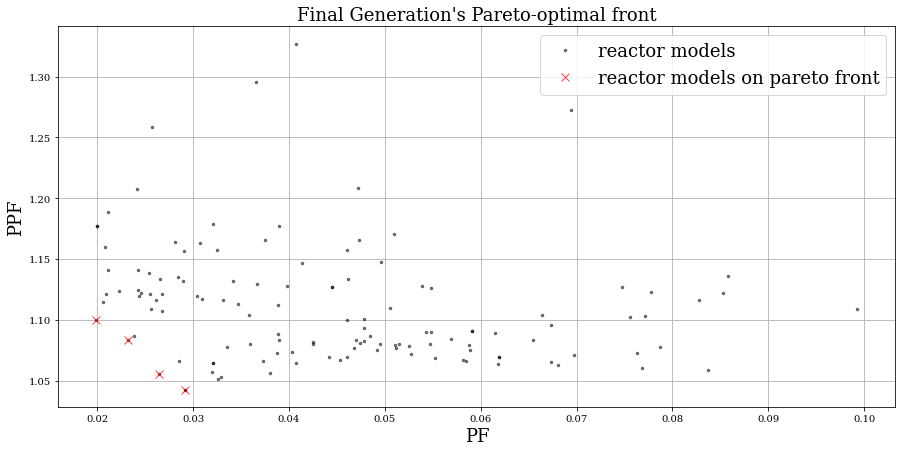
\includegraphics[width=\linewidth]{slab-obj-2-pfppf-pareto.png}
        \caption{Plot of final generation's reactor models' $PF_{total}$ against 
        $PPF_{fuel}$. 
        Crosses indicate the reactor models on the Pareto front. Cross colors correspond  
        to TRISO distributions in the plot below.}
        \label{fig:slab-obj-2-pfppf-pareto} 
    \end{subfigure}
    \begin{subfigure}{\textwidth}
        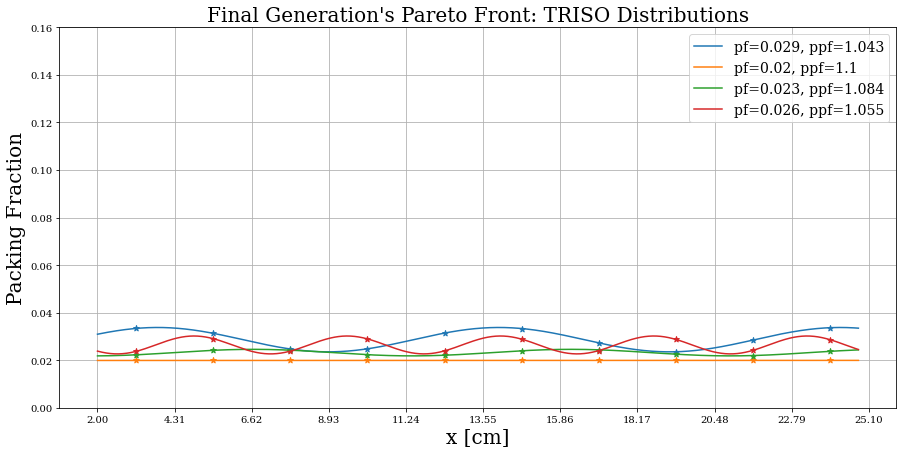
\includegraphics[width=\linewidth]{slab-obj-2-pfppf-pareto-distr.png}
        \caption{TRISO distribution for the four reactor models on the Pareto front.}
        \label{fig:slab-obj-2-pfppf-pareto-distr} 
    \end{subfigure}
    \caption{Simulation p-2b -- ROLLO two-objective optimization to minimize total fuel 
    packing fraction ($PF_{total}$) and normalized power peaking factor ($PPF_{fuel}$) 
    in the plank. 
    Input parameters varied: TRISO packing fraction distribution 
    ($\rho_{TRISO}(\vec{r})$).}
    \label{fig:slab-obj-2-pfppf}
\end{figure}
\begin{figure}[htbp!]
    \ContinuedFloat
    \begin{subfigure}{\textwidth}
        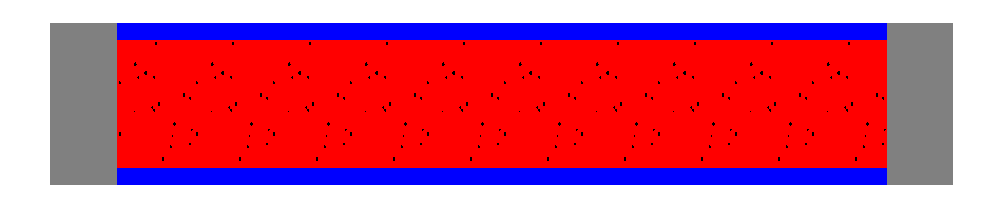
\includegraphics[width=\linewidth]{slab-obj-2-pfppf-min-pf.png}
        \caption{\gls{AHTR} plank model with the most-minimized $PF_{total}$
        (corresponds to the orange dotted distribution in Figure 
        \ref{fig:slab-obj-2-pfppf-pareto-distr}).}
        \label{fig:slab-obj-2-pfppf-min-pf} 
    \end{subfigure}
    \begin{subfigure}{\textwidth}
        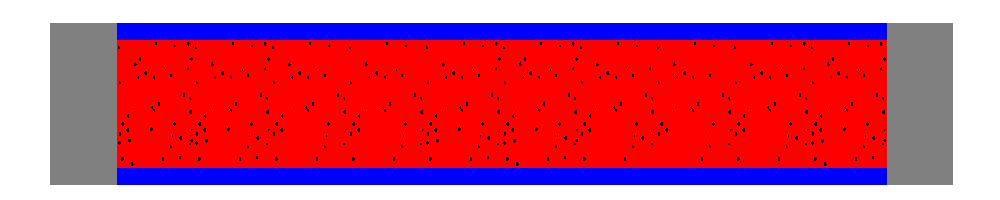
\includegraphics[width=\linewidth]{slab-obj-2-pfppf-min-ppf.png}
        \caption{\gls{AHTR} plank model with the most-minimized $PPF_{fuel}$
        (corresponds to the blue solid distribution in Figure 
        \ref{fig:slab-obj-2-pfppf-pareto-distr}).}
        \label{fig:slab-obj-2-pfppf-min-ppf} 
    \end{subfigure}
    \caption{(contd.) Simulation p-2b -- ROLLO two-objective optimization to minimize 
    total packing fraction ($PF_{total}$) and fuel-normalized power peaking factor 
    ($PPF_{fuel}$) in the plank. 
    Input parameters varied: TRISO packing fraction distribution ($\rho_{TRISO}(\vec{r})$).}
\end{figure}

All reactor models on Figure \ref{fig:slab-obj-2-pfppf}'s Pareto front have a relatively 
flat TRISO packing fraction distribution, varying between 0.02 and 0.04. 
In Figure \ref{fig:slab-obj-2-pfppf-pareto-distr}, the plank model with the 
most-minimized $PF_{total}$ and highest $PPF_{fuel}$
(the orange distribution) has a constant TRISO distribution of $PF_{total}=0.02$ 
across the plank (also illustrated in Figure \ref{fig:slab-obj-2-pfppf-min-pf}). 
In Figure \ref{fig:slab-obj-2-pfppf-pareto-distr}, the plank model with the 
most-minimized $PPF_{fuel}$ and highest $PF_{total}$
(the blue distribution) has a TRISO distribution that peaks in the center of the plank
and on both sides (also illustrated in Figure \ref{fig:slab-obj-2-pfppf-min-ppf}). 
Sections \ref{sec:plank-discussion-ppf-results} and \ref{sec:plank-discussion-multi}  
discuss and explain simulation p-2b's results.

\subsection{p-2c: Minimize $T_{max}$ and $PPF_{fuel}$}
\label{sec:p-2c}
This section reports results from the two-objective optimization simulation p-2c; the 
objectives minimized are maximum plank temperature ($T_{max}$) and fuel-normalized 
power peaking factor ($PPF_{fuel}$).  
Table \ref{tab:simulationp2c} shows simulation p-2c's optimization problem parameters. 
\begin{table}[htbp!]
    \centering
    \onehalfspacing
    \caption{Simulation p-2c optimization problem parameters.}
	\label{tab:simulationp2c}
    \footnotesize
    \begin{tabular}{l|p{4cm}}
    \hline 
    \multicolumn{2}{c}{\textbf{Two Objectives: Simulation p-2c}} \\
    \hline 
    \textbf{Objectives} & Minimize $T_{max}$ \\
    & Minimize $PPF_{fuel}$ \\
    \hline 
    \textbf{Input parameter variations} 
    & $\rho_{TRISO}(\vec{r})$: $0<a<2$ \\
    & $\rho_{TRISO}(\vec{r})$: $0<b<\frac{\pi}{2}$ \\
    & $\rho_{TRISO}(\vec{r})$: $0<c<2\pi$ \\
    \hline
    \textbf{Constraints} & $k_{eff} \geq 1.0$\\ 
    & $PF_{total}$ = 0.0979\\
    \hline 
    \textbf{Genetic algorithm parameters} & Population size: 120 \\
    & Generations: 3 \\
    \hline
    \end{tabular}
\end{table}

Table \ref{tab:p2c-hypervolume} shows each generation's hypervolume value, 
confirming that simulation p-2c converges by generation 3. 
\begin{table}[htbp!]
    \centering
    \onehalfspacing
    \caption{Simulation p-2c hypervolume values at each generation.}
	\label{tab:p2c-hypervolume}
    \footnotesize
    \begin{tabular}{ll}
    \hline 
    \multicolumn{2}{c}{\textbf{Two Objectives: Simulation p-2c}} \\
    \multicolumn{2}{c}{Reference point: (1300, 1.6)} \\
    \hline 
    \textbf{Generation} & \textbf{Hypervolume [-]} \\
    \hline
    1 & 92.041 \\
    2 & 92.087\\
    3 & 92.751 \\
    \hline
    \end{tabular}
\end{table}

Figure \ref{fig:slab-obj-2-tempppf-pareto} shows a plot of the final generation's 
reactor models' $T_{max}$ against $PPF_{fuel}$; crosses mark the reactor models that 
fall on the Pareto front.
Figure \ref{fig:slab-obj-2-tempppf-pareto-distr} shows the eight TRISO distributions in 
the final generation that fall on the Pareto front. 
Figures \ref{fig:slab-obj-2-tempppf-min-temp} and \ref{fig:slab-obj-2-tempppf-min-ppf} 
illustrate the \gls{AHTR} plank models with the most-minimized $T_{max}$ and 
$PPF_{fuel}$, respectively. 
\begin{figure}[htbp!]
    \centering
    \begin{subfigure}{\textwidth}
        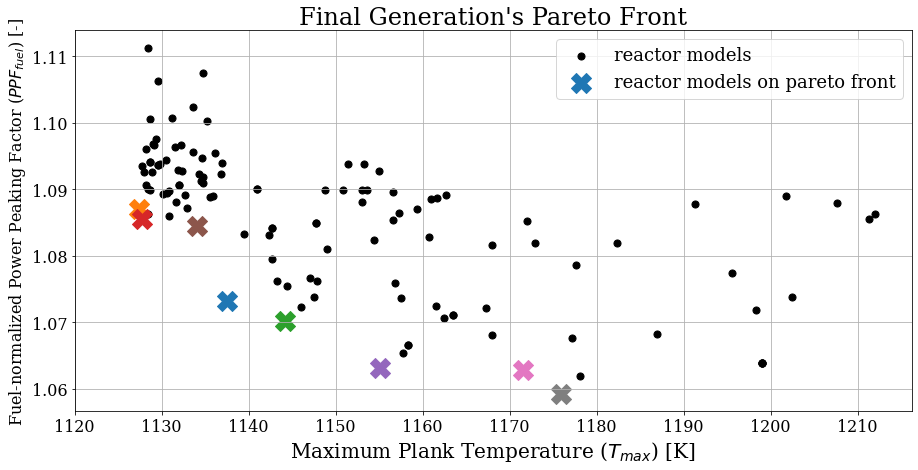
\includegraphics[width=\linewidth]{slab-obj-2-tempppf-pareto.png}
        \caption{Plot of final generation's reactor models' $T_{max}$ against 
        $PPF_{fuel}$. Crosses indicate the reactor models on the Pareto front.
        Cross colors correspond to TRISO distributions in the plot below.}
        \label{fig:slab-obj-2-tempppf-pareto} 
    \end{subfigure}
    \begin{subfigure}{\textwidth}
        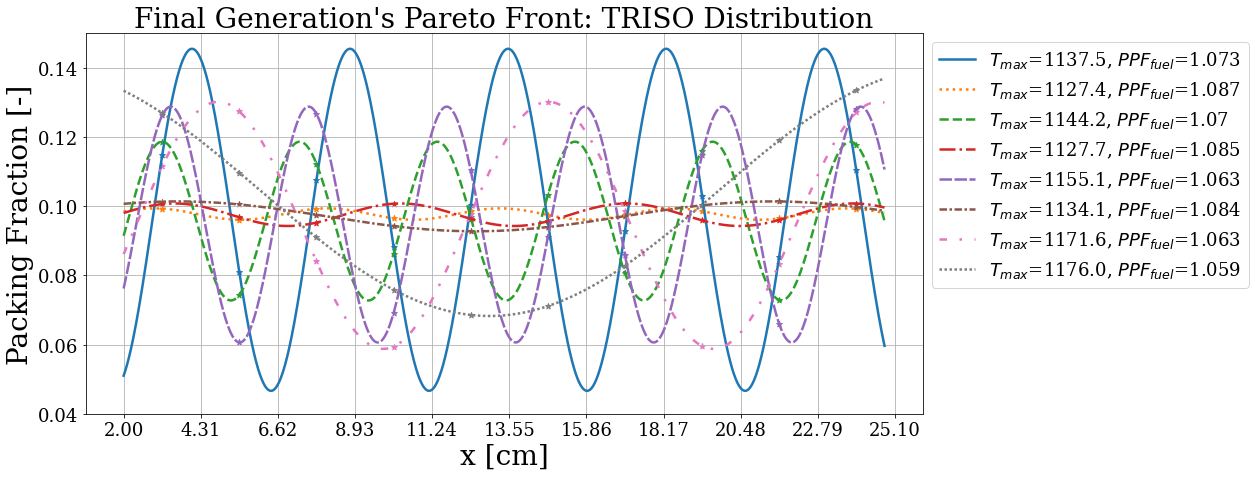
\includegraphics[width=\linewidth]{slab-obj-2-tempppf-pareto-distr.png}
        \caption{TRISO packing fraction distribution for the eight reactor models on the 
        Pareto front.}
        \label{fig:slab-obj-2-tempppf-pareto-distr} 
    \end{subfigure}
    \caption{Simulation p-2c -- ROLLO two-objective optimization to minimize the 
    maximum plank temperature ($T_{max}$) and fuel-normalized power peaking factor 
    ($PPF_{fuel}$) in the plank. 
    Input parameters varied: TRISO packing fraction distribution 
    ($\rho_{TRISO}(\vec{r})$). $PF_{total}$ = 0.0979.}
    \label{fig:slab-obj-2-tempppf}
\end{figure}
\begin{figure}[htbp!]
    \ContinuedFloat
    \begin{subfigure}{\textwidth}
        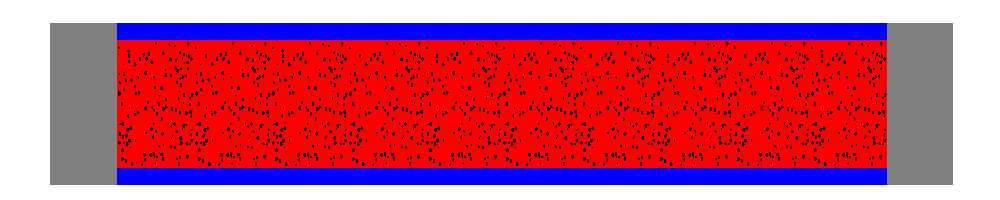
\includegraphics[width=\linewidth]{slab-obj-2-tempppf-min-temp.png}
        \caption{\gls{AHTR} plank model with the most-minimized $T_{max}$
        (corresponds to the orange dashed distribution in Figure 
        \ref{fig:slab-obj-2-tempppf-pareto-distr}).}
        \label{fig:slab-obj-2-tempppf-min-temp} 
    \end{subfigure}
    \begin{subfigure}{\textwidth}
        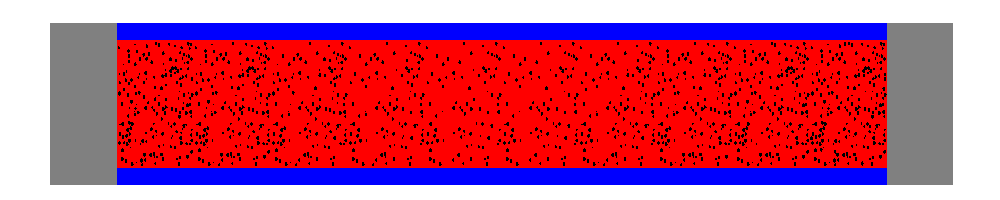
\includegraphics[width=\linewidth]{slab-obj-2-tempppf-min-ppf.png}
        \caption{\gls{AHTR} plank model with the most-minimized $PPF_{fuel}$
        (corresponds to the grey densely dotted distribution in Figure 
        \ref{fig:slab-obj-2-tempppf-pareto-distr}).}
        \label{fig:slab-obj-2-tempppf-min-ppf} 
    \end{subfigure}
    \caption{(contd.) Simulation p-2c -- ROLLO two-objective optimization to minimize 
    the maximum plank temperature ($T_{max}$) and fuel-normalized power peaking factor 
    ($PPF_{fuel}$) in the plank. 
    Input parameters varied: TRISO packing fraction distribution 
    ($\rho_{TRISO}(\vec{r})$). $PF_{total}$ = 0.0979.}
\end{figure}

In Figure \ref{fig:slab-obj-2-tempppf-pareto}, \gls{ROLLO} finds eight widely spread 
reactor model solutions on simulation p-2c's Pareto front. 
These \gls{TRISO} distributions on the Pareto front that minimize both $T_{max}$ 
and $PPF_{fuel}$ vary between the two extreme cases: 
most-minimized $T_{max}$ and most-minimized $PPF_{fuel}$.
In Figure \ref{fig:slab-obj-2-tempppf-pareto-distr}, the plank model with 
the most-minimized $T_{max}$ and highest $PPF_{fuel}$ (the orange dashed distribution) 
has an almost constant TRISO distribution of $PF_{total}=0.0979$ across the plank, 
with a slight oscillating pattern (also illustrated in Figure 
\ref{fig:slab-obj-2-tempppf-min-temp}).
In Figure \ref{fig:slab-obj-2-tempppf-pareto-distr}, the plank model with the
most-minimized $PPF_{fuel}$ and highest $T_{max}$ (the grey densely dotted 
distribution) has a TRISO distribution that peaks near the plank's sides and has 
a minimum point at the plank's center (also illustrated in Figure 
\ref{fig:slab-obj-2-tempppf-min-ppf}). 
Sections \ref{sec:plank-discussion-ppf-results} and \ref{sec:plank-discussion-multi} 
discuss and explain simulation p-2c's results.

\section{AHTR Plank: Three-Objective Optimization Results}
\label{sec:plank-three-obj}
This section reports the \gls{AHTR} plank's \gls{ROLLO} three-objective 
optimization results. 
Table \ref{tab:slab-obj-breakdown} summarized the three-objective simulations in this 
section: p-3a, and p-3b. 

\subsection{p-3a: Variation of $PF_{total}$ and $\rho_{TRISO}(\vec{r})$}
\label{sec:p-3a}
This section reports results from the three-objective optimization simulation p-3a, 
with all objectives minimized: total fuel packing fraction ($PF_{total}$), 
maximum plank temperature ($T_{max}$), and fuel-normalized power peaking factor 
($PPF_{fuel}$).  
The input parameters varied are total fuel packing fraction ($PF_{total}$) and 
TRISO packing fraction distribution ($\rho_{TRISO}(\vec{r})$). 
Table \ref{tab:simulationp3a} shows simulation p-3a's optimization problem parameters. 
\begin{table}[htbp!]
    \centering
    \onehalfspacing
    \caption{Simulation p-3a optimization problem parameters.}
	\label{tab:simulationp3a}
    \footnotesize
    \begin{tabular}{l|p{4cm}}
    \hline 
    \multicolumn{2}{c}{\textbf{Three Objectives: Simulation p-3a}} \\
    \hline 
    \textbf{Objectives} & Minimize $PF_{total}$ \\
    & Minimize $T_{max}$ \\
    & Minimize $PPF_{fuel}$ \\
    \hline 
    \textbf{Input parameter variations} & $0.02 \leq PF_{total} \leq 0.04$ \\
    & $\rho_{TRISO}(\vec{r})$: $0<a<2$ \\
    & $\rho_{TRISO}(\vec{r})$: $0<b<\frac{\pi}{2}$ \\
    & $\rho_{TRISO}(\vec{r})$: $0<c<2\pi$ \\
    \hline
    \textbf{Constraints} & $k_{eff} \geq 1.35$\\ 
    \hline 
    \textbf{Genetic algorithm parameters} & Population size: 128 \\
    & Generations: 5 \\
    \hline
    \end{tabular}
\end{table}

Table \ref{tab:p3a-hypervolume} shows each generation's hypervolume value, 
confirming that simulation p-3a converges by generation 5. 
\begin{table}[htbp!]
    \centering
    \onehalfspacing
    \caption{Simulation p-3a hypervolume values at each generation.}
	\label{tab:p3a-hypervolume}
    \footnotesize
    \begin{tabular}{ll}
    \hline 
    \multicolumn{2}{c}{\textbf{Three Objectives: Simulation p-3a}} \\
    \multicolumn{2}{c}{Reference point: (0.06, 1260 ,1.5)} \\
    \hline 
    \textbf{Generation} & \textbf{Hypervolume [-]} \\
    \hline
    1 & 2.392 \\
    2 & 2.392 \\
    3 & 2.393 \\
    4 & 2.442 \\
    5 & 2.446 \\
    \hline
    \end{tabular}
\end{table}

Figure \ref{fig:slab-obj-3-3d} shows a plot of the final generation's reactor models' 
$PF_{total}$ against $T_{max}$ against $PPF_{fuel}$; crosses 
mark the reactor models that fall on the Pareto front.
Figure \ref{fig:slab-obj-3-distr} shows the 14 TRISO packing fraction distributions in 
the final generation that fall on the Pareto front. 
\begin{figure}[htbp!]
    \begin{subfigure}{\textwidth}
        \centering
        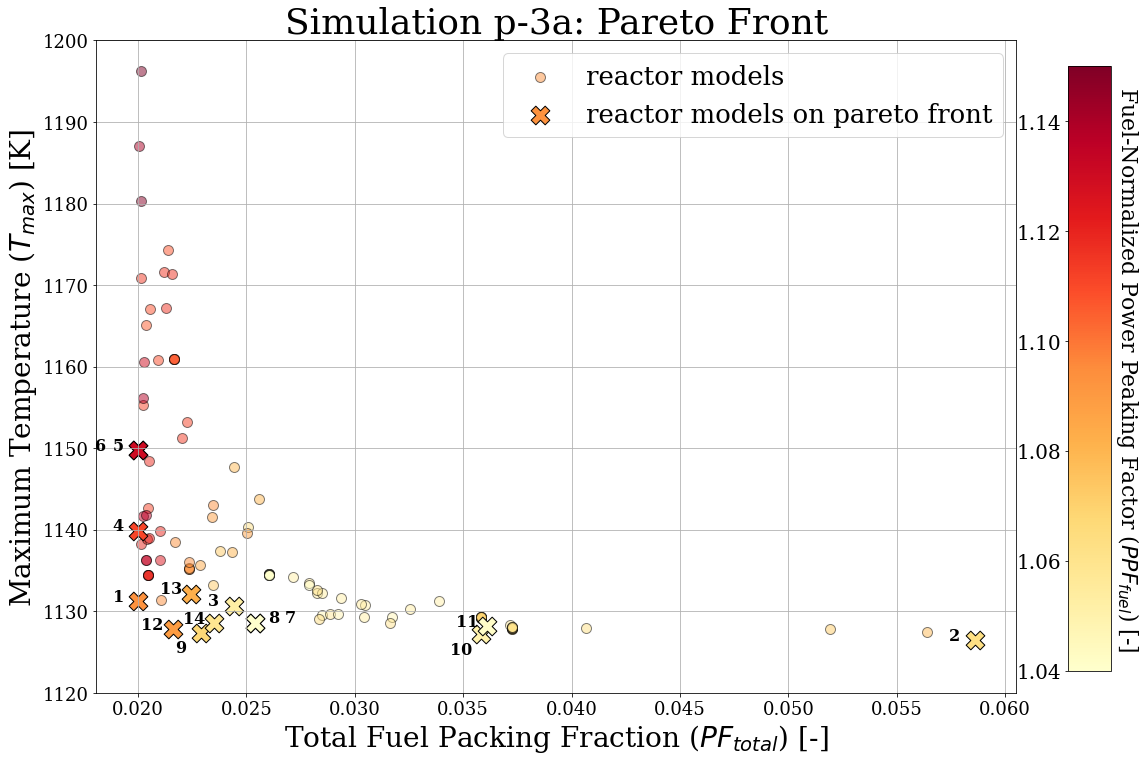
\includegraphics[width=\linewidth]{slab-obj-3-3d.png}
        \caption{Plot of final generation's reactor models' $PF_{total}$ against 
        $T_{max}$ against $PPF_{fuel}$ as a color dimension. 
        Crosses indicate the reactor models on the Pareto front. 
        Cross numbering correspond to TRISO distributions in Figure 
        \ref{fig:slab-obj-3-distr}.}
        \label{fig:slab-obj-3-3d} 
    \end{subfigure}
    \begin{subfigure}{\textwidth}
        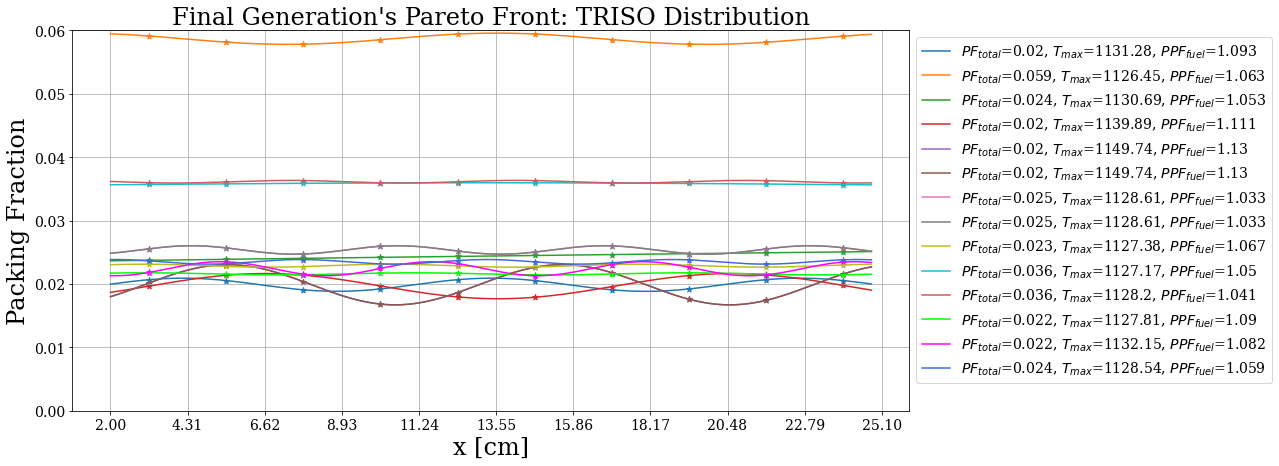
\includegraphics[width=\linewidth]{slab-obj-3-distr.png}
        \caption{TRISO packing fraction distribution for the 14 reactor models on the 
        Pareto front. Numbered reactor models correspond to numbered crosses in Figure 
        \ref{fig:slab-obj-3-3d}.}
        \label{fig:slab-obj-3-distr} 
    \end{subfigure}
    \caption{Simulation p-3a -- ROLLO three-objective optimization to minimize the total 
    fuel packing fraction ($PF_{total}$), maximum plank temperature ($T_{max}$) and 
    fuel-normalized power peaking factor ($PPF_{fuel}$) in the plank. 
    Input parameters varied: $PF_{total}$, TRISO packing fraction distribution
    ($\rho_{TRISO}(\vec{r})$).}
    \label{fig:slab-obj-3}
\end{figure}

Figure \ref{fig:slab-obj-3-3d} demonstrates that \gls{ROLLO} found 14 widely spread 
solutions in the final generation's Pareto front.  
Figure \ref{fig:slab-obj-3-distr-most-minimized} shows the three distributions from 
Figure \ref{fig:slab-obj-3-distr} that most-minimized each objective, respectively. 
Figures \ref{fig:slab-obj-3-min-pf}, \ref{fig:slab-obj-3-min-temp}, and 
\ref{fig:slab-obj-3-min-ppf} show the \gls{AHTR} plank's TRISO distribution and 
coolant channel shape for most-minimized cases. 
\begin{figure}[htbp!]
    \centering
    \begin{subfigure}{0.85\textwidth}
        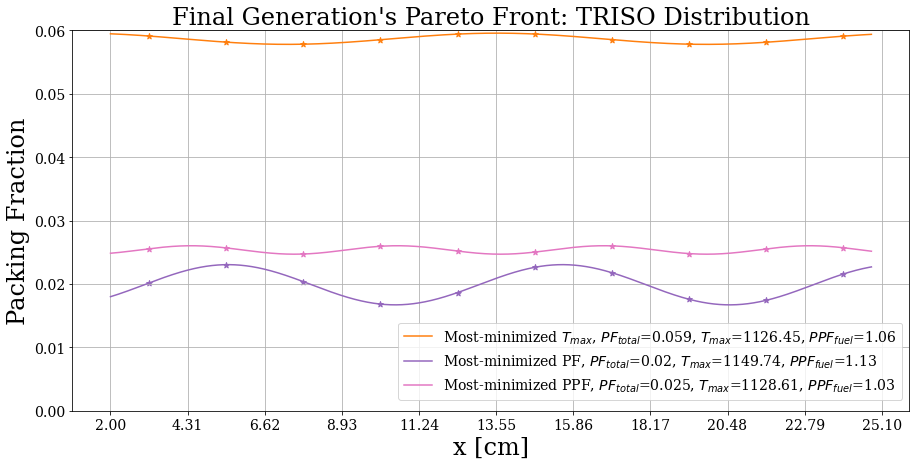
\includegraphics[width=\linewidth]{slab-obj-3-distr-most-minimized.png}
        \caption{TRISO distributions for the reactor models on the Pareto front
        that most-minimized each objective.}
        \label{fig:slab-obj-3-distr-most-minimized}
    \end{subfigure}
    \begin{subfigure}{0.8\textwidth}
        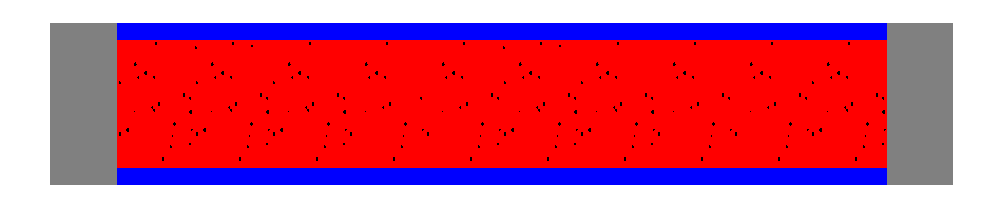
\includegraphics[width=\linewidth]{slab-obj-3-min-pf.png}
        \caption{\gls{AHTR} plank model with the most-minimized $PF_{total}$ 
        (corresponds to reactor model 5, the purple dashed distribution in 
        Figure \ref{fig:slab-obj-3-distr-most-minimized}.)}
        \label{fig:slab-obj-3-min-pf} 
    \end{subfigure}
    \begin{subfigure}{0.8\textwidth}
        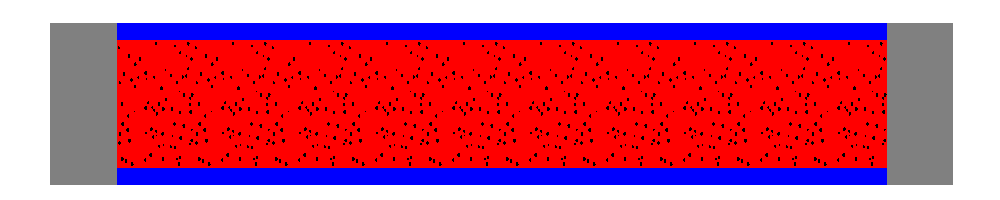
\includegraphics[width=\linewidth]{slab-obj-3-min-temp.png}
        \caption{\gls{AHTR} plank model with the most-minimized $T_{max}$
        (corresponds to reactor model 2, the orange dotted distribution in
        Figure \ref{fig:slab-obj-3-distr-most-minimized}.)}
        \label{fig:slab-obj-3-min-temp} 
    \end{subfigure}
    \begin{subfigure}{0.8\textwidth}
        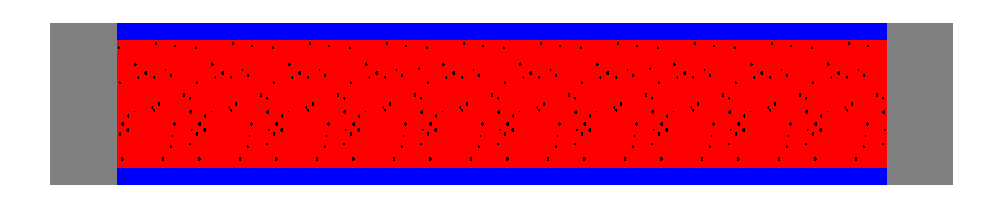
\includegraphics[width=\linewidth]{slab-obj-3-min-ppf.png}
        \caption{\gls{AHTR} plank model with the most-minimized $PPF_{fuel}$
        (corresponds to reactor model 7, the pink solid distribution in
        Figure \ref{fig:slab-obj-3-distr-most-minimized}.)}
        \label{fig:slab-obj-3-min-ppf} 
    \end{subfigure}
    \caption{AHTR plank models and TRISO distribution for the 3 reactor models on 
    simulation p-3a's Pareto front that most-minimized each objective.
    Simulation p-3a -- ROLLO three-objective optimization to minimize the total fuel 
    packing fraction ($PF_{total}$), maximum plank temperature ($T_{max}$) and 
    normalized power peaking factor ($PPF_{fuel}$) in the plank. 
    Input parameters varied: $PF_{total}$, TRISO packing fraction distribution
    ($\rho_{TRISO}(\vec{r})$)}
    \label{fig:slab-obj-3-most-minimized}
\end{figure}

In Figure \ref{fig:slab-obj-3-distr-most-minimized}, reactor model 5 with the
most-minimized $PF_{total}$ (the purple dashed distribution) has an oscillating TRISO 
distribution with $\sim0.01$ variation and $PF_{total} = 0.02$ 
(also illustrated in Figure \ref{fig:slab-obj-3-min-pf}).
In Figure \ref{fig:slab-obj-3-distr-most-minimized}, reactor model 2 with the 
most-minimized $T_{max}$ (the orange dotted distribution) has an almost constant TRISO 
distribution of $PF_{total}=0.059$ (also illustrated in Figure 
\ref{fig:slab-obj-3-min-temp}). 
In Figure \ref{fig:slab-obj-3-distr-most-minimized}, reactor model 7 with the
most-minimized $PPF_{fuel}$ (the pink solid distribution) has a 
slightly oscillating TRISO distribution and $PF_{total} = 0.025$ 
(also illustrated in Figure \ref{fig:slab-obj-3-min-ppf}).
Section \ref{sec:plank-discussion-multi} discusses and explains simulation p-3a's results.

\subsection{p-3b: Variation of $PF_{total}$, $\rho_{TRISO}(\vec{r})$, and Coolant 
Channel Shape}
\label{sec:p-3b}
This section reports results from the three-objective optimization simulation p-3b, 
with all objectives minimized: total fuel packing fraction ($PF_{total}$), maximum plank 
temperature ($T_{max}$), and fuel-normalized power peaking factor ($PPF_{fuel}$).  
The input parameters varied are total fuel packing fraction ($PF_{total}$), 
TRISO packing fraction distribution ($\rho_{TRISO}(\vec{r})$), and coolant channel 
shape.  
Table \ref{tab:simulationp3b} shows simulation p-3b's optimization problem parameters. 
\begin{table}[htbp!]
    \centering
    \onehalfspacing
    \caption{Simulation p-3b optimization problem parameters.}
	\label{tab:simulationp3b}
    \footnotesize
    \begin{tabular}{l|p{6.5cm}}
    \hline 
    \multicolumn{2}{c}{\textbf{Three Objectives: Simulation p-3b}} \\
    \hline 
    \textbf{Objectives} & Minimize $PF_{total}$ \\
    & Minimize $T_{max}$ \\
    & Minimize $PPF_{fuel}$ \\
    \hline 
    \textbf{Input parameter variations} & $0.02 \leq PF_{total} \leq 0.04$ \\
    & $\rho_{TRISO}(\vec{r})$: $0<a<2$ \\
    & $\rho_{TRISO}(\vec{r})$: $0<b<\frac{\pi}{2}$ \\
    & $\rho_{TRISO}(\vec{r})$: $0<c<2\pi$ \\
    & Coolant channel shape: $0.05<r_{top}<0.35$ \\
    & Coolant channel shape: $0.05<r_{bot}<0.35$ \\
    \hline
    \textbf{Constraints} & $k_{eff} \geq 1.35$\\ 
    \hline 
    \textbf{Genetic algorithm parameters} & Population size: 128 \\
    & Generations: 8 \\
    \hline
    \end{tabular}
\end{table}

Table \ref{tab:p3b-hypervolume} shows each generation's hypervolume value, 
confirming that simulation p-3b converges by generation 8. 
\begin{table}[htbp!]
    \centering
    \onehalfspacing
    \caption{Simulation p-3b hypervolume values at each generation.}
	\label{tab:p3b-hypervolume}
    \footnotesize
    \begin{tabular}{ll}
    \hline 
    \multicolumn{2}{c}{\textbf{Three Objectives: Simulation p-3b}} \\
    \multicolumn{2}{c}{Reference point: (0.06, 1260 ,1.5)} \\
    \hline 
    \textbf{Generation} & \textbf{Hypervolume [-]} \\
    \hline
    1 & 1.985 \\
    2 & 2.119 \\
    3 & 2.158 \\
    4 & 2.251\\
    5 & 2.262 \\
    6 & 2.280 \\
    7 & 2.310 \\
    8 & 2.313 \\
    \hline
    \end{tabular}
\end{table}

Figure \ref{fig:slab-obj-3-3d-all} shows a plot of the final generation's reactor 
models' $PF_{total}$ against $T_{max}$ against $PPF_{fuel}$; 
crosses mark the reactor models that fall on the Pareto front.
Figure \ref{fig:slab-obj-3-distr-all} shows the 21 TRISO distributions and their
total radius ($r_{top}, r_{bot}$) in the final generation that fall on the Pareto 
front. 
\begin{figure}[htbp!]
    \begin{subfigure}{\textwidth}
        \centering
        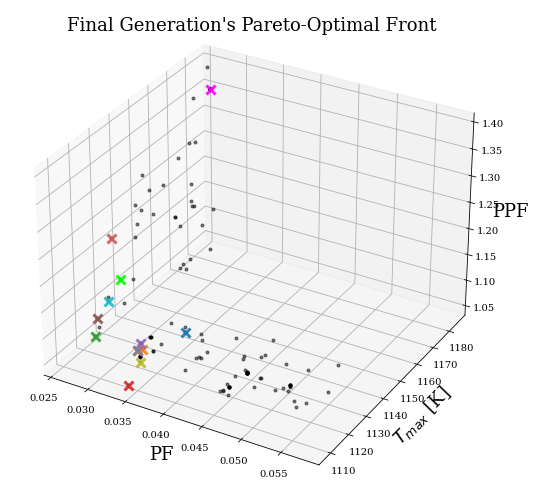
\includegraphics[width=\linewidth]{slab-obj-3-3d-all.png}
        \caption{Plot of final generation's reactor models' $PF_{total}$ against 
        $T_{max}$ against $PPF_{fuel}$ as a color dimension. 
        Crosses indicate the reactor models on the 
        Pareto front. Cross numbering correspond to TRISO distributions in Figure 
        \ref{fig:slab-obj-3-distr-all}.}
        \label{fig:slab-obj-3-3d-all} 
    \end{subfigure}
    \begin{subfigure}{\textwidth}
        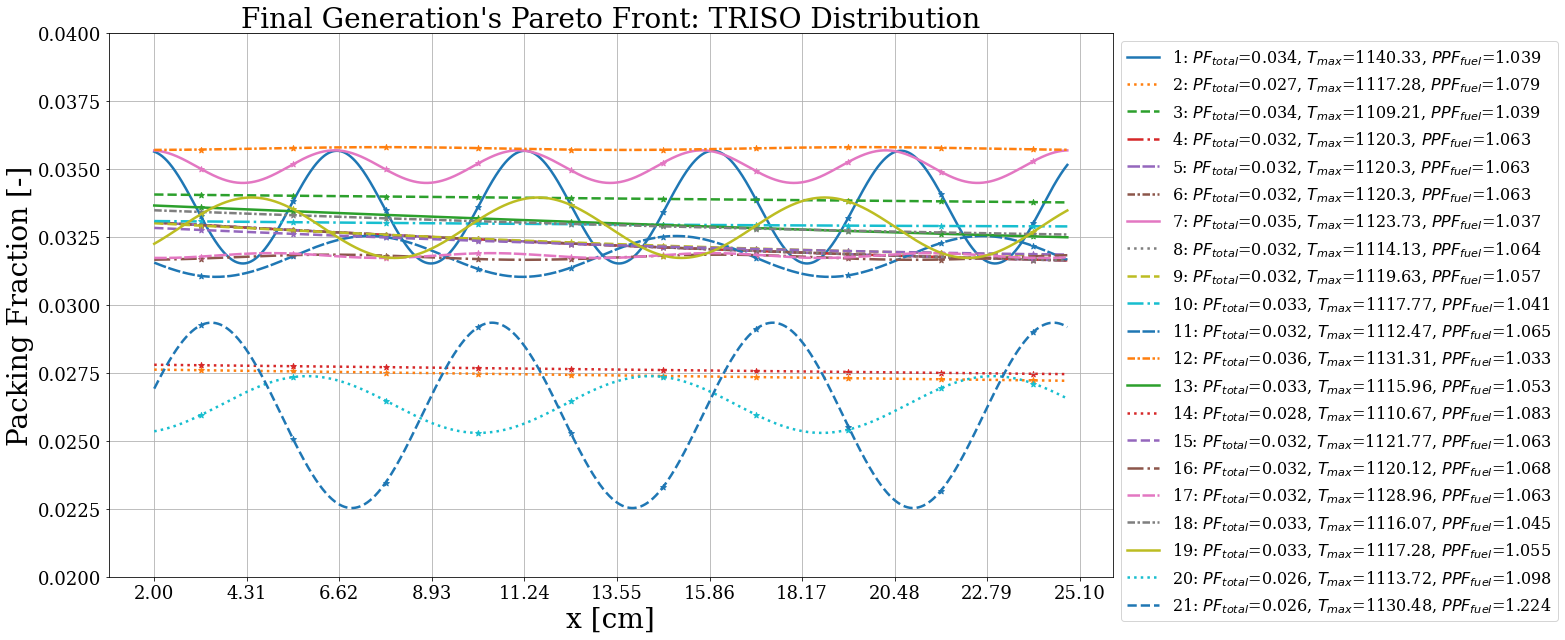
\includegraphics[width=\linewidth]{slab-obj-3-distr-all.png}
        \caption{TRISO distribution for the 21 reactor models on the Pareto front.}
        \label{fig:slab-obj-3-distr-all} 
    \end{subfigure}
    \caption{Simulation p-3b -- ROLLO three-objective optimization to minimize the total 
    fuel packing fraction ($PF_{total}$), maximum plank temperature ($T_{max}$), and 
    fuel-normalized power peaking factor ($PPF_{fuel}$) in the plank. 
    Input parameters varied: total fuel packing fraction $PF_{total}$, 
    TRISO packing fraction distribution ($\rho_{TRISO}(\vec{r})$), 
    coolant channel shape $(r_{top}, r_{bot})$.}
    \label{fig:slab-obj-3-all}
\end{figure}

Figure \ref{fig:slab-obj-3-3d-all} demonstrates that \gls{ROLLO} found 21 widely spread 
solutions in the final generation's Pareto front. 
Figure \ref{fig:slab-obj-3-distr-most-minimized-distr-all} shows the three distributions 
from Figure \ref{fig:slab-obj-3-distr-all} that most-minimized each objective, 
respectively.
Figures \ref{fig:slab-obj-3-all-min-pf}, \ref{fig:slab-obj-3-all-min-temp}, and 
\ref{fig:slab-obj-3-all-min-ppf} show the \gls{AHTR} plank's TRISO distribution and 
coolant channel shape for most-minimized cases. 
\begin{figure}[htbp!]
    \begin{subfigure}{\textwidth}
        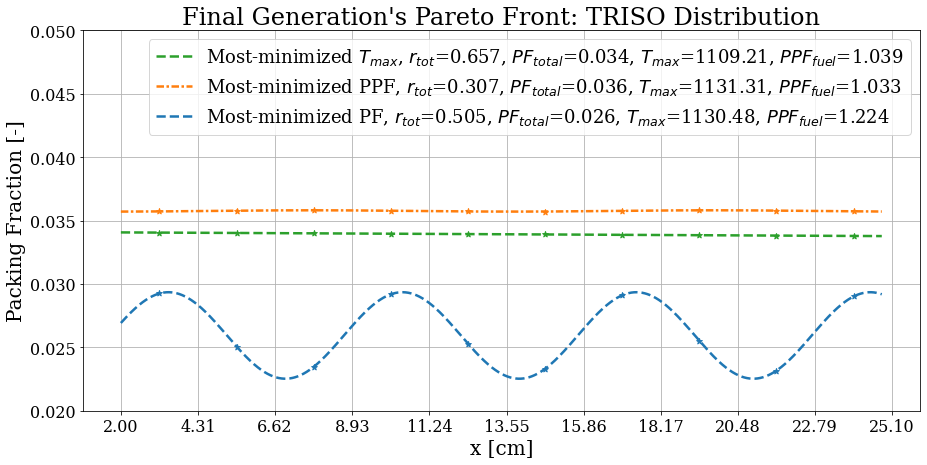
\includegraphics[width=\linewidth]{slab-obj-3-distr-most-minimized-all.png}
        \caption{TRISO distributions for the reactor models on the Pareto 
        front that most minimized each objective.}
        \label{fig:slab-obj-3-distr-most-minimized-distr-all}
    \end{subfigure}
    \begin{subfigure}{\textwidth}
        
\includegraphics[width=\linewidth]{slab-obj-3-all-min-pf.png}
        \caption{\gls{AHTR} plank model with the most-minimized $PF_{total}$ 
        (corresponds to reactor model 21, the blue dashed distribution in 
        Figure \ref{fig:slab-obj-3-distr-most-minimized-distr-all}.)}
        \label{fig:slab-obj-3-all-min-pf}
    \end{subfigure}
    \begin{subfigure}{\textwidth}
        
\includegraphics[width=\linewidth]{slab-obj-3-all-min-temp.png}
        \caption{\gls{AHTR} plank model with the most-minimized $T_{max}$
        (corresponds to reactor model 3, the green straight dashed distribution 
        in Figure \ref{fig:slab-obj-3-distr-most-minimized-distr-all}.)}
        \label{fig:slab-obj-3-all-min-temp}
    \end{subfigure}
    \begin{subfigure}{\textwidth}
        
\includegraphics[width=\linewidth]{slab-obj-3-all-min-ppf.png}
        \caption{\gls{AHTR} plank model with the most-minimized $PPF_{fuel}$
        (corresponds to reactor model 12, the orange dashdot distribution 
        in Figure \ref{fig:slab-obj-3-distr-most-minimized-distr-all}.).}
        \label{fig:slab-obj-3-all-min-ppf}
    \end{subfigure}
    \caption{AHTR models and TRISO distribution for the 3 reactor models on simulation 
    p-3b -- ROLLO three-objective optimization to minimize the total 
    fuel packing fraction ($PF_{total}$), maximum plank temperature ($T_{max}$), and 
    fuel-normalized power peaking factor ($PPF_{fuel}$) in the plank. 
    Input parameters varied: total fuel packing fraction $PF_{total}$, 
    TRISO packing fraction distribution ($\rho_{TRISO}(\vec{r})$), 
    coolant channel shape $(r_{top}, r_{bot})$.}
    \label{fig:slab-obj-3-distr-most-minimized-all}
\end{figure}

In Figure \ref{fig:slab-obj-3-distr-most-minimized-distr-all}, the \gls{AHTR} plank model 
with the most-minimized $PF_{total}$ (the blue dashed distribution) has an 
oscillating TRISO distribution with approximately $\sim0.01cm$ of variation, 
$PF_{total} = 0.026$, and $r_{tot}=0.505cm$ (illustrated in Figure 
\ref{fig:slab-obj-3-all-min-pf}).
In Figure \ref{fig:slab-obj-3-distr-most-minimized-distr-all}, the \gls{AHTR} plank 
model with the most-minimized $T_{max}$ (the green dashed distribution) has a constant 
TRISO distribution of $PF_{total}=0.034$ and $r_{tot}=0.657cm$
(illustrated in Figure \ref{fig:slab-obj-3-all-min-temp}).
In Figure \ref{fig:slab-obj-3-distr-most-minimized-distr-all}, the \gls{AHTR} plank 
model with the most-minimized $PPF_{fuel}$ (the orange dashdot distribution) has a 
constant TRISO distribution of $PF_{total} = 0.036$ and $r_{tot}=0.307cm$
(illustrated in Figure \ref{fig:slab-obj-3-all-min-ppf}).
Section \ref{sec:plank-discussion-multi} discusses and explains simulation p-3b's 
results.

\section{AHTR Plank: Computational Cost Summary}
\label{sec:plank-compute-cost}
The optimization simulations for this work were run on the BlueWaters supercomputer 
\cite{ncsa_about_2017} and the Theta supercomputer at the Argonne Leadership Computing 
Facility under the Director's Discretionary Allocation Program 
\cite{noauthor_argonne_2022}. 
Each BlueWaters XE compute node has 32 Interlagos processor cores with a nominal 
clock speed of 3.2GHz \cite{ncsa_about_2017}, and each Theta compute node is a single 
Xeon Phi chip with 64 cores with a nominal clock speed of 1.5GHz 
\cite{noauthor_argonne_2022}.  

Each optimization simulation takes a different amount of node-hours to run due to 
differences in simulation software, tallies, and intermediate steps required. 
Table \ref{tab:plank-compute-cost} reports the computational cost for each optimization 
simulation. 
One may refer to Table \ref{tab:slab-obj-breakdown} for each simulation's parameters.
\begin{table}[htbp!]
    \centering
    \onehalfspacing
    \caption{Computational cost of \gls{ROLLO} simulations for optimizing \gls{AHTR}
    plank. BW: BlueWaters Supercomputer, Theta: Theta Supercomputer.}
	\label{tab:plank-compute-cost}
    \footnotesize
    \begin{tabular}{p{1.4cm}|p{1cm}lp{3.5cm}lp{3.5cm}}
    \hline 
    \textbf{Num of Objs} & \textbf{Sim} & \textbf{Machine} & 
    \textbf{Compute Cost Per Gen [node-hours]} &\textbf{Generations [\#]} & 
    \textbf{Total Compute Cost [node-hours]} \\
    \hline
    \multirow{6}{2cm}{1} 
    & p-1a & BW & 23.9 & 10 & 238.7 \\
    & p-1b & BW & 96.0 & 10 & 959.7 \\
    & p-1c & BW & 65.9 & 10 & 658.6 \\
    & p-1d & Theta & 49.6 & 3 & 148.7 \\
    & p-1e & Theta & 71.4 & 4 & 285.6 \\
    & p-1f & Theta & 46.4 & 5 & 231.8 \\
    \hline
    \multirow{3}{2cm}{2}
    & p-2a & Theta & 132.2 & 2 & 264.5 \\
    & p-2b & Theta & 66.3 & 3 & 198.9 \\
    & p-2c & Theta & 167.1 & 3 & 501.2 \\
    \hline
    \multirow{2}{2cm}{3}
    & p-3a & Theta & 92.9 & 5 & 464.5 \\
    & p-3b & Theta & 178.2 & 8 & 1425.8 \\
    \hline
    \end{tabular}
\end{table}

\pagebreak
\section{Summary}
\glsresetall
This chapter described the \gls{AHTR} plank's \gls{ROLLO} optimization results. 
I varied the following \gls{AHTR} plank input parameters: \gls{TRISO} packing fraction 
distribution ($\rho_{TRISO}(\vec{r})$), total fuel packing fraction ($PF_{total}$), and 
coolant channel shape; in an effort to minimize the following objectives: total 
fuel packing fraction ($PF_{total}$), maximum plank temperature ($T_{max}$), and 
fuel-normalized power peaking factor ($PPF_{fuel}$). 

In Section \ref{sec:plank-one-obj}'s six single-objective optimization simulations
(p-1a, p-1b, p-1c, p-1d, p-1e, p-1f) and Sections \ref{sec:plank-discussion-pf}, 
\ref{sec:plank-discussion-temp}, and \ref{sec:plank-discussion-ppf} discussions,    
I characterized each objective's driving factors and relationship with each input 
parameter. 
I determined that the minimize $T_{max}$ objective is driven by minimizing plank's maximum 
temperature and, flattens TRISO distribution and maximizes coolant channel shape's 
$r_{tot}$ to achieve the objective. 
The minimize $PF_{total}$ objective is driven by maximizing the plank's total fission 
reaction rate and influences the TRISO disribution to achieve the objective. 
The minimize $PPF_{fuel}$ objective is driven by flattening the plank's thermal flux
distribution and influences $PF_{total}$ and TRISO disribution to achieve the objective. 
Both the minimize $PF_{total}$ and minimize $PPF_{fuel}$ objectives have no correlation 
with the coolant channel shape. 

In Sections \ref{sec:plank-two-obj} and \ref{sec:plank-three-obj}'s five multi-objective 
optimization simulations (p-2a, p-2b, p-2c, p-3a, and p-3b) and Section 
\ref{sec:plank-discussion-multi}'s discussions, I further analyzed how the objectives' 
combined effects resulted in the optimal reactor models found by each multi-objective 
optimization simulation. 
All the multi-objective optimization simulations successfully found a wide spread of 
reactor models on a Pareto front that meets each objective to varying degrees. 
In the multi-objective optimization simulations, the minimize $T_{max}$ objective 
continued to influence the flattening of the TRISO distribution and maximizing of the 
coolant channel shape ($r_{bot}$ and $r_{top}$) to achieve the objective. 
The results from simulation p-2b and investigations in Section 
\ref{sec:plank-discussion-ppf-results} suggested that the minimize $PF_{total}$ 
objective's driving factor maximize total fission reaction rate and 
minimize $PPF_{fuel}$ objective's driving factor flattening thermal flux distribution 
influence each other resulting in unexpected TRISO distributions at different 
$PF_{total}$ values. 
Simulation p-3b's multi-objective optimization shows the result of minimizing all 
three objectives (minimize $PF_{total}$, $T_{max}$, and $PPF_{fuel}$) while varying 
all the input parameters ($PF_{total}$, TRISO distribution, and coolant channel shape).
Figure \ref{fig:slab-obj-3-all} shows the 21 widely spread reactor models on simulation 
p-3b's Pareto front that meet the three objectives to varying degrees. 

This chapter demonstrated \gls{ROLLO}'s success in conducting multi-objective 
optimization, a global search of the large reactor design space, to find optimal reactor 
models on the Pareto front that satisfy all the objectives. 
Reactor designers can utilize \gls{ROLLO} for multi-objective optimization problems with 
any number of objectives and arbitrary input parameters, to narrow down the search space 
to find reactor models that meet their desired requirements. 
The results from \gls{ROLLO}'s multi-objective optimizations help reactor designers 
gain a clearer understanding of the reactor models' parameters that meet their defined 
objectives to varying degrees.
From there, reactor designers can determine the importance of each objective for 
their purposes, then conduct sensitivity analysis and use higher fidelity models to 
further study a smaller section of the optimal design space that they are 
interested in.

This chapter successfully determined and explained the driving factors behind 
each reactor optimization objective and their relationship with one another.  
Characterizations of each objective for a simple \gls{AHTR} plank model provides 
insights for the next chapter in which I conduct multi-objective optimization for 
the more complex \gls{AHTR} one-third assembly model. 
